\documentclass[twoside,a4paper,11pt]{memoir}

% fix incompatibility between memoir and graphicx packages, both using ifpdf
\makeatletter 
\let\saved@ifpdf\ifpdf 
\let\ifpdf\@undefined 
\usepackage{ifpdf} 
\@ifundefined{ifpdf}{% 
  \let\ifpdf\saved@ifpdf 
}{% 
  \ifx\ifpdf\saved@ifpdf 
  \else 
    \latex@error{Different meaning of \@backslash ifpdf}\@ehc 
  \fi   
} 
\makeatother

\usepackage{a4}
\usepackage{times}
\usepackage{pslatex}
\usepackage{url}
\usepackage{mscthesis}
\usepackage{lscape}
\usepackage{longtable}
\usepackage{paralist}
\usepackage{mdwlist}
\usepackage{hyperref}
\usepackage{color}
\definecolor{tud}{RGB}{0,166,214}

\hypersetup{
	pdftitle={Investigating the usefulness of stack traces in bug triaging},    % title
    pdfauthor={M.M. Krikke},     % author
	colorlinks=true,       % false: boxed links; true: colored links
    linkcolor=black,          % color of internal links
    citecolor=black,        % color of links to bibliography
    filecolor=black,      % color of file links
    urlcolor=black           % color of external links
}

% %% The package 'algorithm' is useful, but incompatible with memoir.
% %% Cor-Paul Bezemer / http://homes.esat.kuleuven.be/~dvherten/esatthesis.html
% %% suggest the following fix:
\let\newfloat\undefined \usepackage{algorithmic} 
\usepackage{algorithm}
\usepackage{graphicx}
\usepackage{color}
\usepackage{wrapfig}

\let\subcaption\relax
\let\subfloat\relax
\usepackage{caption}
\usepackage{subcaption}

\usepackage{booktabs}

% set font to Latin Modern
\usepackage{lmodern}
\usepackage[T1]{fontenc}

%---------------------------------------------------------------------%
%                     Options                                         %    
%---------------------------------------------------------------------%

\title{Investigating the usefulness of stack traces in bug triaging}
\subtitle{Master's Thesis}

\author{Marco Krikke}
\authoremail{\url{marcokrikke@student.tudelft.nl}}
\birthplace{Ede, The Netherlands}
\studentid{1156004}

% Optional (postscript) cover picture. Put this in comments when not needed.
%\coverpicture{\includegraphics[width=13cm]{img/maze.ps}}

% A copyright notice and maybe something about the cover picture
% Put in comments to get the default copyright notice
\colophon{\begin{wrapfigure}[2]{l}{1in}
	\vspace{-15pt}
	
\includegraphics[width=1in]{img/by-sa.png}
\end{wrapfigure}\noindent
This thesis is licensed under a \href{http://creativecommons.org/licenses/by-sa/3.0/}{Creative Commons Attribution-ShareAlike 3.0 Unported License}.
  %Cover picture: A ``random'' maze generated in postscript.
}

% thesis committee:
\chair{prof. dr. A. van Deursen, Faculty EEMCS, TU Delft}
\supervisor{dr. ir. M. Pinzger, Faculty EEMCS, TU Delft}
\committeemember{dr. S.O. Dulman, Faculty EEMCS, TU Delft}

\setcounter{tocdepth}{1}
\setsecnumdepth{subsection}
\maxsecnumdepth{subsection}

\begin{document}
\frontmatter
\thispagestyle{empty}
\maketitle                                      % for the cover page
\makeformaltitlepages{%!TEX root = thesis.tex

In software engineering, resources such as time, money and developers, are limited. Often when bugs are found in the software developed, bug triaging is used to prioritise bug reports and allocate resources to it. When the number of bugs is considerable, this will require a vast amount of time and effort. The goal of this research is to investigate the usefulness of stack traces in bug reports for the assessment of bug report properties, using existing metrics of bug reports and files, being severity, priority and time-to-fix.

In order to investigate the usefulness of stack traces, a research framework and methodology are developed. Overall, we can conclude that stack traces can be used to link software artifacts. Also, stack traces can be a valuable input for prediction models, for example using metrics of related bugs and source files. 



}         % for formal title pages with all info

%!TEX root = thesis.tex
\chapter{\label{cha:Preface}Preface}

This report is the result of my Master's thesis project performed at the Software Engineering Research Group (SERG) at Delft University of Technology. With this project I got the opportunity to research an aspect of software engineering I find most interesting: combining historical data to assist in every day software engineering processes, such as bug triaging.

Crafting this thesis took quite a while. Not only did I explore several other possibilities for a thesis project (that ended up not working out), also working on a thesis project \emph{and} running a successful company was really challenging. It was always a struggle to choose between business and thesis project, resulting quite often in a lack of focus.

But finally, after some hard work, focus, and determination, before you lies the result of my work. First of all, I would like to thank Ali Mesbah for supervising me during the first part of my literature research. After Ali left to pursue a career at the University of British Columbia, Martin Pinzger became my daily supervisor. Martin, first of all thank you for all your patience with me, it has been quite a ride. I really appreciated the interesting discussions we had and the guidance, support and feedback you offered me. Finally, thank you for keeping me focused towards my goal: finishing this thesis. 

To all others that helped me during my thesis project, in whatever manner, thank you for all your support and patience. 

\vskip1cm
\begin{flushright}
\theauthor\\
Delft, The Netherlands \\
August 17, 2012\\
\end{flushright}



\cleardoublepage\tableofcontents
\cleardoublepage\listoffigures
\cleardoublepage\mainmatter

\part{Introduction} % (fold)
\label{prt:introduction}
%!TEX root = thesis.tex

\chapter{\label{cha:intro}Introduction}
Medical treatment has been applied to humans for centuries, trying to help recover patients from their health problems. In some situations, the demand for medical resources is higher than the available resources. For example in battlefield situations or disasters, the number of patients needing treatment can be a lot higher than the available medical resources, such as personnel, transport and medicine. In these situations, not all patients can be treated immediately, and some may not be treated at all. 

The French baron Dominique--Jean Larrey is mostly attributed as the first person to devise a system to distribute available resources among the patient demand in the battlefield. Larrey was a Surgeon in Chief is the army of Napoleon Bonaparte, joining battle in Germany, Poland and Russia. Before the Napoleon Wars, injured soldiers were left in the battlefield, mainly taken care of by their fellow soldiers. Larrey however, evacuated wounded soldiers using `flying ambulances' and performed many treatments during the battle and even in the battlefield \cite{Baker2005}. 

In order to distribute his available medical resources among the wounded soldiers, Larrey used a system to sort patients for treatment. His memoirs state: 

\begin{quote}
\emph{Those who are dangerously wounded should receive the first attention, without regard to rank or distinction. They who are injured in a less degree may wait until their brethren in arms, who are badly mutilated, have been operated on and dressed, otherwise the latter would not survive many hours; rarely, until the succeeding day.} \cite{Mackersie}
\end{quote}

Nowadays, the term used to maximise benefit to the group of injured patients in the case where limited resources are available is called \emph{triaging}. The term originates from the French verb `trier', meaning `to sort'. 

\section{Research motivations}
In software engineering, resources such as time, money and developers, are also limited. Often when bugs are found in the software developed, \emph{bug triaging} is used to prioritise bug reports and allocate resources to it. Just as in a battlefield situations, not all `patients' might get `treatment'. For example, costs to fix a bug might outweigh the benefits, a bug is non-severe and will never be fixed, or a bug is a duplicate of an already fixed bug.

A bug triage can have several outcomes. Possibly, bugs are already reported and should be marked as duplicate. Otherwise, a 
\begin{inparaenum}[(1)]
\item severity and
\item priority should be assigned, a 
\item developer should be appointed, and a
\item target version should be chosen.
\end{inparaenum}
The severity of a bug (i.e., the impact of the bug) is not the same as the importance to fix a bug (i.e., the priority). For example, a crash of a program is quite severe, but when the crash only occurs under very specific conditions, the associated bug report might be assigned the lowest priority.

Bug triaging is a difficult process, where the \emph{triager} should have sufficient knowledge of the software product in order to make a good assessment of the bug report. The triager can use several sources to assess bug properties (e.g., severity, priority), such as software artifacts (source code, documentation), tools, existing knowledge and experience \cite{Panichella2012}. Bug triagers, even the most experienced ones, make mistakes, since they're always limited in their knowledge and experience. Mistakes, such as assigning a developer with little knowledge of the subsystem of the software where the bug occurs, can increase the fix time of a bug and can lead to low quality fixes \cite{Zimmermann2010,Bettenburg2007}.

In large (open source) software projects, the number of bug reports can be considerable. Possibly, a large community is reporting bugs, but it is also possible that bug reports are automatically collected. When each of these bugs should be analysed by a bug triager, this will require a vast amount of time and effort. Especially when taken into consideration the high overall knowledge of a system that is needed.

Automating certain tasks of a bug triager might be beneficial. For example, the detection of duplicate bugs saves a lot of time. Several studies already researched prediction models for priority and severity, mostly based on textual analysis \cite{Sun2011,Lamkanfi2010,Panichella2012}.

\section{Goal of this thesis} % (fold)
In order to assist the bug triager in the assessment of a bug, a large amount of data is already available, such as:

\begin{itemize*}
	\item documentation
	\item source code
	\item source code history in SCM systems (including patches, committers, et cetera)
	\item tests
	\item software models
	\item related bug reports
	\item stack traces in bug reports
\end{itemize*}

The goal of this research is to investigate the usefulness of \emph{stack traces} in bug reports for the assessment of bug report properties, such as severity, priority, time-to-fix and assigned developer. In order to achieve this, a research framework has been developed and an explorative study of a large data set has been performed. The most promising results are presented in this thesis.

\subsection{Possible application: assisting the bug triager} % (fold)
A possible application is the development of a prediction model to assist the bug triager. Stack traces can be used to relate bug reports to a bug report history that is built up over a vast amount of time. With this historical data, a prediction model can assist the bug triager in his assessment of bug report properties, such as priority and severity. Also, a source code model can be used to identify `important' parts of the software, resulting is a higher priority or severity. Possibly, the time-to-fix can also be predicted by considering related bug reports. Finally, the commit history in the source control repository might be able to assist in selecting a suitable developer to fix a bug.

\section{Research questions} % (fold)
\label{sec:research_questions}
Stack traces in bug reports can be related to source code, and therefore also related to other bug reports. Also, several metrics of the source code can be calculated, such as lines of code and number of methods. 

For this thesis, several investigations were performed on the data set, resulting in interesting leads. These leads resulted in the following research questions and corresponding hypothesis:

\newcommand{\questiona}{\begin{minipage}[t]{4.5 in}\textbf{R1:} Can the priority and severity of a bug be predicted using stack traces in bug reports? \end{minipage}} 

\newcommand{\hypaa}{\begin{minipage}[t]{4.5 in}\emph{H1.1:} The presence of one or more stack traces in a bug report leads to a more representative priority of the bug report. \end{minipage}} 

\newcommand{\hypab}{\begin{minipage}[t]{4.5 in}\emph{H1.2:} The presence of one or more stack traces in a bug report leads to a more representative severity of the bug report. \end{minipage}} 

\newcommand{\hypac}{\begin{minipage}[t]{4.5 in}\emph{H1.3:} A higher priority of a bug report corresponds with a larger size of the related source code packages of that bug report. \end{minipage}} 

\newcommand{\hypad}{\begin{minipage}[t]{4.5 in}\emph{H1.4:} A higher severity of a bug report corresponds with a larger size of the related source code packages of that bug report. \end{minipage}} 

\newcommand{\hypae}{\begin{minipage}[t]{4.5 in}\emph{H1.5:} A higher priority of a bug report corresponds with a larger size of the related source code classes of that bug report. \end{minipage}} 

\newcommand{\hypaf}{\begin{minipage}[t]{4.5 in}\emph{H1.6:} A higher severity of a bug report corresponds with a larger size of the related source code classes of that bug report. \end{minipage}} 

\vspace{\baselineskip}
\questiona{}

\vspace{\baselineskip}
\hypaa{}

\vspace{\baselineskip}
\hypab{}

\vspace{\baselineskip}
\hypac{}

\vspace{\baselineskip}
\hypad{}

\vspace{\baselineskip}
\hypae{}

\vspace{\baselineskip}
\hypaf{}

\vspace{\baselineskip}

Stack traces are considered a useful resource in assisting developers to identify the location of a bug in the source code of an application. This might lead to a decreased fix time for bugs. This leads to the following research question and corresponding hypothesis:

\newcommand{\questionb}{\begin{minipage}[t]{4.5 in}\textbf{R2:} Can stack traces in bug reports be used to predict the time-to-fix of a bug report? \end{minipage}} 

\newcommand{\hypba}{\begin{minipage}[t]{4.5 in}\emph{H2.1:} The time-to-fix of a bug decreases when a stack trace is present in the bug report. \end{minipage}} 

\newcommand{\hypbb}{\begin{minipage}[t]{4.5 in}\emph{H2.2:} The time-to-fix of a bug decreases when a stack trace is present and is in the first comment of the bug report.\end{minipage}} 

\newcommand{\hypbc}{\begin{minipage}[t]{4.5 in}\emph{H2.3:} There is a correlation between the size of classes mentioned in a bug report (in stack traces) and fix time of bugs. \end{minipage}}

\vspace{\baselineskip}
\questionb{}

\vspace{\baselineskip}
\hypba{}

\vspace{\baselineskip}
\hypbb{}

\vspace{\baselineskip}
\hypbc{}
\vspace{\baselineskip}

\section{Contributions}
The biggest contribution of this work is the investigation of the usefulness of stack traces in bug reports. First, the existing Evolizer research framework and corresponding meta-models \cite{Gall2009} have been extended to be able to extract and store stack traces from bug reports and match them to the FAMIX \cite{Tichelaar2001,Tichelaar2000} and source code history models. In order to correctly import the issue repository, several bug fixes have been applied. One example of such a fix is a complete rewrite of the Bugzilla XML importer to assure correct parsing of bug history data. Also, support for importing a specific list of bugs has been added. Furthermore, the data persistence framework has been adapted to prevent importing data multiple times in consecutive runs of the importer (for both source code and issue importer). 

Next to this, a methodology is developed to investigate the data gathered using the research framework. Also, applicable statistical tests have been described, which can be useful in future research.

In previous research, package size simply is the total number of lines of code of the associated classes of a package. In this thesis, two more definitions are proposed and tested.

Finally, a complete data set for the \texttt{jdt.debug} project and a partial data set for \texttt{jdt.core} (not all issues were imported) have been created, which can be useful for future research. Also, all source code for the repository mining and linking (changes to Evolizer), scripts to create data sets for the investigation of the hypotheses, raw input data for the statistical scripts, and the actual statistical scripts\footnote{Mainly scripts in the R programming language for statistical computing, \url{http://www.r-project.org/}} to carry out the investigations, are all available for future research.

Regarding the investigations performed, promising results have been found. We found that both priority and severity tend to show a particular shift when a stack trace is present. It is shown that, in presence of a stack trace, more high priority and high severity reports are present, and less low priority and severity bugs. Severity seems a good candidate for a prediction model, since it is an absolute classification of a bug report. 

Presence of a stack trace and the position of this stack trace in the bug report both seem interesting features to use in a prediction model for fix time. We found some evidence that the time-to-fix of an issue decreases when a stack trace is present. Also, it was found that the time-to-fix of a bug decreases significantly when the stack trace is present in the first comment of the bug report. Both observations are consistent with previous work by Schr\"{o}ter \emph{et al.} \cite{Schroter2010}.

\section{Outline}
This thesis consists of three parts:
\begin{inparaenum}[(I)]
\item Introduction,
\item Approach,  
\item Results, and
\item Conclusions.
\end{inparaenum}

You just read the introduction, stating the research motivations, goal of this thesis, research questions and the contributions made. In Chapter~\ref{cha:related_work}, related work is presented.

In the Approach part, at first the research framework is introduced (Chapter~\ref{cha:research_framework}). Chapter~\ref{cha:data_analysis} explains how this research framework can be used to perform the actual data analysis in order to investigate the hypotheses.

The research framework and data analysis are used in the third part of this thesis: Results. At first, Chapter~\ref{cha:project_selection} describes the requirements for the data sets and which data sets are selected. In order to get a feeling about the statistics for the data sets, Chapter~\ref{cha:descriptive_statistics} shows descriptive statistics for several metrics. Finally, Chapters \ref{cha:results_priority_and_severity} and \ref{cha:results_time_to_fix} show the results of the actual research performed.

In the last part of this thesis, Chapter~\ref{cha:discussion_implication_of_the_results} discusses the implications of the results and states the threats to validity. Chapter~\ref{cha:conclusions_and_future_work} then summarises the conclusions of this thesis and gives pointers for future work.
 
%!TEX root = thesis.tex

\chapter{Related Work} % (fold)
\label{cha:related_work}

Much research has been done on software repository mining, modeling of these repositories, and creating prediction models for bug properties. In this chapter, we give an overview of the research performed in these fields.

\section{Overview} % (fold)
This chapter introduces related work to the research performed in this thesis. First, Section~\ref{sec:repository_mining_and_meta_models} shows how several types of repositories are mined and which meta-models are used in previous research. Section~\ref{sec:bug_triaging} then mentions several bug triaging techniques, such as duplicate bug detection, expert finding, and assessing priority, severity and time-to-fix. In Section~\ref{sec:quality_of_bug_reports}, the notion of `quality' is introduced for bug reports. Finally, Section~\ref{sec:usage_of_stack_traces} shows how stack traces were used in previous work.

For some background on the statistical tests used in this work, please refer to Section~\ref{sec:statistical_tests}.
% section overview (end)

\section{Repository mining and meta-models}
\label{sec:repository_mining_and_meta_models}
Over the years, many researchers mined repositories with software artifacts to enable their research. These repositories include source code change history, mailing lists, wikis, bug repositories, et cetera. This section mentions some work that has been done over the years in mining software artifact repositories and their approaches in linking repositories.

Mockus \emph{et al.} \cite{Mockus2002} use email archives, bug tracker issues and source code change history (CVS) to compare open source software development processes with several commercial projects. Several scripts are used to link repositories using static properties. For example, bug ids are extracted from commit messages in order to link commits to bugs. Also, user names are matched between the various systems.

Canfora \emph{et al.} \cite{Canfora2006a} combine source code change history and bug repositories with text mining techniques to enable impact analysis. In their approach, natural language is used to link bug reports to source code artifacts. This way, developers know what source code should be worked on to resolve a particular issue. A similar approach is used by Panichella \emph{et al.} \cite{Panichella2012}, who claim that ``unstructured communication between developers can be a precious source of information to help understanding source code''. They use emails and bug reports to automatically extract descriptions for methods in source code. Although they claim to be able to extract method descriptions with high precision, emails and bug reports contain relevant descriptions for only 7\% to 36\% of the software projects under investigation. 

Fischer \emph{et al.} introduced the Release History Database (RHDB) in \cite{Fischer}, which combines version and bug report data into a relational database. As an additional step, commit messages are linked to bug reports by extracting bug identifiers from the commit messages. The RHDB uses the CVS version history system and Bugzilla, but can be used for other repositories as well, resulting in a more abstract view of software repositories. The coupling between bug reports and commits was found to be useful to detect logically coupled files, identification of classes prone to errors, and code maturity estimation \cite{Fischer,Fischer2003}. D'Ambros \emph{et al.} \cite{D'Ambros2006} use the RHDB in their BugCrawler tool, which presents a visualisation of the relationship between the evolution of software artifacts and how they are affected by bugs. In other work by D'Ambros \emph{et al.} \cite{D'Ambros2007}, the RHDB is used to visualise the life cycle of bug reports.

When, next to source code history and bug reports, also a model of the source code itself is taken into account, visualisation of feature dependencies and evolution of the software is possible \cite{Fischer2004}. For this, features are extracted from the source code and added to the RHDB. Pinzger \emph{et al.} combine static and dynamic source code analysis with release history data in the ArchEvo tool \cite{Pinzger2005}, which can be used to analyse the evolution of a software architecture. The FAMIX meta-model \cite{Tichelaar2001,Tichelaar2000} is used as a source code model and is extended to support several metrics. A first step to integrate the FAMIX meta-model with version history and bug tracking information has been done by Antoniol \emph{et al.} \cite{Antoniol2005}, who found it useful to be able to investigate the combined data at different levels of abstraction.

Based on the RHDB, Gall \emph{et al.} developed Evolizer \cite{Gall2009}, which acts as a platform for mining software archives, integrated in the Eclipse IDE. Evolizer extends previous work on the RHDB by providing meta-models to represent versioning control systems, bug tracking systems, Java source code, and fine-grained source code changes. Also, it provides extraction of these models from repositories and integration between these models. Java source code is modeled using the FAMIX meta-model \cite{Tichelaar2001,Tichelaar2000}, fine-grained source code changes are extracted using the ChangeDistiller tool.

D'Ambros \emph{et al.} \cite{D'Ambros2010} compared several approaches to predicting the number of post-release defects of a system. They use source code history data (CVS / SVN), source code metrics, defect information from a bug tracker (Bugzilla / JIRA), and a source code model (FAMIX). Bug data and the history model are linked together using pattern matching of bug ids. Also, the history model and source code model are linked using their file structure. 

A large empirical study on issue trackers was performed by Bissyand\'{e} \emph{et al.} in \cite{Bissyande2012}, who collected tens of thousands open source projects from GitHub\footnote{\url{https://github.com/}}. They investigated a possible relation between utilisation of the issue tracker system and project success, who enter issues in the bug tracker (team members or external reporters) and whether the size of the user community impacts the time-to-fix rate of bugs.

In order to further leverage the data offered by such tools as Evolizer, Ghezzi en Gall introduced SOFAS \cite{Ghezzi2008,Ghezzi2010,Ghezzi2011}. They claim that current tools all focus on a particular kind of analysis and all use their own meta-models. Also, it is impossible to compare the results of tools that offer a similar services. In order to overcome these problems they propose a ``distributed and collaborative platform to enable seamless interoperability of software analysis tools \cite{Ghezzi2008}''. SOFAS consists of several ontologies that represent the meta-models and several web services to interact with the data. 

\section{Bug triaging}
\label{sec:bug_triaging}
Very often, software repositories are mined in order to assist in bug triaging. Anvik \emph{et al.} \cite{Anvik2005} describe some challenges that exist in \emph{open} bug repositories (i.e., no access restriction, anyone can, for example, create or update a bug report), where lots of bug reports need to be triaged. In this section, we will briefly mention related work for detecting duplicate bugs and expert finding. Next to this, related work to predicting priority, severity and time-to-fix is discussed in more detail, since these are the main topics of this thesis.

\subsection{Duplicate bug reports}
Duplicate bug reports can be a burden for bug triagers, especially when a lot of bugs are filed a day. Anvik \cite{Anvik2005, Anvik2006} reports that around 30 bugs on average are filed a day for the Mozilla project in 2005. For Mozilla, around 30\% of all bugs are duplicates, in the case of Eclipse this figure is around 20\%. Triagers need to detect these reports and mark them as duplicates in order to make sure different developers are not assigned to the same issue \cite{Sun2011}, and to minimise the number of actual bugs. 

In general there are two approaches to deal with duplicate bug reports: filtering duplicates, preventing them from reaching the triagers, or providing the triager with related bug reports that are possible duplicates. According to Bettenburg \emph{et al.} \cite{Bettenburg2008a}, developers do not consider duplicate bug reports as harmful; they often add useful information that is not considered in the first bug report. This means the first option should probably not be considered.

In order to detect duplicate bugs, most researchers use natural language text methods to measure the similarity between bugs \cite{Sun2011}. In \cite{Wang2008}, a method combining natural language and execution information is proposed.

\subsection{Expert finding}
When a bug is reported, a triager needs to identify a suitable developer to fix that specific bug. In \cite{Mockus}, Mockus and Herbsleb introduce Expertise Browser, a tool that uses commits in version history systems to identify developers with a specific expertise. G\^{i}rba \emph{et al.} \cite{Girba2005} use a similar approach to the notion of code ownership, i.e., which developer has the most knowledge about a specific part of the source code. 

\v{C}ubrani\'{c} \emph{et al.} \cite{Murphy2004} propose using machine learning techniques and text categorisation to predict which developer should fix a bug, based on the textual information as entered in the Bugzilla report. Anvik \emph{et al.} \cite{Anvik2006} extend the work of \v{C}ubrani\'{c} \emph{et al.} by also using data from the version history repository.

\subsection{Priority and severity}
Although considerable research has been done on duplicate bug detection and expert finding, priority and severity seem to get somewhat less attention. Menzies en Marcus \cite{Menzies2008} propose a tool to predict the severity of a bug report, which uses a combination of text mining and machine learning. The tool is applied to a data set from NASA, where identifying the most severe bugs during testing is considered very important. Lamkanfi \emph{et al.} \cite{Lamkanfi2010} propose a similar approach using the textual description of a bug. They conclude that, given sufficient training data ($\pm 500$ bug reports for each severity), it is possible to predict the severity of a bug. The approach was tested on selected components from Mozilla, Eclipse and GNOME. 

Regarding priority, almost no related work has been found. This, however, is not very surprising. Severity is considered an absolute classification, where in an ideal situation, different developers will assign the same severity to a bug, based on the impact of this bug. On the other hand, priority is a relative classification, and depends on how urgent a bug is from a business perspective. For example, a bug with a high severity (for example, a system crash), still might get assigned a low priority if the bug in question only occurs in very specific situations.

Kim \emph{et al.} \cite{Kim2011} use automated bug reports (i.e., sent automatically by the crashing program) to predict high priority issues in an early stage. They use machine learning to predict \emph{top crashes} in an early stage of development, for example, in alpha or beta testing. Their approach resulted in a 75-90 percent prediction accuracy when applied to the crash databases of the Firefox and Thunderbird projects.

\subsection{Time-to-fix}
Bug fix time may not only be used in triaging, but can also tell developers something about quality of the software. For example, if bugs occur very often in a specific file, or if bugs for a specific file take very long to fix, this file might have some architectural or structural problems \cite{Kim2006}.

Wei{\ss} \emph{et al.} \cite{Weiss2007}, Panjer \cite{Panjer2007}, and Giger \cite{Giger2010} all propose methods to predict fix time of bugs. Wei{\ss} \emph{et al.} search for similar reports using text similarity of the title and description. Panjer uses a similar approach and tests several prediction algorithms. He states that commenting activity and severity are most influential in affecting time-to-fix. Finally, Giger \emph{et al.} use bug attributes from past data and decision tree analysis to predict whether a new bug will be fixed \emph{fast} or \emph{slow}. Also, they show that post-submission data, such as the number of comments made to a bug, further improves their model. Around 60-70 percent of incoming bugs can be correctly classified into fast or slow bugs using their prediction model. Post-submission data further improves this performance by 5-10 percent.

Bissyand\'{e} \emph{et al.} \cite{Bissyande2012} researched whether the number of reporters impact the time-to-fix of bugs. They found no correlation between the number of issue reporters and the speed in which issues were fixed.

\section{Quality of bug reports}
\label{sec:quality_of_bug_reports}
All bug triage tools use one or more data sources in order to predict certain bug properties. With this, the notion of quality comes to mind, both for the input data as well as the prediction models.

Bettenburg \emph{et al.} \cite{Bettenburg2007, Zimmermann2010} performed a survey among Eclipse developers to determine what aspects make a bug report to have a high quality. Bug reports that are well written are likely to get more attention from developers working on the project. Considered most important in bug reports are steps to reproduce a bug, stack traces and screenshots.  Just \emph{et al.} \cite{Just2008} also point out some similar recommendations in order to improve bug tracking systems, again based on a survey. 

Regarding tools, Bettenburg and Zimmermann introduce the \textsc{cuezilla} tool \cite{Zimmermann2010}, which measures the quality of (new) bug reports and recommends which elements should be added in order to improve the quality of the report. Schugerl \emph{et al.} \cite{Schugerl2008} use natural language processing to assess the quality of free form bug descriptions. 

An extensive comparison of the quality of several bug defect prediction approaches (i.e., how many defects will there be post-release) is presented by D'Ambros \emph{et al.} in \cite{D'Ambros2010}. In this paper, a benchmark is presented to assess the performance of several approaches. They use a predetermined dataset in order to offer a baseline to compare the approaches under investigation. No such benchmarks are known for other triage techniques.

\section{Usage of stack traces}
\label{sec:usage_of_stack_traces}
It is shown that many repository mining and bug triaging techniques use textual analysis in order to connect data sources or assist bug triagers. This thesis focuses on the use of stack traces in bug triaging. Therefore, we give an overview of the use of stack traces in related work.

Anvik \emph{et al.} \cite{Anvik2006} use machine learning to predict which developer should fix a particular bug. They consider stack traces as an additional data source that provides pointers to interesting pieces of source code. This might be used for code ownership, and therefore for predicting who should fix a bug. However, they do not expect their results to improve much by using stack traces. Only 11\% of the Eclipse bugs under investigation contained a stack trace. Also, they state that stack traces are ``notoriously misleading as to the cause of the problem'', and might therefore degrade the accuracy of the machine learner.

Bettenburg, Zimmermann, \emph{et al.} developed several tools that use stack traces, next to other bug properties and metrics. In \cite{Bettenburg2007}, a survey shows that the presence of a stack trace is a sign of quality of a bug report, according to bug triagers and developers. Next to this, they developed a prototype tool called quZILLA to automatically measure the quality of bug reports. The usage of the keyword `stack trace' in a bug report is also used to determine the quality score. 

In \cite{Zimmermann2010}, \textsc{cuezilla} (quZILLA seems to be renamed) is used in an extensive study about what makes a good bug report. \textsc{Cuezilla} not only measures quality, but also provides incentives to reporters. Again, developers consider stack traces as important and helpful information in a bug report. However, only a few reporters add stack traces to their reports. This might be because it is quite hard to provide stack traces, since they are not always showed to a reporter in an easy way (they are, for example, hidden in log files). The paper shows that there is mismatch between what developers use and reporters provide. Interestingly, the research also shows that reporters \emph{are} aware of the information developers want. Ignorance of users can therefore not be claimed to be the reason for the information mismatch. This research also shows that the presence of a stack trace significantly increases the likelihood of a `fixed' resolution.

In \cite{Bettenburg2008}, Bettenburg, Zimmermann, \emph{et al.} extract structural information from bug reports using the infoZilla tool. They describe a stack trace filter that uses regular expressions to extract stack traces. Additional regular expressions are then used to split up the stack trace in, for example, stack trace frames. This results in an accuracy of 98.5\% in detecting stack traces. No false positives were found, several false negatives occurred when stack traces were interwoven with natural language.

InfoZilla is first used in \cite{Bettenburg2008a} to assist in detecting duplicate bug reports. With this, stack traces are used on several levels of granularity. Next to the exception alone, also a number of $n$ unique stack trace frames is included in the comparison (for $n = 1,\dots,5$). On average, they found 0.981 stack traces in duplicate bug reports. Next to this, on average 0.118 occurrences of additional stack traces were found in duplicates. Also, 0.281 occurrences of stack traces were found in duplicate bug reports that contained new code locations in their top five frames. This means that duplicate bug reports are likely to provide additional information, for example, by providing more pointers to source code using additional stack traces.

Schr\"{o}ter \emph{et al.} \cite{Schroter2010} researched if stack traces do actually help developers fix bugs. They also acknowledge that stack traces can possibly be used to narrow down the list of candidate files that might contain a bug. A stack trace is considered to contribute to fixing a bug, if changes were made in one or more methods mentioned in the stack trace. Four research questions are answered in the paper:

\begin{enumerate*}
	\item Are bugs fixed in methods mentioned in stack trace frames?
	\item If so, how far down the stack frames?
	\item Are two (or more) stack traces better than one?
	\item Do stack traces help speed up debugging?
\end{enumerate*}

In order to answer these questions, infoZilla is again used to extract stack traces. The bug reports are linked to the version repository using textual analysis (matching bug ids, et cetera). The research shows that in up to 60\% of fixed bug reports that contain a stack trace, changes are made to methods mentioned in the stack traces. Defects are mostly found in the top 10 stack frames. In 70\% of the resolved bugs, the bug is fixed in a stack frame from the first stack trace in a report. Close to 95\% of all bugs are fixed using the first three stack traces. Finally, strong evidence is found to suggest that bug reports that include a stack trace have a shorter life time, compared to bug reports without a stack trace. The life time of a bug further decreases when the bug is fixed in a method mentioned in one of the stack frames.

% chapter related_work (end) 
% part introduction (end)

\part{Approach} % (fold)
\label{prt:approach}
%!TEX root = thesis.tex

\chapter{Research Framework} % (fold)
\label{cha:research_framework}
In order to examine a possible relation between stack traces and priority, severity and time-to-fix, a research framework is used to investigate the hypotheses described in Section~\ref{sec:research_questions}. This chapter describes this research framework, where the next chapter discusses how the framework is used to analyse the actual data.

\section{Overview} % (fold)
The research framework, as depicted in Figure~\ref{fig:research_framework} consists of four major parts:

\begin{enumerate}
	\item Source code extraction (Section \ref{sec:source_code_extraction})
	\item Issue report extraction (Section \ref{sub:issue_report_extraction})
	\item Stack trace matching (Section \ref{sec:stack_trace_extraction_and_mapping})
	\item Data analysis (Chapter \ref{cha:data_analysis})
\end{enumerate}

\begin{figure}[!ht]
	\centering
		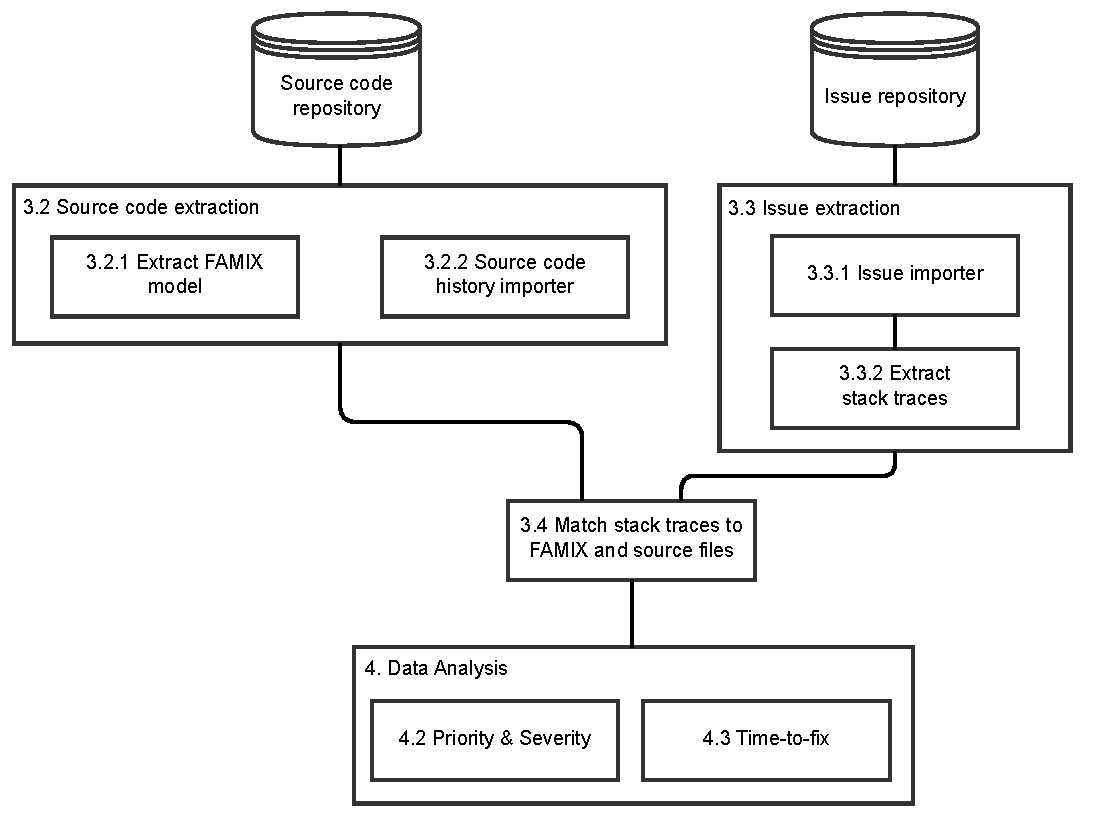
\includegraphics[width=1\textwidth]{img/research_framework.pdf}
	\caption{Overview of the research framework.}
	\label{fig:research_framework}
\end{figure}

The data extraction part makes sure both the source code repository as well as the issue report repository are available for querying. All extractions are performed using the Evolizer framework \cite{Gall2009}, which is a plugin for the Eclipse IDE. Evolizer is a platform for mining software artifact repositories into models. Also, Evolizer is extended to support stack trace extraction and matching. The source code for this extension is available.

The source code extraction consists of generating a model of the source code and the source code repository. The issue reports are extracted from the issue repository into another model, after which stack traces are extracted from these issues. Finally, both the source code model, the source code repository model and the issue model are linked. Based on this data set, the analysis of Chapter \ref{cha:data_analysis} can be performed. In this analysis, two low-level metrics are used: lines of code, and time-to-fix. Both metrics are discussed in Section \ref{sec:low_level_metrics}.

% section overview (end)
\section{Source code extraction} % (fold)
\label{sec:source_code_extraction}
The source code of a project under investigation is extracted from the source code repository in two ways:

\begin{enumerate}
	\item Extraction of the source code into a language independent meta-model that describes the static structure of the source code (Section~\ref{sub:famix_model_extraction})
	\item Extraction of the complete source code repository into a meta-model (Section~\ref{sub:source_code_history_importer})
\end{enumerate} 

\subsection{FAMIX model extraction} % (fold)
\label{sub:famix_model_extraction}
The FAMIX meta-model \cite{Tichelaar2000,Tichelaar2001} is a language independent representation of the static structure of the source code of a project. Figure~\ref{fig:evolizer_class_diagram} depicts the class hierarchy of the FAMIX model as implemented in Evolizer. 

\texttt{AbstractFamixObject} is the base class for FAMIX entities and associations between FAMIX entities. A FAMIX entity represents either a package, class or method. It can also represent a \texttt{FamixVariable}, which represents class attributes, local variables, and formal parameters. Relations between these entities are represented by \texttt{FamixAssociation}s, which are for example casts, invocations or inheritance between entities.

\begin{figure}[!ht]
	\centering
		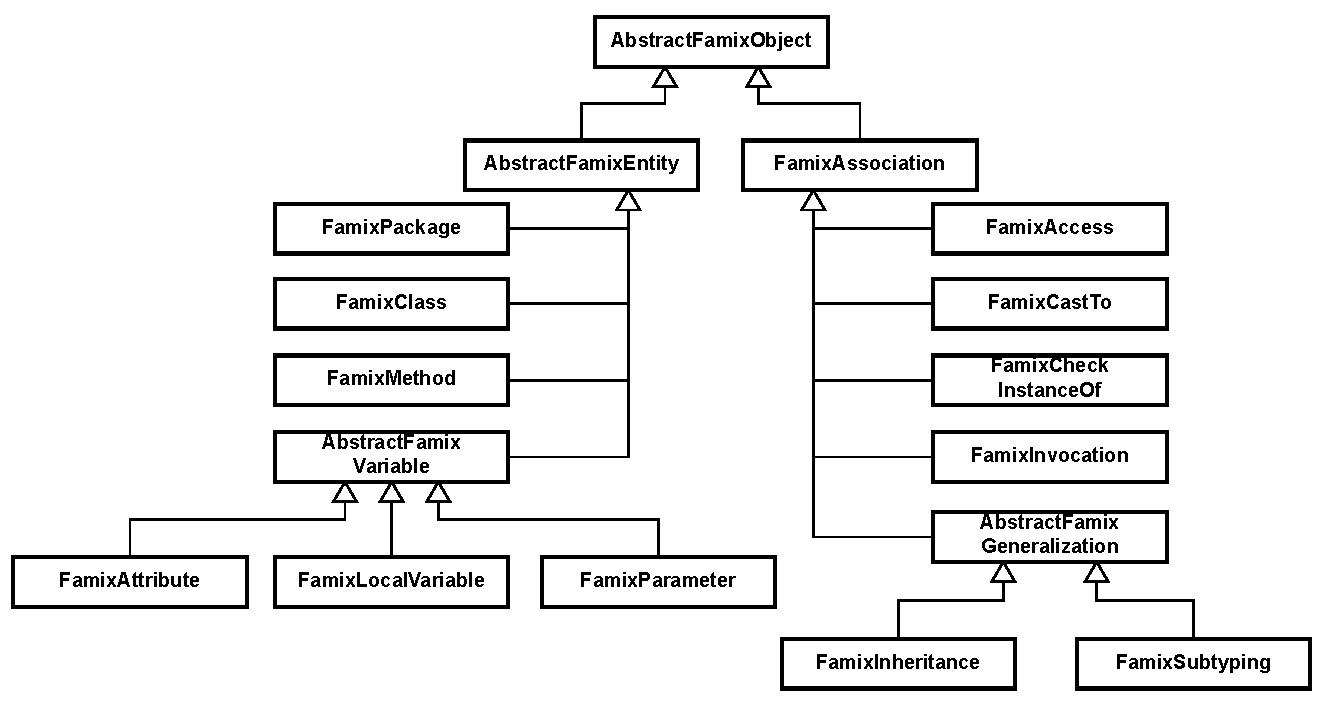
\includegraphics[width=1\textwidth]{img/FAMIX_object_model.pdf}
	\caption{Implementation of the FAMIX meta-model in Evolizer.}
	\label{fig:evolizer_class_diagram}
\end{figure}

Evolizer is able to extract a FAMIX meta-model from the source code of an Eclipse Java project. Eclipse core libraries (for example \texttt{org.eclipse.jdt.core}) are used to extract the FAMIX model. The extracted model is saved in the Evolizer relational database, where it can be queried using the Evolizer Hibernate\footnote{\url{http://www.hibernate.org/}} model or via plain SQL queries. 

Evolizer also offers several metrics, such as number of methods of a class, lines of code of a class, or cyclomatic complexity \cite{McCabe1976}. For some metrics, such as lines of code, it is necessary to have a model of the actual source files, which are part of the source code history. The extraction of this model is detailed in Section~\ref{sub:source_code_history_importer}.
% subsubsection famix_model_extraction (end)

\subsection{Source code history importer} % (fold)
\label{sub:source_code_history_importer}
The source code repository is also extracted to a meta-model, containing versioned files, revisions, branches, releases, et cetera \cite{Fischer}. Figure~\ref{fig:source_code_repository_metamodel} shows a simplified depiction of the source code history meta-model. Central in this model is a \texttt{VersionedFile}, which is a specialised implementation of \texttt{File} that is, of course, versioned. Each versioned file has one or more revisions. A revision is linked to the source code content for that specific revision. The modification report states the commit message for that revision. As can be seen, the meta-model for the source code repository is heavily inspired by CVS like SCM systems. 

\begin{figure}[!ht]
	\centering
		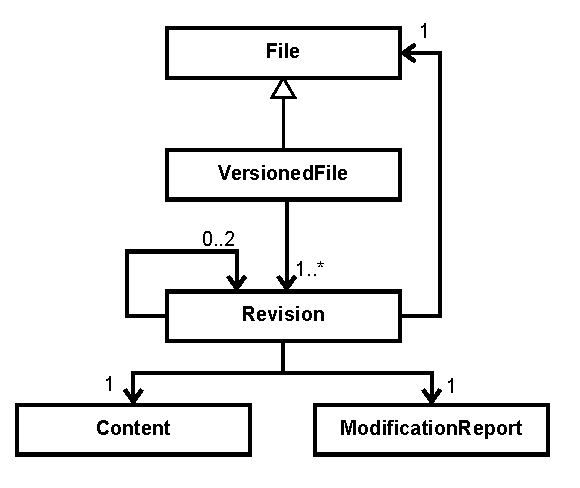
\includegraphics[width=0.5\textwidth]{img/version_history_model.pdf}
	\caption{Source code repository history meta-model.}
	\label{fig:source_code_repository_metamodel}
\end{figure}

Evolizer imports a complete source code repository history into its database, including the contents of all file revisions. In the case of a CVS repository, at first the complete log file is parsed. In this stage, all files under version control are recognized, including all their revisions. After this, the source code contents for all file revisions are read and put into the database, completing the model.
% subsubsection source_code_history_importer (end)
 
% subsection source_code_extraction (end)

\section{Issue report extraction} % (fold)
\label{sub:issue_report_extraction}
Next to the source code repository, Evolizer is also used to extract the issue repository. After the complete repository is extracted, all issue comments are examined for stack traces.

\subsection{Issue repository importer} % (fold)
\label{sub:issue_importer}
Figure~\ref{fig:issue_repo_metamodel} shows a partial representation of the issue meta-model. Each bug repository is split into several levels, starting at a global classification, down to products and specific components of that products. An issue has several properties, such as status, priority, severity and assigned milestone. Each issue can have several comments that form the discussion for that bug report. Also, the history of a bug, such as fixing or closing a bug, (re)assigning a developer, changing priority, et cetera, is captured as activities. 

\begin{figure}[!ht]
	\centering
		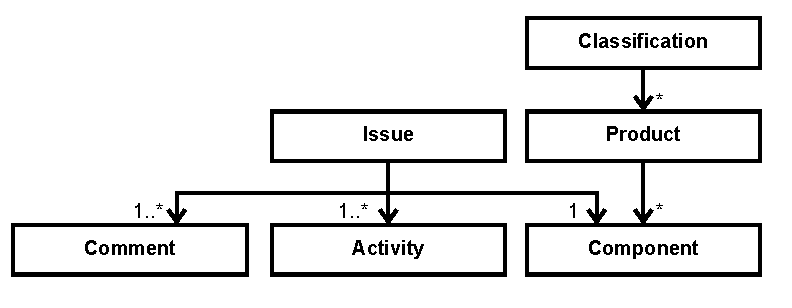
\includegraphics[width=0.7\textwidth]{img/issue-model.pdf}
	\caption{Issue repository meta-model.}
	\label{fig:issue_repo_metamodel}
\end{figure}

Evolizer is able to convert Bugzilla bug repositories to this meta-model. It is possible to extract a complete bug repository or a specific range of bug reports. In order to only extract certain bug reports, for example for a specific product only, Evolizer was extended to be able to enter a comma separated list of bug IDs to import. All bugs are read from Bugzilla in a XML format and parsed by Evolizer using a SAX2\footnote{\url{http://www.saxproject.org/}} parser. After this, the activities of a bug report are parsed. These activities are only available in HTML format, so a HTML parser was used to extract this information.

\subsubsection{Issues} % (fold)
When parsing Bugzilla data using the XML parser, several issues were found\footnote{See Appendix~\ref{cha:bugzilla_importer_xml_parser_issues} for more details.}. These issues were mitigated by correctly implementing the XML importer. Also, some other bugs in the state machine were fixed, such as validating the Bugzilla XML to the correct Document Type Definition. Finally, functionality was added to import bug reports multiple times, without resulting in duplicate data in the Evolizer database.
% paragraph issues (end)
% subsubsection issue_importer (end)

\subsection{Stack trace extraction} % (fold)
\label{sub:stack_trace_extraction}
After all bug report comments are imported, a subsequent pass is performed in order to extract all stack traces from these comments. A stack trace consists of a number of stack trace frames, which are represented by lines in a stack trace. A typical Java stack trace looks like this:

{\small
\begin{verbatim}
	java.lang.ArrayIndexOutOfBoundsException: 2048 	
	at org.eclipse.jdt.internal.core.DiskIndex.readStreamInt(DiskIndex.java:48)
	at org.eclipse.jdt.internal.core.DiskIndex.readHeader(DiskIndex.java:779)
	at org.eclipse.jdt.internal.core.DiskIndex.initialize(DiskIndex.java:379)
	...
	at org.eclipse.core.internal.jobs.Worker.run(Worker.java:48)
\end{verbatim}
}

Complete stack traces are extracted from bug report comments using a regular expression matching on `...Exception' and multiple parts starting with `at' (representing the stack frames):

{\small
\begin{verbatim}
	(.+Exception[^\\n]+(\\s+at\\s?.+)+)+
\end{verbatim}
}

\begin{sloppypar}
Each stack trace frame consists of a qualified name (\texttt{org.eclipse.jdt.internal.core.DiskIndex.readStreamInt}), a source file (\texttt{DiskIndex.java}) and a line number (48)\footnote{\url{http://docs.oracle.com/javase/1.5.0/docs/api/java/lang/StackTraceElement.html}}. The qualified name can subsequently be split into a package name, class name and a method name. 
\end{sloppypar}

Each stack trace frame was parsed using the following regular expression:
{\small
\begin{verbatim}
	((([a-zA-Z0-9\\$]+)\\.)*)(([a-zA-Z0-9\\$]+)\\.([a-zA-Z0-9\\$]+))(\\((.+):(.+)\\))
\end{verbatim}
}

In order to mine all stack traces, first all complete stack traces are extracted from the already imported bug reports. Each bug report can have multiple comments, which in turn can have multiple stack traces. After this, a subsequent pass is performed to parse all stack trace call stacks, again using a regular expression. Each stack trace frame is split into a package name, class name, method name, file name and line number.

\begin{figure}[!ht]
	\centering
		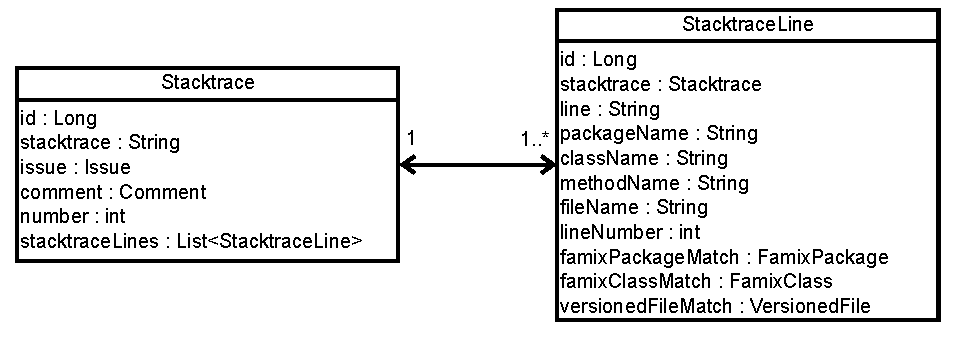
\includegraphics[width=0.8\textwidth]{img/stacktracemodel.pdf}
	\caption{Stack trace model class diagram.}
	\label{fig:stacktrace_model}
\end{figure}

In order to be able to parse and persist all stack traces and corresponding stack frames from the bug repository, Evolizer and its associated object model have been extended. The corresponding class diagram is shown in Figure~\ref{fig:stacktrace_model}.
% subsubsection stack_trace_extraction (end)

% subsection issue_report_extraction (end)

\section{Stack trace extraction and mapping} % (fold)
\label{sec:stack_trace_extraction_and_mapping}
In this stage of data gathering, a FAMIX meta-model, source code repository meta-model, and an issue repository meta-model extended with stack traces are  available. Using the stack traces found, all these models can be linked. For this, each stack trace line will be matched with a FAMIX package, FAMIX class and a versioned file. The resulting overall model is depicted in Figure~\ref{fig:complete_meta_model}.

\begin{figure}[!ht]
	\centering
		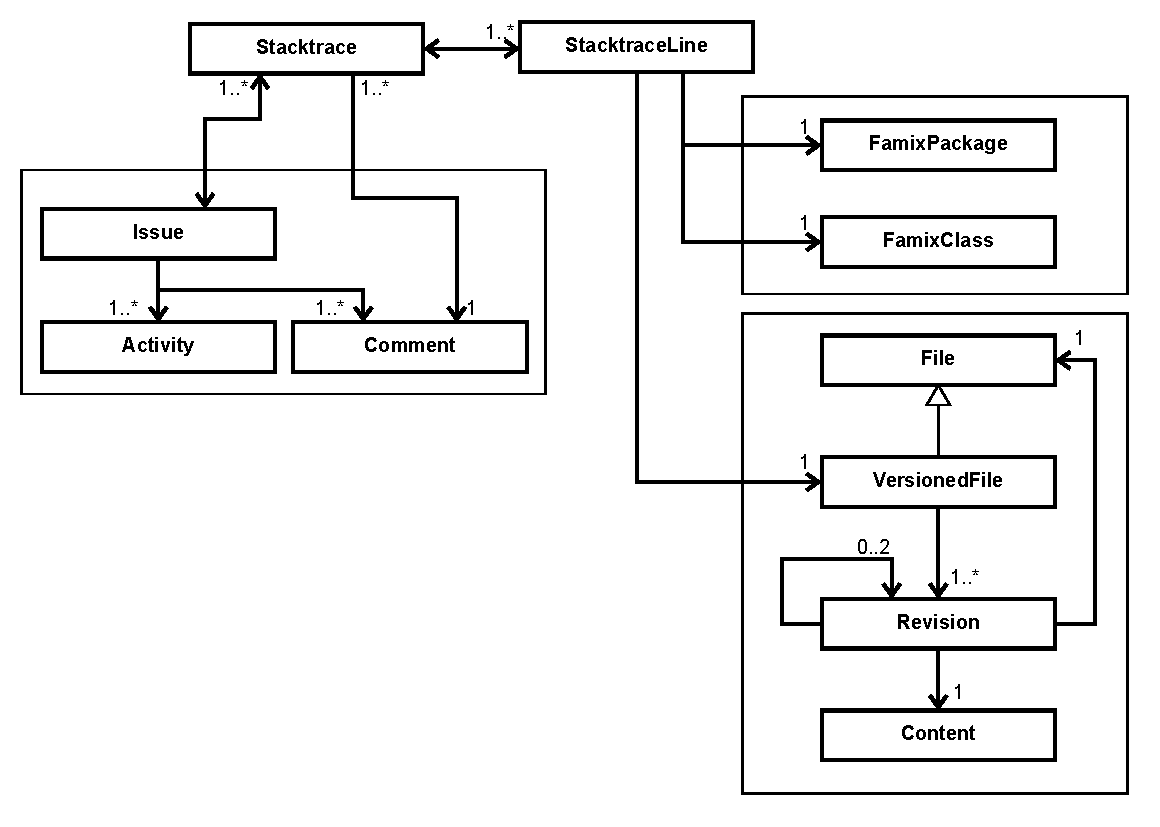
\includegraphics[width=1\textwidth]{img/linked_meta_model.pdf}
	\caption{Complete meta-model for the research framework.}
	\label{fig:complete_meta_model}
\end{figure}

\begin{sloppypar}
FAMIX packages and classes are matched based on string equality. For \texttt{VersionedFile}s, the package and file name from the stack trace line are used to (partly) represent the file path. For example, a package \texttt{org.eclipse.jdt.internal.core} and file name \texttt{DiskIndex.java} is converted to the file path \texttt{org/eclipse/jdt/internal/core/DiskIndex.java}, which in turn is matched to the available \texttt{VersionedFile}s.
\end{sloppypar}

This concludes the extraction of a complete meta-model from the bug report repository and the source code repository, using stack traces to match both models.
% section stack_trace_extraction_and_mapping (end)

\section{Low-level metrics} % (fold)
\label{sec:low_level_metrics}
The metrics used in Chapter \ref{cha:data_analysis} are: lines of code and time-to-fix. This section gives a definition of both these metrics.

\subsection{Lines of code} % (fold)
In order to determine the lines of code of a source file, only the lines which contain actual source code are counted. Comments, import statements, package declarations and empty lines are ignored.

\subsection{Time-to-fix} % (fold)
\label{sub:time_to_fix}
Only issue reports that have resolution \textsc{fixed} and status \textsc{verified} are considered to be fixed, and hence have a time-to-fix. Each bug has an activity history, which records changes in bug properties. The time-to-fix is the number of days between the creation date of the issue report and the \emph{latest} activity in which the resolution changed to `fixed'. This way, possible incomplete fixes are ignored.
% subsection time_to_fix (end)
% section low_level_metrics (end)

% chapter research_framework (end)

%!TEX root = thesis.tex

\chapter{Approach} % (fold)
\label{cha:data_analysis}
This chapter describes the approach to perform the analysis on the data sets generated using the research framework of Chapter~\ref{cha:research_framework}, in order to investigate our research questions and hypothesis.

\section{Overview} % (fold)
\label{sec:overview}
Section~\ref{sec:statistical_tests} briefly describes the statistical tests used to analyse the data. Sections \ref{sec:analysis:priority_and_severity} and \ref{sec:analysis:time_to_fix} describe how to gather the relevant data using the research framework and how to evaluate the hypotheses using statistical tests.
% section overview (end)

\section{Statistical tests} % (fold)
\label{sec:statistical_tests}
Several statistical tests can be used to investigate the hypotheses of this thesis. This section describes the tests that are actually used in Chapters \ref{cha:results_priority_and_severity} and \ref{cha:results_time_to_fix}. To execute the statistical tests, the R language and environment for statistical computing and graphics\footnote{\url{http://www.r-project.org/}} is used.

The statistical significance of each test result is indicated using stars. The significance levels $\alpha$ used in this thesis are summarised in Table~\ref{tab:sig_levels}:

\begin{table}[!ht]\footnotesize
	\centering
	\begin{tabular}{lll}
		\toprule
		$\alpha$ \\
		\midrule
		0.05 & * & significant\\
		0.01 & ** & highly significant\\
		0.001 & *** & extremely significant\\
		\bottomrule
	\end{tabular} 
	\caption{Significance levels used in this thesis.}
	\label{tab:sig_levels}
\end{table}

\subsection{D'Agostino Omnibus $K^2$ normality test} % (fold)
\label{sub:d_agostino_normality_test}
In order to choose a suiting statistical test for data, it is often needed to determine whether the data under investigation is sampled from a Gaussian distribution. Next to a visual inspection (using a histogram, density graph or QQ-plot), the D'Agostino Omnibus $K^2$ test \cite{D'Agostino1971,D'agostinoR.B.andBelangerA.andD'AgostinoJr1990} is used. The null hypothesis $H_0$ for this Omnibus test is: the data is sampled from a Gaussian distribution.

The D'Agostino Omnibus test uses the skewness $\sqrt{b_1}$ and kurtosis $b_2$  of a data set to quantify the similarity with a Gaussian distribution:

\begin{equation}
	K^2 = (Z(\sqrt{b_1}))^2 + (Z(b_2))^2
\end{equation}

The $Z$-function is used to transform the values of skewness and kurtosis. A detailed calculation can be found in \cite{D'Agostino1971}. The distribution of $K^2$ is approximately a chi-squared distribution with two degrees of freedom. With this, a $p$-value can be calculated. 

When the $p$-value is less than the significance level $\alpha$, the null hypothesis of normality is rejected.

% subsection d_agostino_normality_test (end)

\subsection{Chi-squared test} % (fold)
\label{sub:chi_squared_test}
Pearson's chi-squared test \cite{Pearson1900} is used as a test of independence between two categorical variables. The null hypothesis $H_0$ states: there is no association between the two variables.

With the first variable having $r$ categories, and the second variable having $c$, a $r \times c$ contingency table can be constructed, containing the count values observed. Based on these count values (and their totals), the expected count value $E$ is determined by:

\begin{equation}
	E_{i,j}=\frac{(\sum_{n_c=1}^c O_{i,n_c}) (\sum_{n_r=1}^r O_{n_r,j})}{N} 
\end{equation}

where $O$ is the observed count, $n$ the number of cells and $N$ the sum of all cell values. The test statistic $\chi^2$ is defined as:

\begin{equation}
\chi^2 = \sum_{i=1}^{r} \sum_{j=1}^{c} {(O_{i,j} - E_{i,j})^2 \over E_{i,j}} 
\end{equation}

The distribution of $\chi^2$ is approximately a chi-squared distribution with $(r-1)(c-1)$ degrees of freedom. With this, the $p$-value can be calculated. When the $p$-value is less than the significance level $\alpha$, the null hypothesis of `there is no association between the two variables' is rejected.

The validity of a chi-squared test depends on the sample size of the whole dataset and the expected theoretical cell counts. Cochran \cite{Cochran1954} states that, with respect to the expected cell counts, the chi-square approximation is adequate when the expected count is 5 or more in 80\% of the cells and no cells have an expected count less than one.

To investigate which combination(s) of variables has a high impact on the $\chi^2$ statistic, one can take into account the contribution of each $(O-E)^2/E$ value to the overall chi-squared statistic. As a rule of thumb, when $(O-E)^2/E > 4$, that particular association is significantly different.

% subsection chi_squared_test (end)

\subsection{Wilcoxon Rank Sum test} % (fold)
\label{sub:wilcoxon_rank_sum_test}
Nonparametric tests are used on measures of central tendency (such as the median), when the distribution of the data set is not normal. When distributions are similarly shaped, the (Mann-Whitney) Wilcoxon Rank Sum test \cite{Wilcoxon1945, Mann1947} can be used to determine if there is a shift in location of this central tendency.

The Wilcoxon Rank Sum test assumes the two independent continuous random samples $X$ and $Y$ have a measurement scale that is at least ordinal. Also, the distributions of $X$ and $Y$ are identically shaped, and only have a shift in location $\theta$. The null hypothesis $H_0$ of the Wilcoxon Rank Sum test states that the median value $M$ of $X$ and $Y$ are the same: $M_x = M_y$. Three possible alternative hypothesis are:

\begin{enumerate}
	\item $H_a$ : $M_x \neq M_y$
	\item $H_a$ : $M_x < M_y$
	\item $H_a$ : $M_x > M_y$
\end{enumerate}

The algorithm for the Wilcoxon Rank Sum test is described in detail in the original paper \cite{Wilcoxon1945} from Frank Wilxocon.  When the $p$-value is less than the significance level $\alpha$, the null hypothesis that states the median values of the data sets are equal, is rejected.

In order to investigate the sign of the shift in location $\theta$ of the median, let's state that $F(x)$ and $G(x)$ are the distribution functions of $X$ and $Y$ respectively. The shift in location $\theta$ is now defined by:

\begin{equation}
	G(x) = F(x + \theta) \mbox{ for all } x
\end{equation}	

% subsection wilcoxon_rank_sum_test (end)

\subsection{Kendall tau-b rank correlation coefficient} % (fold)
\label{sub:kendall_tau_b_rank_correlation_coefficient}
Kendall's tau test \cite{Kendall1938} can be used to test a possible association between two categorical random variables $X$ and $Y$, and does not rely on the distributions of $X$ and $Y$. The null hypothesis $H_0$ states: there is no association between $X$ and $Y$. 

The original algorithm from Kendall does not account for \emph{ties}. A pair is tied if for ${(x_i, y_i), (x_j, y_j)}$, $x_i = x_j$ or $y_i = y_j$. In order to make adjustments for these ties, the tau-b variant \cite{Adler1957} of Kendall's test is used.

The $\tau_B$ coefficient will be in the range $-1 \leq \tau_B \leq 1$ and indicates the strength and sign of the relationship between the two variables $X$ and $Y$. Since only the strength of the relationship is of interest, the absolute value of $\tau_B$ is used. Table~\ref{tab:tau_correlation} shows how to interpret the $\tau_B$ coefficient in terms of correlation.

\begin{table}[!ht]\footnotesize
	\centering
	\begin{tabular}{ll}
		\toprule
		Value & Type \\
		\midrule
		$\tau_B = 0$ & No correlation \\
		$0 < \tau_B < 0.5$ & Weak correlation \\
		$0.5 \leq \tau_B \leq 0.7$ & Substantial correlation \\
		$0.7 < \tau_B < 1$ & Strong correlation \\
		$\tau_B = 1$ & Perfect correlation \\
		\bottomrule
	\end{tabular} 
	\caption{Interpretation of correlation coefficient}
	\label{tab:tau_correlation}
\end{table}

The $p$-value can again be used to accept or reject the null hypothesis. When the $p$-value is less than the significance level $\alpha$, we reject that there is no association between $X$ and $Y$. 
% subsection kendall_tau_b_rank_correlation_coefficient (end)

% section statistical_tests (end)

\section{Priority and severity} % (fold)
\label{sec:analysis:priority_and_severity}

This section describes the methodology used to answer research question R1:

\vspace{\baselineskip}
\questiona{}
\vspace{\baselineskip}

For each investigation of the hypotheses of R1, we describe how the data sets should be composed and how to subsequently analyse these data sets.

\subsection{Analysis of priority and severity related to the presence of a stack trace} % (fold)
\label{sub:da:analysis_of_priority_and_severity_related_to_the_presence_of_a_stack_trace}
When a stack trace is present, a bug triager might be able to identify the location of a bug in source code more easily. This way, it might be also easier to assign a representative priority and severity to the bug report (i.e., less bugs with default priority and severity). This section describes the methodology to investigate hypotheses H1.1 and H1.2:

\vspace{\baselineskip}
\hypaa{}

\vspace{\baselineskip}
\hypab{}

\vspace{\baselineskip}

\subsubsection{Composition of data set}
All issue reports are split into two groups: issues with and issues without a stack trace. For each of these groups, the number of issue reports for every priority (and severity) is counted.

\subsubsection{Analysis}
To test whether there is an association between priority and presence of a stack trace (and between severity and presence of a stack trace), a statistical test of independence is performed. The null hypothesis $H_0$ of such a test states `there is no association between two variables', where the alternative hypothesis $H_a$ states `the two variables are associated'. Since the data under test is categorical data (i.e., count data), a chi-squared test is used.

For priority, a $p \times c$ contingency table is constructed, where $p$ is the number of priorities and $c$ the two groups (issue reports with and without a stack trace). Similar, for severity a $s \times c$ contingency table is constructed.

For these contingency tables, the $\chi^2$ metric is calculated and the validity of the outcome is checked using the sample size of the whole dataset and the expected theoretical cell counts.

Based on the $p$-value of the $\chi^2$ test, it is determined whether the result is statistically significant. If this turns out to be true, the null hypothesis is rejected, giving evidence that there is an association between the variables.

In order to investigate which cell(s) in the contingency table contribute significantly to the association, the contribution of each $(O-E)^2/E$ value to the overall chi-squared statistic is considered. 
% subsection analysis_of_priority_and_severity_related_to_the_presence_of_a_stack_trace (end)

\subsection{Analysis of priority and severity related to package size} % (fold)
\label{sub:da:analysis_of_priority_and_severity_related_to_package_size}
When one or more stack traces are present in comments of a bug report, it is possible to relate each bug report to one or more source packages mentioned in the stack frames. A larger package size might point to a more important subsystem of the software, hence to a higher priority or severity of a bug. This section describes the methodology to investigate hypotheses H1.3 and H1.4:

\vspace{\baselineskip}
\hypac{}

\vspace{\baselineskip}
\hypad{}

\vspace{\baselineskip}

The \emph{size} of a package is not bound to a single evident definition. Three possible definitions are investigated in this thesis:

\begin{enumerate*}
	\item number of classes (NOC)
	\item total lines of code of associated classes (SUMLOC)
	\item (arithmetic) mean of lines of code of associated classes (AVGLOC)
\end{enumerate*}

\subsubsection{Composition of data set}
For each bug report with a stack trace, all associated packages are determined, which in turn have the above mentioned size metrics (when their associated classes can be found in the source code repository). A bug report can have multiple stack traces, and a stack trace can have multiple associated packages. This results in a list of pairs \emph{(report, package)}. 

It is possible that the same stack trace is mentioned multiple times in a bug report (for example in a quoted message). Also, a package can be mentioned multiple times in a stack trace. In order to make sure these duplicates do not affect the statistics, only unique pairs \emph{(report, package)} are considered.

\subsubsection{Analysis}
In order to investigate whether there is a relation between priority (or severity) and package size, a pairwise comparison of the median values of each data set is made. For priority, P1 and P2 are compared, P2 and P3, et cetera. For severity, `blocker' and `critical' are compared, `critical' and `major', et cetera. The median values of each data set are compared to show whether or not these median values increase when the priority (or severity) increases. 

First, the data sets are visually inspected using box plots for each priority and severity, showing the distribution of the package size. Also, some descriptive statistics of package size, such as minimum, maximum, mean and median, are inspected.

Next, the D'Agostino normality test is applied to determine if the distribution of the data sets is normal. Also, by visually inspecting the density graph of all data sets, it is determined whether the distributions of the data sets are similar shaped.

If the data sets are not normal distributed, but the distributions of the data sets are similar shaped, the Wilcoxon Rank Sum test can be used to compare the medians of the data sets. Otherwise, another suitable statistical test should be used. The null hypothesis $H_0$ for the Wilcoxon test is $M_1 = M_2$, where $M_i$ is the median of group $i$. In other words, the median values of the two data sets do not differ. The alternative one-sided hypothesis $H_a$ is $M_1 > M_2$. This alternative hypothesis of the Wilcoxon Rank Sum test corresponds to the hypotheses that are investigated in this section.

Based on the $p$-value of the Wilcoxon Rank Sum test, it is determined whether the result is statistically significant. If this turns out to be true, the null hypothesis is rejected, giving evidence there is a shift $\theta$ in medians. Whether the location shift corresponds with the chosen alternative hypothesis is determined by the sign of $\theta$.

% subsection analysis_of_priority_and_severity_related_to_package_size (end)

\subsection{Analysis of priority and severity related to class size} % (fold)
\label{sub:analysis_of_priority_and_severity_related_to_class_size}
Lines of code of a class is often used as one of the most important metrics for class size. Other metrics, such as number of methods, fan-in and fan-out are sometimes also considered. This section describes the methodology to investigate if there is a relation between the priority (and the severity) of a bug report and the lines of code of the corresponding classes listed in the stack traces of that bug report. This corresponds to hypotheses H1.5 and H1.6:

\vspace{\baselineskip}
\hypae{}

\vspace{\baselineskip}
\hypaf{}

\vspace{\baselineskip}

\subsubsection{Composition of data set}
For each bug report with a stack trace, all associated classes are determined, which all have a lines of code metric (when the source code of the class can be found in the source code repository). A bug report can have multiple stack traces, and a stack trace can have multiple associated classes. This results in a list of pairs \emph{(report, class)}. It is possible that the same stack trace is mentioned multiple times in a bug report (for example in a quoted message). Also, a class can be mentioned multiple times in a stack trace. 

In order to make sure these duplicates do not affect the statistics, only \emph{unique} pairs \emph{(report, class)} are considered. The length of a stack trace is not taken into consideration: all unique pairs are used, creating as many relations between data sets as possible.

\subsubsection{Analysis}
In order to investigate whether there is a relation between priority (or severity) and class size, a pairwise comparison of the median values of each data set is made. For this, the same analysis as described in Section~\ref{sub:da:analysis_of_priority_and_severity_related_to_package_size} is applied, again using the Wilcoxon Rank Sum test. 

% subsection analysis_of_priority_and_severity_related_to_class_size (end)

% section priority_and_severity (end)

\section{Time-to-fix} % (fold)
\label{sec:analysis:time_to_fix}
This section describes the methodology used to answer research question R2:

\vspace{\baselineskip}
\questionb{}
\vspace{\baselineskip}

For each investigation of the hypotheses of R2, it is described how the data sets should be composed and how to subsequently analyse these data sets.

\subsection{Analysis of time-to-fix versus presence of stack traces in bug report} % (fold)
\label{sub:da:analysis_of_time_to_fix_versus_presence_of_stack_traces_in_bug_report}
One would expect that the time-to-fix of a bug decreases when a stack trace is present in the bug report, as showed in previous work by Schr\"{o}ter \emph{et al.} \cite{Schroter2010}. With this stack trace, it might be easier to reproduce the bug or to know where to look in the source code. This section describes the methodology used to hypothesis H2.1:

\vspace{\baselineskip}
\hypba{}

\subsubsection{Composition of data set}
All bug reports marked with status \textsc{verified} and resolution \textsc{fixed} are split into two groups: 

\begin{enumerate*}
	\item bug reports that include a stack trace in one or more of the comments, and
	\item bug reports that do not include a stack trace.
\end{enumerate*}

For each bug report, the time-to-fix is calculated. All reports with a time-to-fix of $0$ days are removed from the data sets, since these reports probably are only created for administrative reasons.

\subsubsection{Analysis}
In order to investigate if the time-to-fix of a bug decreases when a stack trace is present in the bug report, the median time-to-fix for the data sets with and without stack traces are compared. 

First, some descriptive statistics and a visual representation (box plots) are used to perform a first inspection of the data. Next, the D'Agostino normality test is applied to determine if the distribution of the data sets is normal. Also, by visually inspecting the density graph of all data sets, it is determined whether the distributions of the data sets are similar shaped.

If the data sets are not normally distributed, but the distributions of the data sets are similar shaped, the Wilcoxon Rank Sum test can be used to compare the medians of the data sets. Otherwise, another suitable statistical test should be used. The null hypothesis $H_0$ for the Wilcoxon test is $M_1 = M_2$, where $M_i$ is the median of group $i$. In other words, the median values of the two data sets do not differ. The alternative one-sided hypothesis $H_a$ is $M_1 < M_2$. This alternative hypothesis of the Wilcoxon Rank Sum test corresponds to the hypothesis that is investigated in this section.

Based on the $p$-value of the Wilcoxon Rank Sum test, it is determined whether the result is statistically significant. If this turns out to be true, the null hypothesis is rejected, giving evidence there is a shift $\theta$ in medians. Whether the location shift corresponds with the chosen alternative hypothesis is determined by the sign of $\theta$.
% subsection analysis_of_time_to_fix_versus_presence_of_stack_traces_in_bug_report (end)

\subsection{Analysis of time-to-fix versus stack trace position in comments} % (fold)
\label{sub:da:analysis_of_time_to_fix_versus_stack_trace_position_in_comments}
The previous section investigated if there is evidence for a decrease in time-to-fix when a stack trace is present. This section investigates whether the time-to-fix is positively affected (i.e., decreases) when the stack trace is present in the \emph{first} comment of a bug report. This way, the stack trace is immediately available to the bug traiger, and can therefore be used in the assessment of the bug report. This is formalised in hypothesis H2.2:

\vspace{\baselineskip}
\hypbb{}

\subsubsection{Composition of data set}
Again, all bug reports marked with status \textsc{verified} and resolution \textsc{fixed} are split into two groups: 

\begin{enumerate*}
	\item bug reports with one or more stack traces in the first comment, and
	\item bug reports with one or more stack traces in non-first comment(s).
\end{enumerate*}

For each bug report, the time-to-fix is calculated. All reports with a time-to-fix of $0$ days are removed from the data sets, since these reports probably are only created for administrative reasons.

\subsubsection{Analysis}
The analysis for these data sets equals the analysis as described in Section~\ref{sub:da:analysis_of_time_to_fix_versus_presence_of_stack_traces_in_bug_report}.

% subsection analysis_of_time_to_fix_versus_stack_trace_position_in_comments (end)

\subsection{Correlation analysis between class size and time-to-fix} % (fold)
\label{sub:da:correlation_analysis_between_class_size_and_time_to_fix}
When one or more stack traces are present in comments of a bug report, it is possible to relate each bug report to one or more source classes. A larger class size might point to less understandable code, hence to a higher time-to-fix for a bug. This section shows the methodology used to investigated if there is a relation between class size and time-to-fix of a bug report. This equals hypothesis H2.3:

\vspace{\baselineskip}
\hypbc{}

\subsubsection{Composition of data set}
The total data set contains all classes that are matched to at least \emph{ten} bug reports that have a time-to-fix (i.e., have status \textsc{verified} and resolution \textsc{fixed}). All bug reports with a fix time of 0 days are removed from the data set. For each class, the median time-to-fix of all matching issues is calculated. This results in a data set of (\emph{ttf},\emph{loc}) pairs.

\subsubsection{Analysis}
First, a scatter plot of all data points is used to visualise the possible correlation between time-to-fix and class size. To this scatter plot, a linear regression line and a non-parametric Loess \cite{Cleveland1979,Cleveland1988} regression line are added. Since a Loess regression line is non-parametric, it does not make an assumption about the form of the relationship between time-to-fix and class size. Next to the scatter plot, a box plot for both the median time-to-fix and the lines of code is used to inspect the distribution of these values.

In order to statistically verify if a correlation is present, the Kendall tau-b rank correlation coefficient ($\tau_B$) is calculated. When the $p$-value of the Kendall tau-b test makes that the null hypothesis $H_0$ is rejected, there is evidence that there is association between the median time-to-fix and class size. The $\tau_B$ value then indicates the strength of the correlation, as can be seen in Table~\ref{tab:tau_correlation}.

% subsection correlation_analysis_between_class_size_and_time_to_fix (end)

% section time_to_fix (end)
% chapter data_analysis (end)
% part approach (end)

\part{Results} % (fold)
\label{prt:results}
%!TEX root = thesis.tex

\chapter{Project Selection} % (fold)
\label{cha:project_selection}
This chapter describes the projects selected for the actual study performed in Chapters \ref{cha:results_priority_and_severity} and \ref{cha:results_time_to_fix}. 

\section{Overview} % (fold)
First, the requirements for suitable projects are stated. Next, the projects selected for the study are discussed. In the next chapter, descriptive statistics for the projects are presented, in order to get a more detailed view on the projects.
% section overview (end)

\section{Project requirements} % (fold)
\label{sec:project_requirements}
To expect statistically significant results using the research framework as described in Chapter~\ref{cha:research_framework}, sufficient data needs to be available to perform the investigations of our research questions and hypotheses. 

We expect the number of issue reports that include a stack trace to be around 10\% of the total amount of issue reports, where each bug reports with a stack trace contains on average one stack trace. Also, we expect around 50\% of all issue reports being fixed and verified. With around 5000 issue reports, we expect to have sufficient data for our investigations. Regarding classes and packages, we expect 500 classes to be sufficient. With on average 20 classes per package, this comes down to 25 packages total. 

In short, this comes down to the following requirements for the projects under investigation:

\begin{itemize*}
	\item sufficient issue reports (> 5000)
	\item sufficient issue reports that include a stack trace (> 500)
	\item sufficient issue reports that are fixed and verified (> 2500)
	\item sufficient overall number of stack traces (> 500)
	\item sufficient packages in source code (> 25)
	\item sufficient classes in source code (> 500)
\end{itemize*}

% section project_requirements (end)

\section{Selected projects} % (fold)
\label{sec:selected_projects}
In order to meet the requirements set in the previous section, project with a large issue report history and a high presence of stack traces are needed. With this in mind, the Eclipse project seems to be a solid pick.

Several Eclipse sub-projects are available, of which projects for the Java Development Tools (JDT), which include support for Java building and debugging, are obvious choices. These projects were present in the first release of Eclipse and therefore have a long bug report history. Also, due to the technical nature of the Java development tools projects, sufficient stack traces are to be  expected. The JDT projects have also been extensively used in previous work \cite{Gall2009,Giger2010,Lamkanfi2010,D'Ambros2010,Bettenburg2008a}.

From the JDT projects, JDT Debug\footnote{\url{http://www.eclipse.org/projects/project.php?id=eclipse.jdt.debug}} and JDT Core\footnote{\url{http://www.eclipse.org/projects/project.php?id=eclipse.jdt.core}} seem reasonable first picks.
Table~\ref{tab:project-requirements} shows the required data for JDT Core and JDT Debug. All bug report data comes from the Eclipse bug tracker\footnote{\url{https://bugs.eclipse.org/}}, the source code from the Eclipse CVS repository\footnote{\url{http://dev.eclipse.org/viewcvs/}, CVS has been deprecated at Eclipse, projects are being moved to Git.}. All issue reports from the start of the repository to 13 January 2012 are considered. For source files, tagged revision R3\_7 is used.

\begin{table}[!ht]\footnotesize
	\centering
	\begin{tabular}{lrrr}
		\toprule
		requirement & jdt.debug & jdt.core & overall \\
		\midrule
		issue reports & 7,815 & 13,871 & 21,686\\
		issue reports with stack trace & $\approx$ 681 & $\approx$ 899 & $\approx$ 1,580 \\
		fixed issue reports & 3,286 & 5,446 & 8,732 \\
		packages & 32 & 50 & 82 \\
		classes & 469 & 1,182 & 1,651 \\
		\bottomrule
	\end{tabular} 
	\caption{Project requirements investigation. Number of issues reports with a stack trace is estimated based on a search query in Bugzilla.}
	\label{tab:project-requirements}
\end{table}

As can be seen, all requirements stated in Section~\ref{sec:project_requirements} are met, except for the number of classes for \texttt{jdt.debug}. Since importing bug report repositories and CVS repositories into Evolizer is a lengthy process, \texttt{jdt.debug} and \texttt{jdt.core} will be regarded adequate picks to perform the investigations in this thesis. 

% section selected_projects (end)
% chapter project_selection (end)
%!TEX root = thesis.tex

\chapter{Descriptive statistics} % (fold)
\label{cha:descriptive_statistics}

This chapter describes some high level descriptive statistics about the selected projects for this research, in order to get a more detailed view on the selected projects. These statistics are used as additional information in subsequent chapters. This way, we are able to better interpret the results of our research. 

\section{Overview} % (fold)
At first, some general statistics are presented. Then, a more detailed view is given on statistics on priority, severity, time-to-fix, package size and class size.

For the investigations in this thesis, two Bugzilla bug repositories are used: \texttt{jdt.debug} and \texttt{jdt.core}. All bug reports from the start of the bug tracker (10 October 2001) to 13 January 2012 are used. For the source code, revision R3\_7 from CVS is used. Statistics about the number of bug reports under investigation can be seen in Table~\ref{tab:issues-imported} and Table~\ref{tab:issues-st}. 

Two bug reports from \texttt{jdt.debug} are not imported due to not well-formed XML. From \texttt{jdt.core}, only bug reports with the word `Exception' are imported \footnote{\url{https://bugs.eclipse.org/bugs/buglist.cgi?classification=Eclipse&component=Core&f1=creation_ts&longdesc=exception&longdesc_type=allwordssubstr&o1=lessthaneq&product=JDT&query_format=advanced&v1=2012-01-12&order=bug_id&limit=0}}, since importing takes quite some time and only these bug reports are relevant for the investigation. From CVS, all data is imported.

\section{Overall statistics} % (fold)
Only around 6.5\% of all bug reports contains one or more stack traces. This is quite low, compared to the 11\% found by Anvik \emph{et al.} \cite{Anvik2006}. For \texttt{jdt.debug}, one out of four reports that contain a stack trace can be matched to both the FAMIX model and source code (see Table~\ref{tab:issues-st}). For \texttt{jdt.core}, this number is a bit higher: six out of ten can be matched to both the FAMIX model and the source code. Overall, a mere 1.9\% of the bug reports for \texttt{jdt.debug} and 3.5\% of the imported bug reports for \texttt{jdt.core} can be matched to both the FAMIX model and the source code.

\begin{table}[!ht]\footnotesize
	\centering
	\begin{tabular}{lrrrrrr}
		\toprule
		& jdt.debug && jdt.core && overall & \\
		\midrule
		Total reports in bug tracker & 7,815 && 13,871 && 21,686 & \\
		Reports imported in Evolizer & 7,813 && 3,692 && 11,505 & \\
		\midrule
		Reports with > 0 stack traces & 598 & 7.7\% & 816 & 5.9\% & 1,414 & 6.5\% \\
		Match to FAMIX model & 146 & 1.9\% & 484 & 3.5\% & 630 & 2.9\% \\
		Match to source model & 155 & 2.0\% & 493 & 3.6\% & 648 & 3.0\% \\
		Match to FAMIX and source model & 146 & 1.9\% & 481 & 3.5\% & 627 & 2.9\% \\
		\bottomrule
	\end{tabular} 
	\caption{Bug report statistics.}
	\label{tab:issues-imported}
\end{table}

\begin{table}[!ht]\footnotesize
	\centering
	\begin{tabular}{lrrrrrr}
		\toprule
		& jdt.debug && jdt.core && overall & \\
		\midrule
		Reports with > 0 stack traces & 598 && 816 && 1,414 & \\
		\midrule
		Match to FAMIX model & 146 & 24.4\% & 484 & 59.3\% & 630 & 44.6\% \\
		Match to source model & 155 & 25.9\% & 493 & 60.4\% & 648 & 45.8\% \\
		Match to FAMIX and source model & 146 & 24.4\% & 481 & 58.9\% & 627 & 44.3\% \\
		\bottomrule
	\end{tabular} 
	\caption{Bug reports with at least one stack trace in the associated comments.}
	\label{tab:issues-st}
\end{table}

\begin{table}[!ht]\footnotesize
	\centering
	\begin{tabular}{lrrrrrr}
		\toprule
		& jdt.debug && jdt.core && overall & \\
		\midrule
		Total stack traces & 941 && 1,158 && 2,099 & \\
		\midrule
		Match to FAMIX model & 241 & 25.6\% & 643 & 55.5\% & 884 & 42.1\% \\
		Match to source model & 253 & 26.9\% & 655 & 56.6\% & 908 & 43.3\% \\
		Match to FAMIX and source model & 241 & 26.6\% & 640 & 55.3\% & 881 & 42.0\% \\
		\bottomrule
	\end{tabular} 
	\caption{Stack trace statistics.}
	\label{tab:st}
\end{table}

In all imported bug reports, a total number of 2,099 stack traces is found, as can be seen in Table~\ref{tab:st}. For \texttt{jdt.debug}, one in four stack traces can be matched to both the FAMIX model and the source code. For \texttt{jdt.core}, this is applicable to around one in two stack traces. Overall, around 40\% of all stack traces can be matched to the FAMIX model and source code.

The low percentage of bug reports with an actual stack trace was expected based on the preliminary investigation in Section~\ref{sec:selected_projects}. However, the number of matches with the FAMIX meta-model and the source code meta-model are below expectation.

\section{Priority} % (fold)
\label{sec:priority}
Every bug report in the Eclipse bug repository has a priority between 1 and 5, where P1 is a high priority bug report and P5 a low priority bug report. Table~\ref{tab:priority} shows the distribution of all bug reports, including a breakdown into bugs reports with and without a stack trace. The same data is also visualised in Figure~\ref{fig:priority}, showing a box plot with and without outliers. As can be seen, the time-to-fix distribution has a long tail with many outliers.

Overall, 90\% of all bug reports have priority P3, which is the default priority in the Eclipse bug repository. Around 7\% of all bugs have a higher priority, a bit more than 2\% have a lower priority. 

When all bug reports are split into two groups, with and without stack traces, a small shift can be noticed in priorities. Whether or not there is a relation between priority and the presence of a stack trace is investigated in Section~\ref{sec:analysis_of_priority_and_severity_related_to_lines_of_code}.

\begin{table}[!ht]\footnotesize
	\centering
	\begin{tabular}{lrrrrrr}
		\toprule
		& jdt.debug && jdt.core && overall & \\
		\midrule
		All bug reports & 7,815 && 13,871 && 21,686 & \\
		\midrule
		P1 (high) & 425 & 5.4\% & 174 & 1.3\% & 599 & 2.8\%\\
		P2 & 676 & 8.7\% & 366 & 2.6\% & 1,042 & 4.8\%\\
		P3 (default) & 6,552 & 83.8\% & 12,959 & 93.4\% & 19,511 & 90.0\%\\
		P4 & 148 & 1.9\% & 79 & 0.6\% & 227 & 1.0\%\\
		P5 (low) & 14 & 0.2\% & 293 & 2.1\% & 307 & 1.4\%\\
		\\
		\midrule
		Bug reports without stack trace & 7,215 && 13,055 && 20,270 \\
		\midrule
		P1 (high) & 380 & 5.3\% & 153 & 1.2\% & 533 & 2.6\%\\
		P2 & 623 & 8.6\% & 344 & 2.6\% & 967 & 4.8\%\\
		P3 (default) & 6,056 & 83.9\% & 6,056 & 93.4\% & 18,246 & 90.0\%\\
		P4 & 142 & 2.0\% & 78 & 0.6\% & 220 & 1.1\%\\
		P5 (low) & 14 & 0.2\% & 290 & 2.2\% & 304 & 1.5\%\\
		\\
		\midrule
		Bug reports with stack trace & 598 && 816 && 1,414 \\
		\midrule
		P1 (high) & 45 & 7.5\% & 21 & 2.6\% & 66 & 4.7\%\\
		P2 & 51 & 8.5\% & 22 & 2.7\% & 73 & 5.2\%\\
		P3 (default) & 496 & 82.9\% & 769 & 94.2\% & 1,265 & 89.5\%\\
		P4 & 6 & 1.0\% & 1 & 0.1\% & 7 & 0.5\%\\
		P5 (low) & 0 & 0.0\% & 3 & 0.4\% & 3 & 0.2\%\\
		\bottomrule
	\end{tabular} 
	\caption{Statistics for priority.}
	\label{tab:priority}
\end{table}
 
\begin{figure}[!ht]
	\centering
		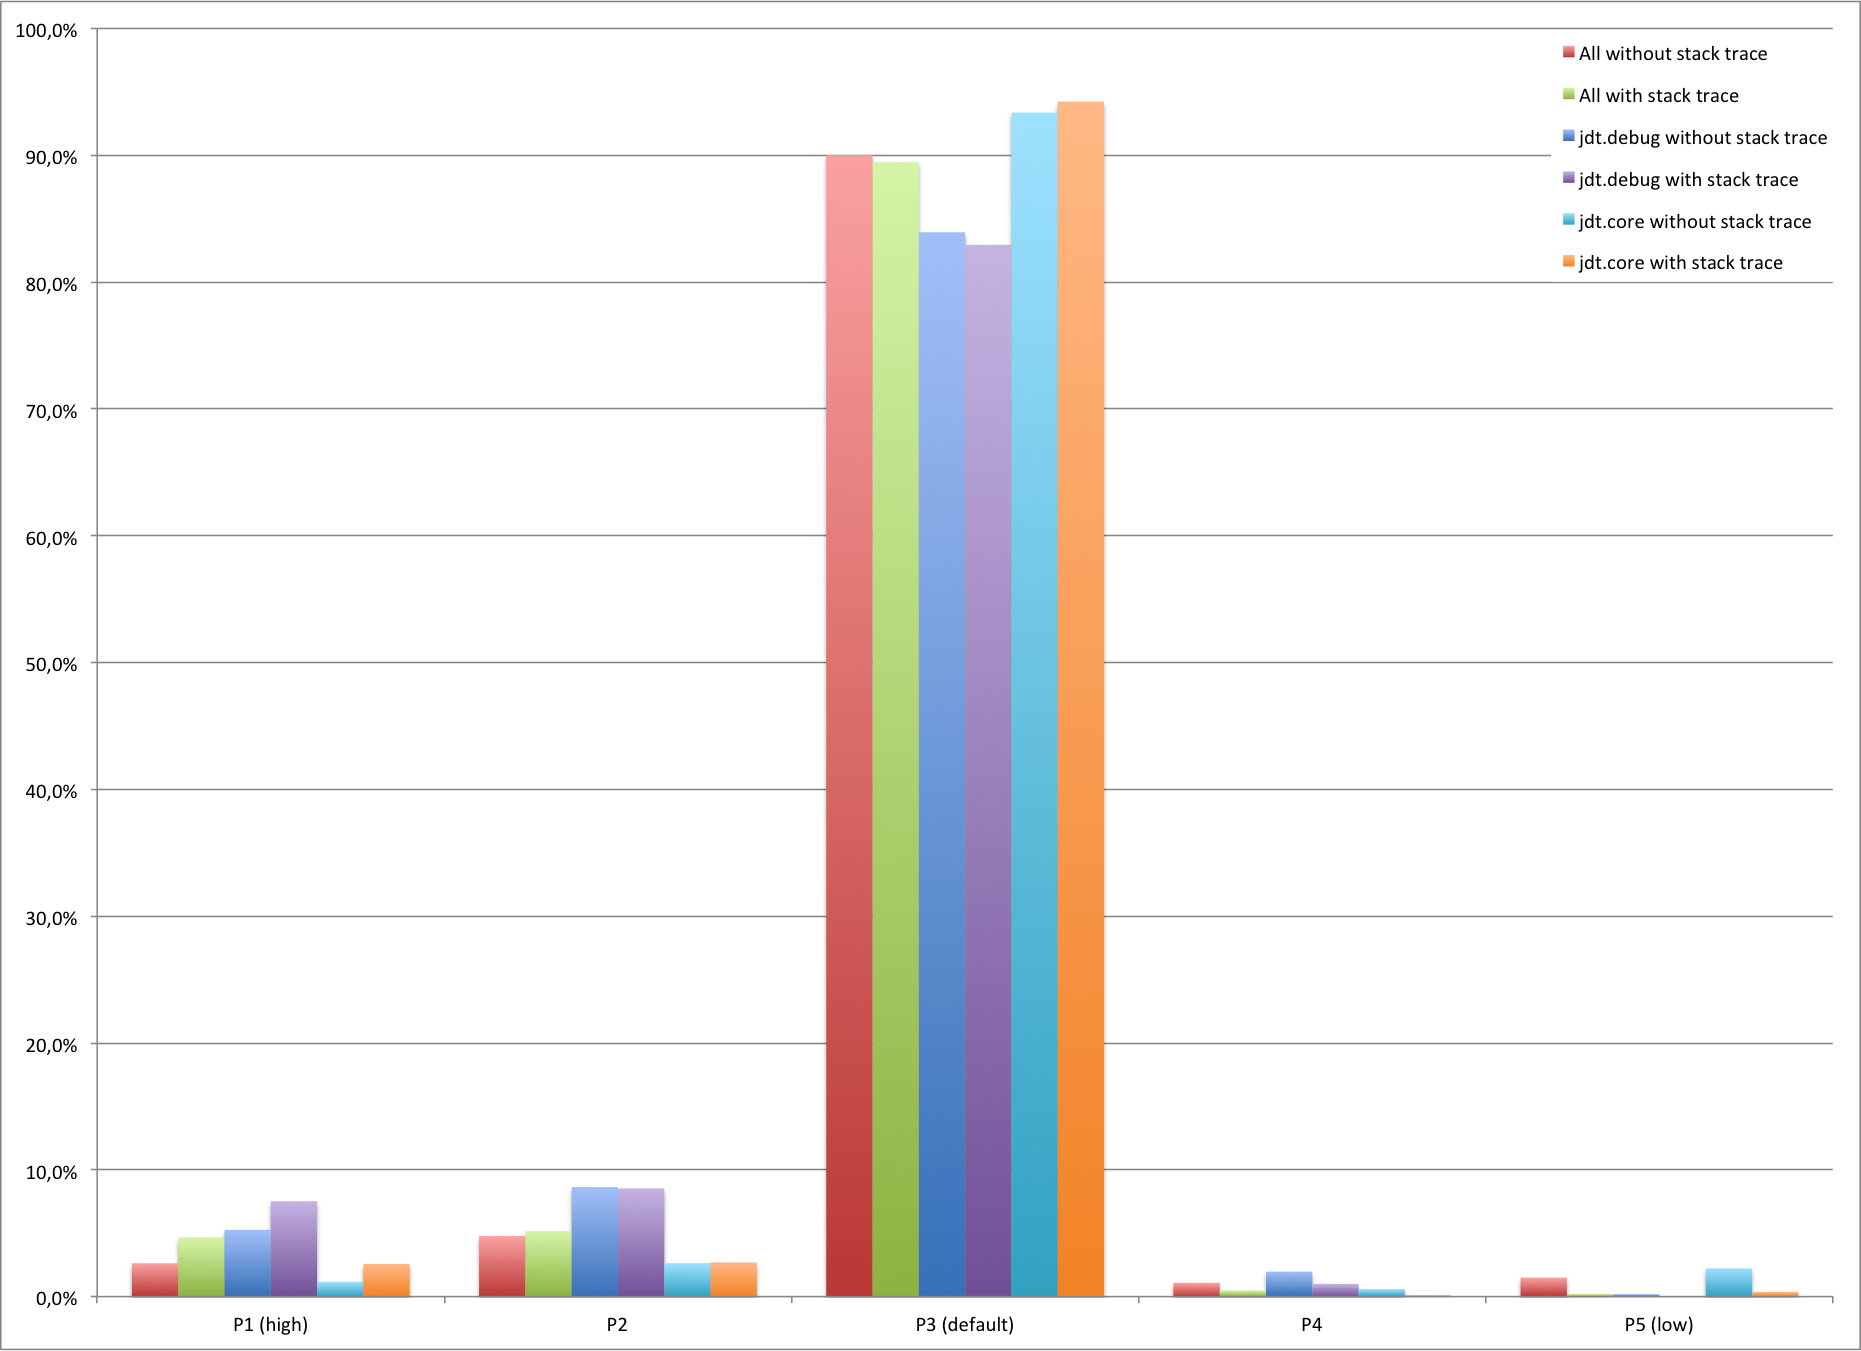
\includegraphics[width=1\textwidth]{img/priority.png}
	\caption{Distribution of priority for issues with and without stack traces.}
	\label{fig:priority}
\end{figure}
% subsection priority (end)

\section{Severity} % (fold)
\label{sec:severity}
Next to priority, every bug report is also assigned a severity. The severity of a bug report is expressed on a 7-level scale: 
\begin{inparaenum}[(1)]
\item blocker,
\item critical,
\item major,
\item normal,
\item minor, and
\item trivial. Also, a severity
\item enhancement is present.
\end{inparaenum}
The latter severity is discarded in this research, since it is used for enhancement requests, and not for bug reports.

Table~\ref{tab:severity} shows the distribution of the bug reports of the two projects, including a breakdown into bugs reports with and without a stack trace. The same data is also visualised in Figure~\ref{fig:severity}, showing a boxplot with and without outliers. Again, many outliers can be spotted in subfigure a.

Overall, 80\% of all bug reports have the default severity `normal'. Around one in ten bug reports is considered to have a major impact. Just like with the priority attribute, an overall shift towards the higher severity can be seen in the bar plot.  

When all bug reports are split into two groups, with and without stack traces, it seems that bug reports with a stack trace tend to have a higher severity. Whether or not there is a relation between the severity of a bug report and the presence of a stack trace is investigated in Section~\ref{sec:analysis_of_priority_and_severity_related_to_the_presence_of_a_stack_trace}.

\begin{table}[!ht]\footnotesize
	\centering
	\begin{tabular}{lrrrrrr}
		\toprule
		& jdt.debug && jdt.core && overall & \\
		\midrule
		All bug reports & 6,492 && 12,221 && 18,713 & \\
		\midrule
		Blocker & 70 & 1.1\% & 159 & 1.3\% & 229 & 1.2\%\\
		Critical & 267 & 4.1\% & 392 & 3.2\% & 659 & 3.5\%\\
		Major & 493 & 7.6\% & 1,170 & 9.6\% & 1,663 & 8.9\%\\
		Normal & 5,285 & 81.4\% & 9,781 & 80.0\% & 15,066 & 80.5\%\\
		Minor & 267 & 4.1\% & 579 & 4.7\% & 846 & 4.5\%\\
		Trivial & 110 & 1.7\% & 140 & 1.1\% & 250 & 1.3\%\\
		\\
		\midrule
		Bug reports without stack trace & 5,904 && 11,416 && 17,320 \\
		\midrule
		Blocker & 61 & 1.0\% & 136 & 1.2\% & 197 & 1.1\%\\
		Critical & 239 & 4.0\% & 352 & 3.1\% & 591 & 3.4\%\\
		Major & 433 & 7.3\% & 1,049 & 9.2\% & 1,482 & 8.6\%\\
		Normal & 4,809 & 81.5\% & 9,176 & 80.4\% & 13,985 & 80.7\%\\
		Minor & 256 & 4.3\% & 563 & 4.9\% & 819 & 4.7\%\\
		Trivial & 106 & 1.8\% & 140 & 1.2\% & 246 & 1.4\%\\
		\\
		\midrule
		Bug reports with stack trace & 587 && 805 && 1,392 \\
		\midrule
		Blocker & 9 & 1.5\% & 23 & 2.9\% & 32 & 2.3\%\\
		Critical & 28 & 4.8\% & 40 & 5.0\% & 68 & 4.9\%\\
		Major & 59 & 10.1\% & 121 & 15.0\% & 180 & 12.9\%\\
		Normal & 477 & 81.3\% & 604 & 75.0\% & 1,081 & 77.7\%\\
		Minor & 11 & 1.9\% & 17 & 2.1\% & 28 & 2.0\%\\
		Trivial & 3 & 0.5\% & 0 & 0.0\% & 3 & 0.2\%\\
		\bottomrule
	\end{tabular} 
	\caption{Statistics for severity.}
	\label{tab:severity}
\end{table}

\begin{figure}[!ht]
	\centering
		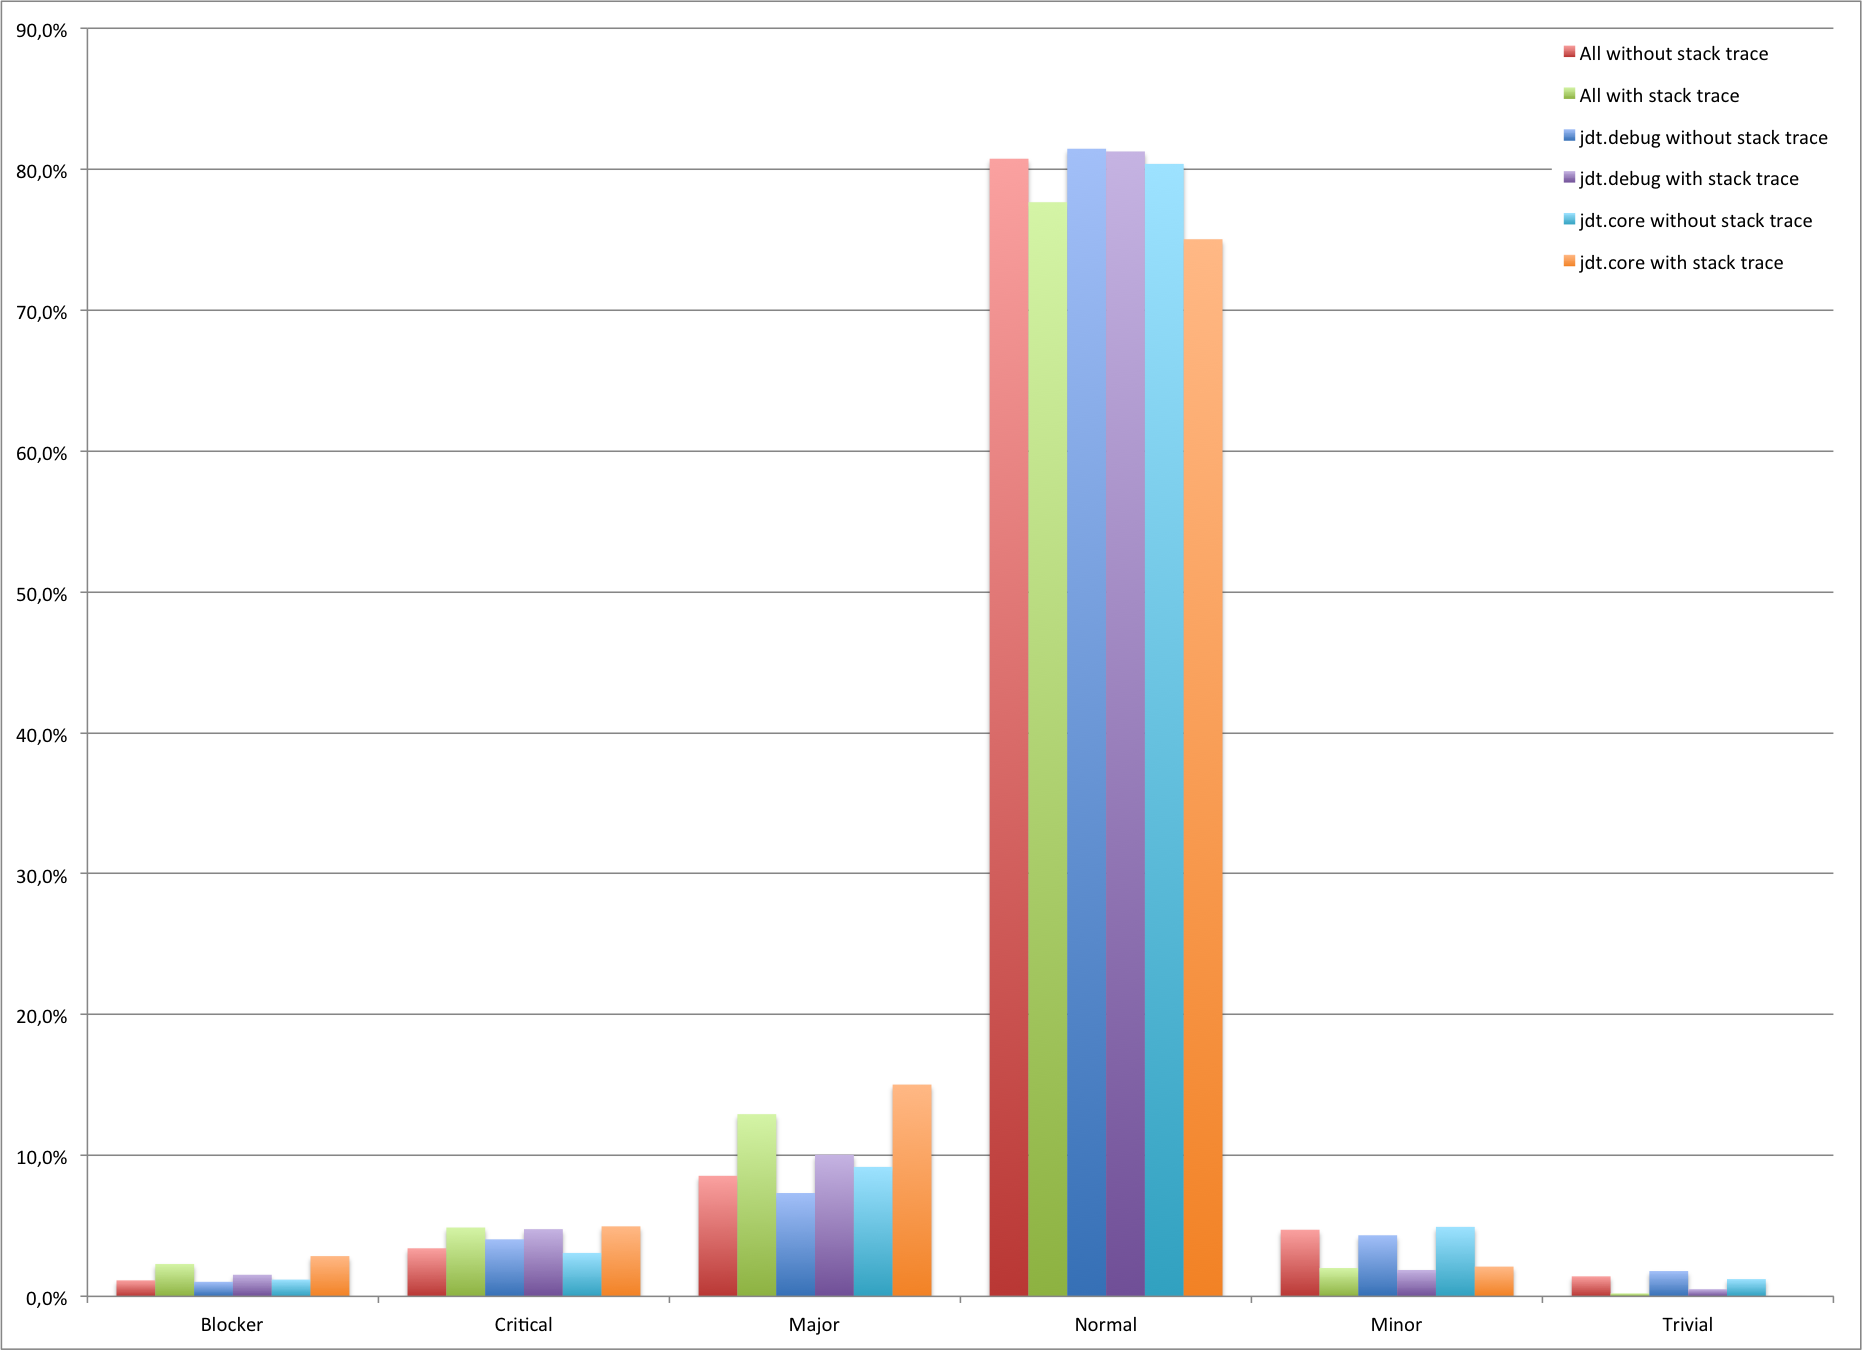
\includegraphics[width=1\textwidth]{img/severity.png}
	\caption{Distribution of severity for issues with and without stack traces}
	\label{fig:severity}
\end{figure}
% subsection severity (end)

\section{Time-to-fix} % (fold)
\label{sec:time_to_fix}
Figure~\ref{fig:ttf-stats} shows the time-to-fix distribution for bug reports for \texttt{jdt.debug}. Since only bugs that meet a specific search query are imported for \texttt{jdt.core}, data for this project is not shown. Some statistics are shown in Table~\ref{tab:ttf-stats}. For jdt.debug, around 30\% of all fixed bug reports have been fixed within a day. In this research, these bugs are discarded, since they probably are only created for administrative reasons. As can be seen, at least one bug is still open after over 8.5 years. The mean fix time is around three months, with a median fix time of 2.5 weeks. 

\begin{table}[!ht]\footnotesize
	\centering
	\begin{tabular}{lrrrrrr}
		\toprule
		project & min & max & mean & median & std \\
		\midrule
		jdt.debug & 1 & 3,137 & 95 & 18 & 225 \\
		\bottomrule
	\end{tabular} 
	\caption{Time-to-fix statistics for jdt.debug (in days).}
	\label{tab:ttf-stats}
\end{table}

\begin{figure}
        \begin{subfigure}[b]{0.48\textwidth}
                \centering
                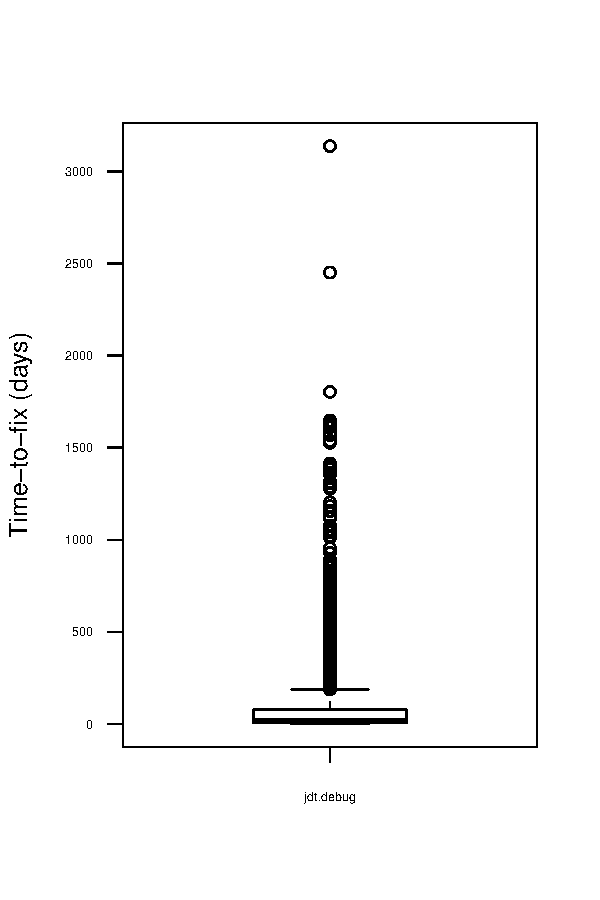
\includegraphics[width=\textwidth]{img/ttf.pdf}
                \caption{Time-to-fix (in days)}
        \end{subfigure}%
        ~ %add desired spacing between images, e. g. ~, \quad, \qquad etc. 
          %(or a blank line to force the subfigure onto a new line)
        \begin{subfigure}[b]{0.48\textwidth}
                \centering
                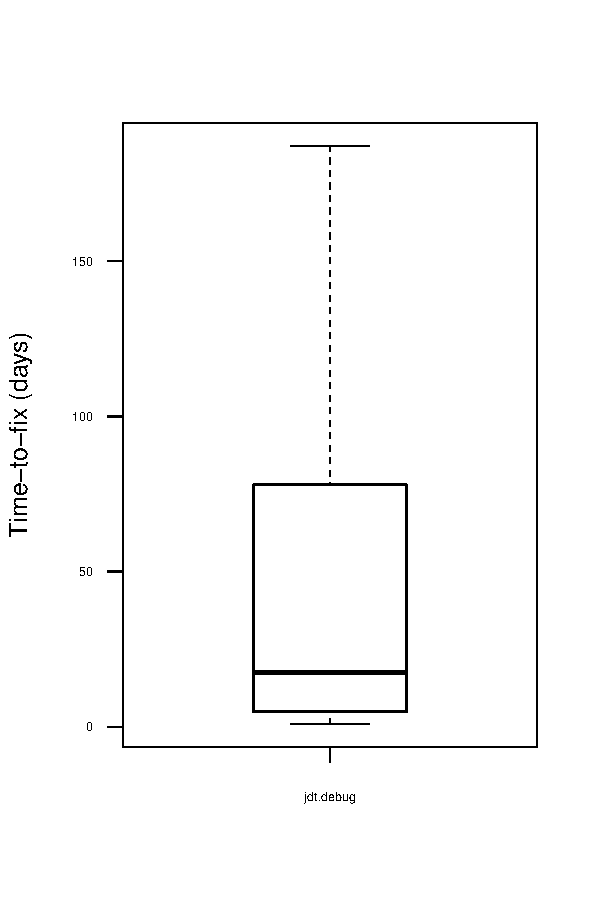
\includegraphics[width=\textwidth]{img/ttf-zoomed.pdf}
                \caption{Time-to-fix (without outliers, in days)}
        \end{subfigure}
		\caption{Time-to-fix statistics for jdt.debug}
		\label{fig:ttf-stats}
\end{figure}

% subsection time_to_fix (end)

\section{Class size} % (fold)
\label{sec:class_size}
Table~\ref{tab:class-stats} shows descriptive statistics for class size. For these measurements, the complete file history of each project is taken into account. For each class, the latest revision of that file is used for the lines of code measurement. The class size is also visualised in Figure~\ref{fig:class-stats}. Project's \texttt{jdt.debug} history contained 714 classes, \texttt{jdt.core} contained 1,715 classes. Please note these numbers include \emph{all} classes from the project history, also classes that are not present anymore in the latest revision of the project.

\begin{table}[!ht]\footnotesize
	\centering
	\begin{tabular}{lrrrrrr}
		\toprule
		project & N & min & max & mean & median & std \\
		\midrule
		jdt.debug & 714 & 2 & 2,628 & 73 & 15 & 198 \\
		jdt.core & 1,715 & 1 & 10,928 & 201 & 58 & 581 \\
		\bottomrule
	\end{tabular} 
	\caption{Class size statistics for each project (full history). N is the number of classes.}
	\label{tab:class-stats}
\end{table}
 
\begin{figure}
        \begin{subfigure}[b]{0.48\textwidth}
                \centering
                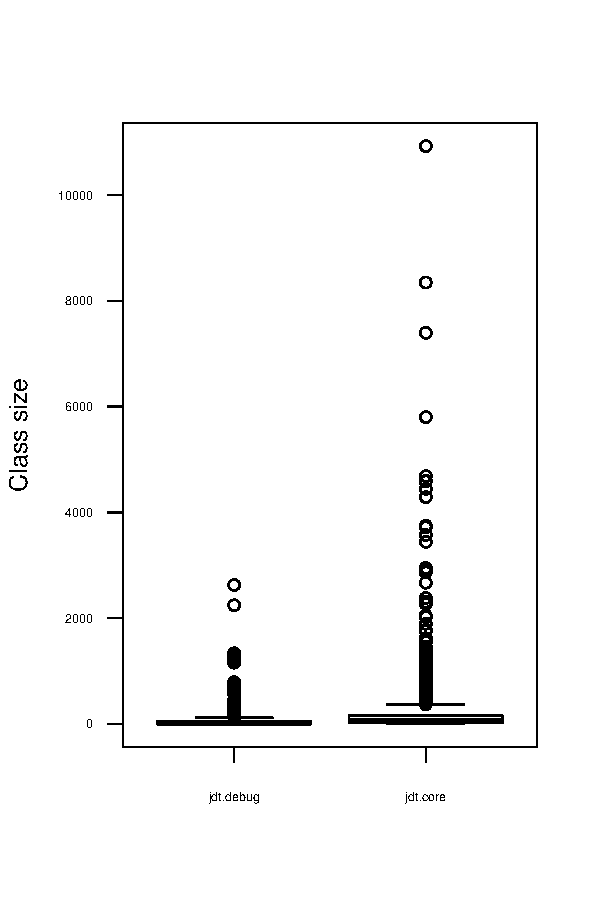
\includegraphics[width=\textwidth]{img/class-size-boxplot.pdf}
                \caption{Class size}
        \end{subfigure}%
        ~ %add desired spacing between images, e. g. ~, \quad, \qquad etc. 
          %(or a blank line to force the subfigure onto a new line)
        \begin{subfigure}[b]{0.48\textwidth}
                \centering
                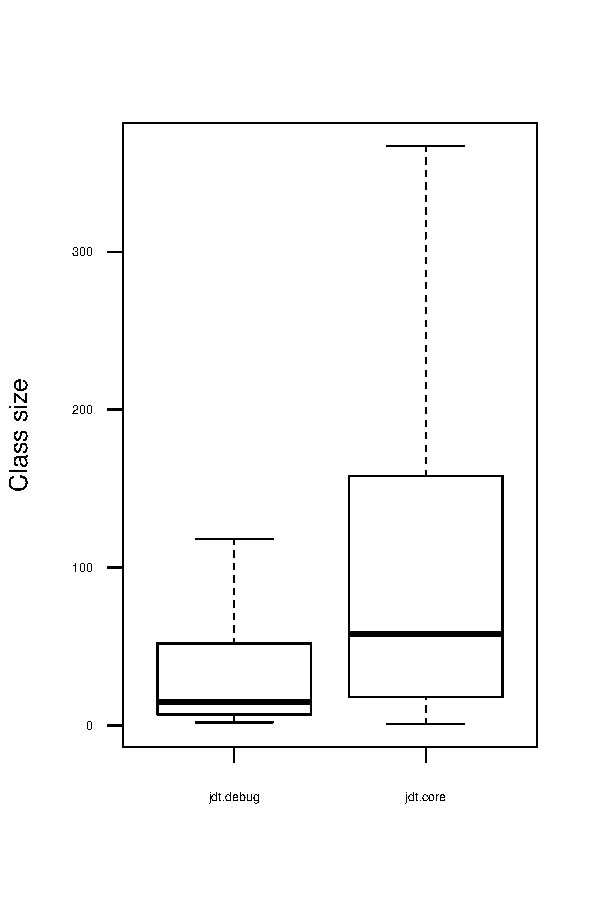
\includegraphics[width=\textwidth]{img/class-size-boxplot-zoomed.pdf}
                \caption{Class size (without outliers)}
        \end{subfigure}
		\caption{Class size statistics for each project (full history)}
		\label{fig:class-stats}
\end{figure}

When looking at the maximum number of lines of code, it can be seen that some classes have a very high number of lines of code. Although this looks quite odd, several source files in \texttt{jdt.debug} and \texttt{jdt.core} do indeed have such a high amount of lines of code ($> 30,000$, comments and white lines included\footnote{In Table~\ref{tab:class-stats}, white lines and comments are excluded, resulting in a far lower number.}). Also, there is quite a difference in mean (4.5 months) and median (almost 1.5 month) time-to-fix between \texttt{jdt.debug} and \texttt{jdt.core}. The box plot also shows this difference, where in subfigure b, the median value shows a particular shift, and the box plot for \texttt{jdt.core} spans a bigger range.
% subsection class_size (end)

\section{Package size} % (fold)
\label{sec:descr:package_size}
Table~\ref{tab:package-stats} shows the descriptive statistics for the three definitions of package size (see Section~\ref{sub:da:analysis_of_priority_and_severity_related_to_package_size}):

\begin{enumerate*}
	\item number of classes (NOC)
	\item total lines of code of associated classes (SUMLOC)
	\item (arithmetic) mean of lines of code of associated classes (AVGLOC)
\end{enumerate*}

The visualisations of these six measurements using a box plot are shown in Figures \ref{fig:package-stats} and \ref{fig:package-stats-zoomed}, where outliers are discarded from the latter box plot. For each underlying class, the latest revision is used for the lines of code measurement. Project \texttt{jdt.debug} contained 29 packages, \texttt{jdt.core} contained 65 packages. Please note these numbers include \emph{all} packages and classes from the project history, also packages and classes that are not present anymore in the latest revision of the project.

\begin{table}[!ht]\footnotesize
	\centering
	\begin{tabular}{lrrrrr}
		\toprule
		project & min & max & mean & median & std \\
		\midrule
		NOC\\
		\midrule
		jdt.debug & 4 & 178 & 49 & 32 & 47 \\
		jdt.core & 2 & 408 & 53 & 30 & 78 \\
		\midrule
		SUMLOC\\
		\midrule
		jdt.debug & 21 & 9,613 & 1,803 & 673 & 2,697 \\
		jdt.core & 2 & 36,798 & 5,313 & 2,099 & 8,024 \\
		\midrule
		AVGLOC\\
		\midrule
		jdt.debug & 1 & 129 & 37 & 18 & 40 \\
		jdt.core & 1 & 595 & 108 & 74 & 116 \\
		\bottomrule
	\end{tabular} 
	\caption{Package statistics for each project. Packages with no classes are discarded.}
	\label{tab:package-stats}
\end{table}
 
\begin{figure}
        \begin{subfigure}[b]{0.48\textwidth}
                \centering
                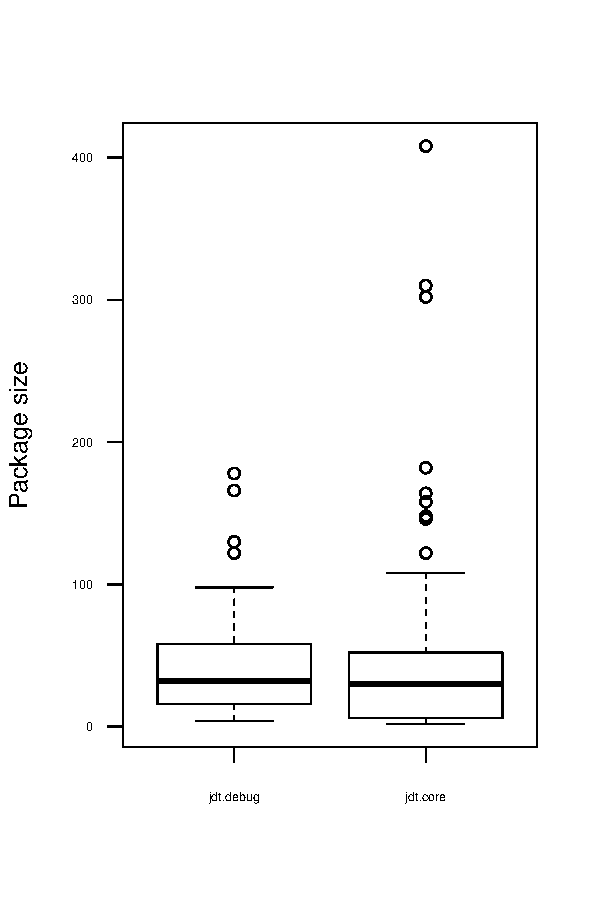
\includegraphics[width=\textwidth]{img/package-size-noc.pdf}
                \caption{NOC}
        \end{subfigure}%
        ~ %add desired spacing between images, e. g. ~, \quad, \qquad etc. 
          %(or a blank line to force the subfigure onto a new line)
        \begin{subfigure}[b]{0.48\textwidth}
                \centering
                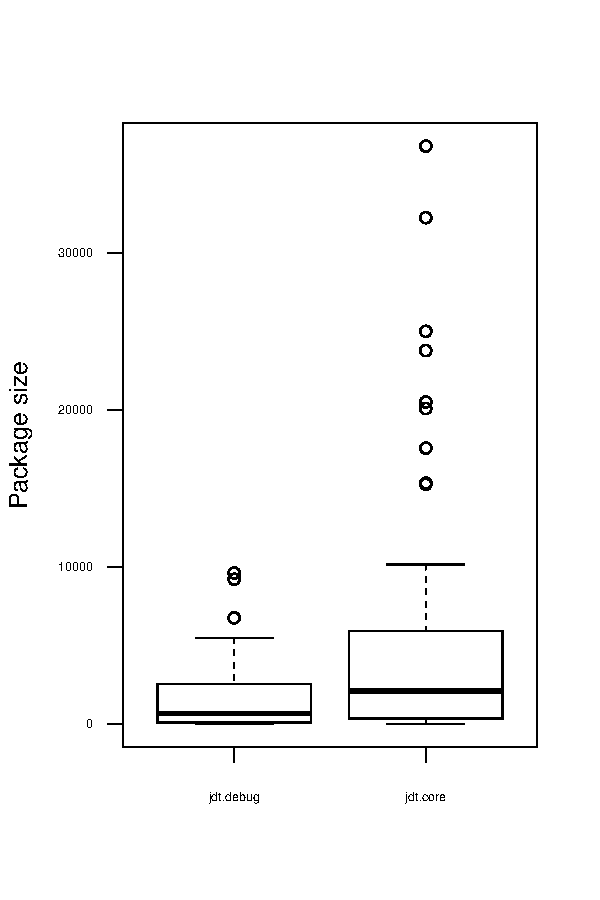
\includegraphics[width=\textwidth]{img/package-size-sumloc.pdf}
                \caption{SUMLOC}
        \end{subfigure}

        \begin{subfigure}[b]{0.48\textwidth}
                \centering
                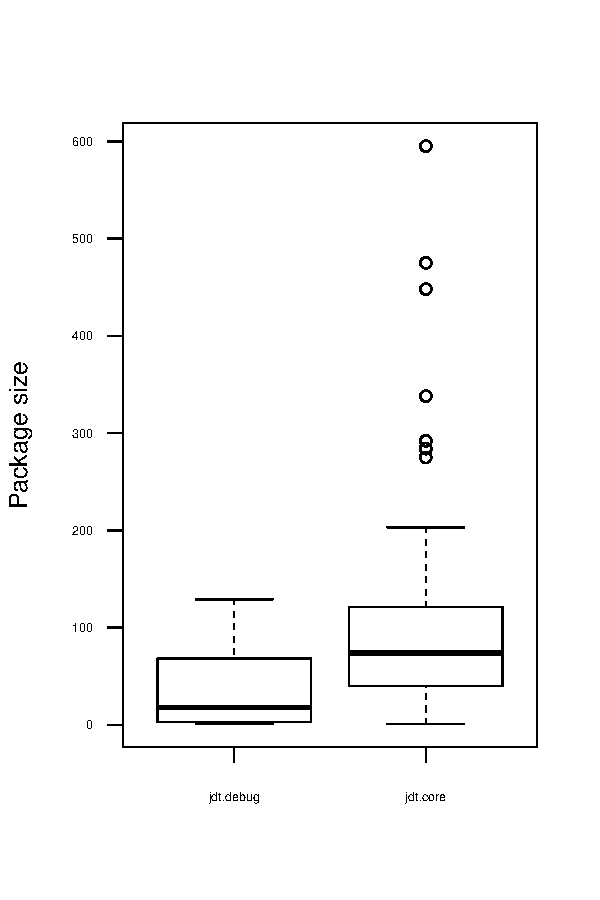
\includegraphics[width=\textwidth]{img/package-size-avgloc.pdf}
                \caption{AVGLOC}
        \end{subfigure}
		\caption{Package size statistics (full history). Packages with no classes are discarded.}
		\label{fig:package-stats}
\end{figure}

\begin{figure}
        \begin{subfigure}[b]{0.48\textwidth}
                \centering
                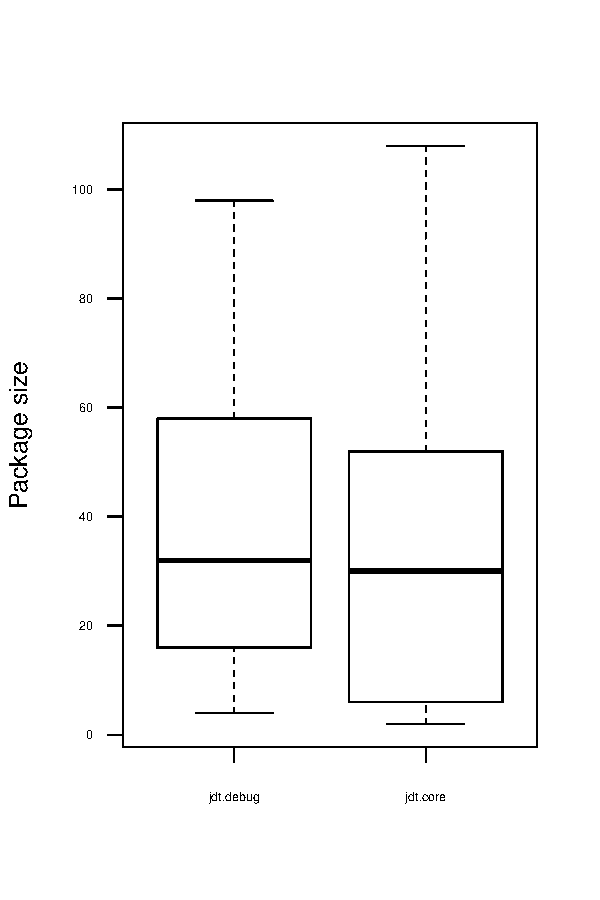
\includegraphics[width=\textwidth]{img/package-size-noc-zoomed.pdf}
                \caption{NOC}
        \end{subfigure}%
        ~ %add desired spacing between images, e. g. ~, \quad, \qquad etc. 
          %(or a blank line to force the subfigure onto a new line)
        \begin{subfigure}[b]{0.48\textwidth}
                \centering
                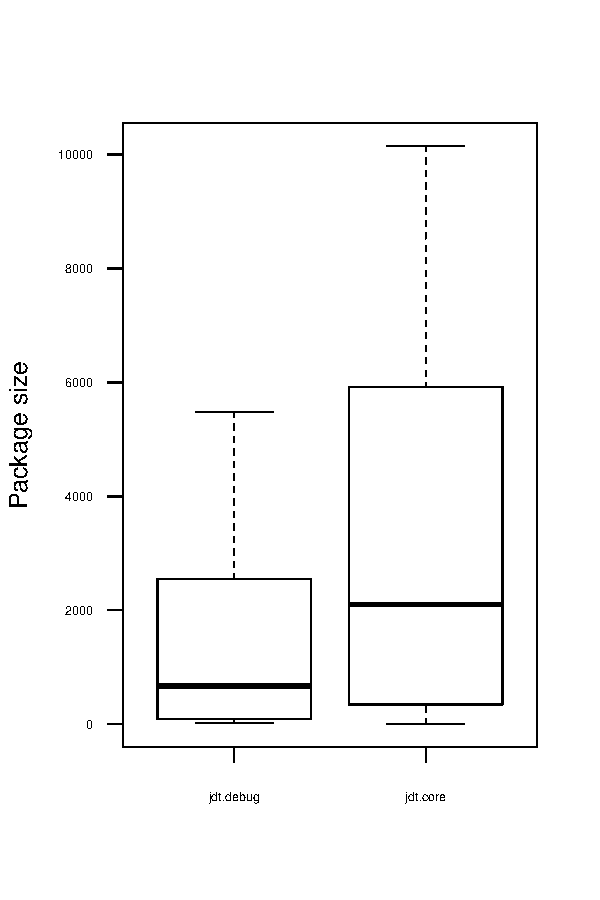
\includegraphics[width=\textwidth]{img/package-size-sumloc-zoomed.pdf}
                \caption{SUMLOC}
        \end{subfigure}

        \begin{subfigure}[b]{0.48\textwidth}
                \centering
                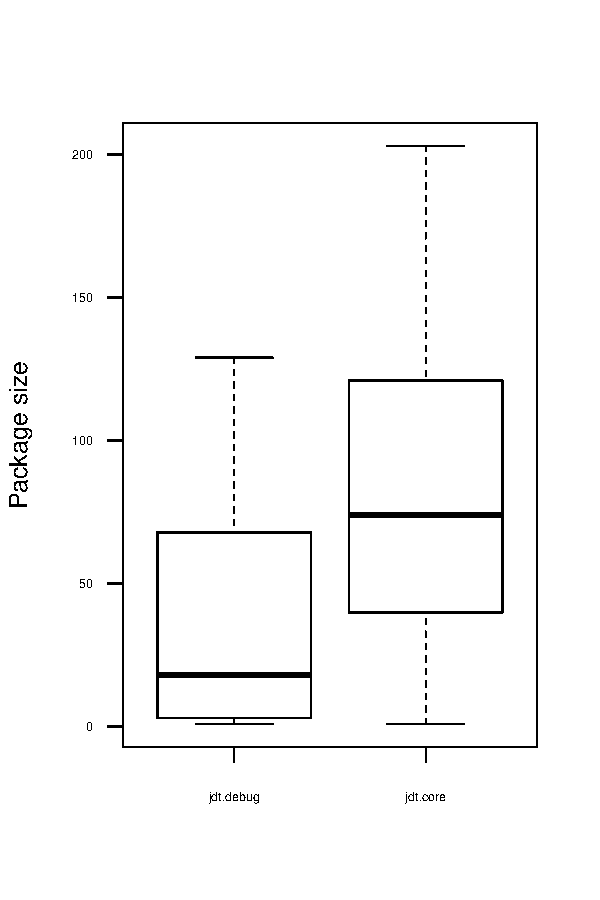
\includegraphics[width=\textwidth]{img/package-size-avgloc-zoomed.pdf}
                \caption{AVGLOC}
        \end{subfigure}
		\caption{Package size statistics (full history), without outliers. Packages with no classes are discarded.}
		\label{fig:package-stats-zoomed}
\end{figure}

A package in \texttt{jdt.debug} on average consists of 20 classes. This number increases to 26 for \texttt{jdt.core}. Some packages do not contain classes at all (they only contain sub-packages) and are discarded from the data set.

When looking at the total lines of code of the associated classes for a package (SUMLOC), it can be seen that some packages have a very high number of total lines of code. This is again due to the fact that several source files have a high amount of lines of code. The AVGLOC metric averages the total number of lines of all classes in a package over the number of classes in a package. This way, the influence of the number of classes in a package in cancelled out.

As can be seen in Figure~\ref{fig:package-stats-zoomed}, each package has a specific `signature' for each metric. This supports the theory that each software project should be treated in isolation, i.e., data sets should not be combined into one large data set.
% subsection package_size (end)

% chapter descriptive_statistics (end)
%!TEX root = thesis.tex

\chapter{Results: Priority and Severity} % (fold)
\label{cha:results_priority_and_severity}

In this chapter, the first research question and the accompanying hypothesis are investigated, as defined in Section~\ref{sec:research_questions}:

\vspace{\baselineskip}
\questiona{}
\vspace{\baselineskip}

\noindent
In order to answer this question, certain relationships need to be present in the data. To research if these relationships are present, the following hypotheses are stated:

\vspace{\baselineskip}
\hypaa{}

\vspace{\baselineskip}
\hypab{}

\vspace{\baselineskip}
\hypac{}

\vspace{\baselineskip}
\hypad{}

\vspace{\baselineskip}
\hypae{}

\vspace{\baselineskip}
\hypaf{}

\vspace{\baselineskip}

\section{Overview} % (fold)
All investigations in this chapter are split into three parts: 
\begin{inparaenum}[(1)]
\item \textbf{results}, describing the direct results of the study and showing some descriptive statistics,
\item \textbf{analysis}, analysing the results of the study, and
\item \textbf{conclusions}, which evaluates the hypotheses.
\end{inparaenum}

In Section~\ref{sec:analysis_of_priority_and_severity_related_to_the_presence_of_a_stack_trace}, a possible relation between priority (and severity) of bug reports with the presence of one or more stack traces is investigated. Section~\ref{sec:analysis_of_priority_and_severity_related_to_package_size} investigates if the priority and severity of a bug report tend to be higher if the corresponding packages for the stack trace(s) in the bug report have a larger size. The same investigation is performed on class level in Section~\ref{sec:analysis_of_priority_and_severity_related_to_lines_of_code}.

Finally, all results found in the previous mentioned sections are summarised in Section~\ref{sec:priosev-summary_of_results}.
% section overview (end)

\section{Analysis of priority and severity related to the presence of a stack trace} % (fold)
\label{sec:analysis_of_priority_and_severity_related_to_the_presence_of_a_stack_trace}
When a stack trace is present, a bug triager might be able to identify the location of a bug in source code more easily. This way, it might be also easier to assign a representative priority and severity to the bug report (i.e., less bugs with default priority and severity).

As can be seen in Tables \ref{tab:priority} and \ref{tab:severity}, some small differences exists between the presence of a stack trace versus priority, as well as for the presence of a stack trace versus severity. For example, around 2.5\% more bug reports with priority higher than normal are counted when a stack trace is present. Also, the number of bug reports with severity higher than normal shows a 7.0\% increase.

In this section, we investigate if there is a relation between priority versus presence of a stack trace. The same investigation is performed for severity. In short, the following two hypotheses of research question R1 are discussed: 

\vspace{\baselineskip}
\hypaa{}

\vspace{\baselineskip}
\hypab{}
\vspace{\baselineskip}

\subsection{Results} % (fold)
The count results for priority can be found in Table~\ref{tab:prio-counts}. It shows, for both the two projects as well for the overall situation, the number of bug reports for each priority. A distinction is made between bug reports with a stack trace present, and bug reports without a stack trace in the comments. In Table~\ref{tab:sev-counts}, the same data is presented for the severity.

\begin{table}[!ht]\footnotesize
	\centering
	\begin{tabular}{lrrrrrrr}
		\toprule		
		 & \texttt{jdt.debug} &  & \texttt{jdt.core} &  & overall & \\
		priority & w/o trace & w/ trace & w/o trace & w/ trace & w/o trace & w/ trace\\
		\midrule
		P1 (high) & 380 & 45 & 153 & 21 & 533 & 66\\
		P2 & 623 & 51 & 344 & 22 & 967 & 73\\
		P3 (default) & 6,056 & 496 & 12,190 & 769 & 18,246 & 1,265\\
		P4 & 142 & 6 & 78 & 1 & 220 & 7\\
		P5 (low) & 14 & 0 & 290 & 3 & 304 & 3\\
		\bottomrule
	\end{tabular} 
	\caption{Number of bug reports for each priority.}
	\label{tab:prio-counts}
\end{table}

\begin{table}[!ht]\footnotesize
	\centering
	\begin{tabular}{lrrrrrrr}
		\toprule		
		 & \texttt{jdt.debug} &  & \texttt{jdt.core} &  & overall & \\
		severity & w/o trace & w/ trace & w/o trace & w/ trace & w/o trace & w/ trace\\
		\midrule
		Blocker & 61 & 9 & 136 & 23 & 197 & 32\\
		Critical & 239 & 28 & 352 & 40 & 591 & 68\\
		Major & 433 & 59 & 1,049 & 121 & 1,482 & 180\\
		Normal & 4,809 & 477 & 9,176 & 604 & 13,985 & 1,081\\
		Minor & 256 & 11 & 563 & 17 & 819 & 28\\
		Trivial & 106 & 3 & 140 & 0 & 246 & 3\\
		\bottomrule
	\end{tabular} 
	\caption{Number of bug reports for each severity.}
	\label{tab:sev-counts}
\end{table}
% subsection results (end)

\subsection{Analysis} % (fold)
To test whether there is an association between priority and presence of a stack trace (and between severity and presence of a stack trace), a statistical test of independence is performed. The null hypothesis of such a test states `there is no association between two variables', where the alternative hypothesis states `the two variables are associated'. Since the data under test is categorical data (i.e., count data), a chi-squared test is used (see Section~\ref{sub:chi_squared_test}). In total, a number of six chi-squared tests are executed; tests for \texttt{jdt.debug}, \texttt{jdt.core} and the overall situation, for both priority and severity. 

The validity of a chi-squared test depends on the sample size of the whole dataset and the \emph{expected} theoretical cell counts. For all six tests, the chi-squared approximation is adequate.

The results of the six association tests can be found in Table~\ref{tab:chi2}.

\begin{table}[!ht]\footnotesize
	\centering
	\begin{tabular}{lrrl}
		\toprule		
		association & $\chi^2$ & $p$ & \\
		\midrule
		priority -- \texttt{jdt.debug} & $\chi^2(4, N=7,813) = 9.12$ & $0.058$ & \\
		priority -- \texttt{jdt.core} & $\chi^2(4, N=13,871) = 27.63$ & $< 0.001$ & ***\\
		priority -- overall & $\chi^2(4, N=21,684) = 40.22$ & $< 0.001$ & ***\\
		\midrule
		severity -- \texttt{jdt.debug} & $\chi^2(5, N=6,491) = 20.23$ & $0.001$ & *** \\
		severity -- \texttt{jdt.core} & $\chi^2(5, N=12,221) = 76.34$ & $< 0.001$ & *** \\
		severity -- overall & $\chi^2(5, N=18,712) = 86.49$ & $< 0.001$ & ***\\
		\bottomrule
	\end{tabular} 
	\caption{Chi-squared test results. Format: $\chi^2(df, N=n)$, with $df$ the degree of freedom, and $n$ the number of counts.}
	\label{tab:chi2}
\end{table}

\subsubsection{Priority} % (fold)
Overall, 90\% of all bug reports is assigned the default priority P3. For each separate data set (\texttt{jdt.debug} and \texttt{jdt.core}), the default priority P3 is respectively 84\% and 93\%. For \texttt{jdt.debug}, around 14\% of all bugs get assigned a higher than normal priority, compared to only 4\% for \texttt{jdt.core}. 

When the overall data set is split into two groups --- bug reports with and without one or more stack traces --- some differences can be spotted. The percentage of bugs that get assigned priority P3 deceases with 1.0\% for \texttt{jdt.debug} and increases with 0.8\% for \texttt{jdt.core}. For \texttt{jdt.debug}, 13.9\% of all bug reports without a stack trace get assigned a higher than normal priority, compared to 16.0\% for bug reports that include a stack trace, resulting in an increase of 2.1\%. For \texttt{jdt.core}, an increase of 1.5\% is shown, going from 3.8\% for bug reports without a stack trace, to 5.3\% for bug reports that include a stack trace. 

As expected, the opposite result is visible in the number of bug reports with a lower than normal priority. For \texttt{jdt.debug}, a decrease of 1.2\% is shown, and for \texttt{jdt.core} a decrease of 2.3\%.

Despite these numbers, the chi-squared test does not show a significant result for \texttt{jdt.debug}, accepting the hypothesis that there is no association between priority and the presence of a stack trace. This can be explained by looking at the contribution of each association to the overall chi-squared statistic\footnote{see Section~\ref{sub:chi_squared_test}}. Only the particular association between \texttt{jdt.debug} and P1 shows a significant difference.

For \texttt{jdt.core}, the chi-squared test does show a significant result, rejecting the null hypothesis and giving evidence that there is an association between the variables (but not \emph{which} association). When looking at the contribution of each association to the overall chi-squared statistic, P1 and P5 show a significant difference, which can be attributed to the increase of 1.4\% for P1 and decease of 1.8\% for P5.

For the combined data set, a significant result for the chi-square test is shown. Most attribution for this is, again, for the increase of P1 and decrease of P5.
% subsubsection priority (end)

\subsubsection{Severity} % (fold)
Overall, 80\% of all bug reports is assigned the default severity `normal' and around 9\% is considered a `major' bug report. Compared to the priority attribute, around 10\% less bug reports is assigned the default severity. Overall, 14\% of all bug reports get assigned a higher than normal severity, and around 6\% a less than normal severity. These numbers are similar for the \texttt{jdt.debug} and \texttt{jdt.core} data sets.

When the overall data set is split into two groups --- bug reports with and without one or more stack traces --- some differences can again be spotted. The percentage of bugs that get assigned severity `normal' deceases with 5.4\% for \texttt{jdt.core}, but does not change much for \texttt{jdt.debug}. For \texttt{jdt.debug}, 12.3\% of all bug reports without a stack trace get assigned a higher that normal severity, compared to 16.4\% for bug reports that include a stack trace. This results in an increase of 4.1\%. For \texttt{jdt.core}, an increase of 9.4\% is shown, going from 13.5\% for bug reports without a stack trace, to 22.9\% for bug reports that include a stack trace. 

This increase in higher severity bug reports that include a stack trace is also reflected in the number of bug reports with a lower than normal severity. For \texttt{jdt.debug}, a decrease of 3.7\% is shown, for \texttt{jdt.core} a decrease of 4.0\%.

The chi-squared tests show a highly significant result for \texttt{jdt.debug}, \texttt{jdt.core} and the overall data set, rejecting the hypothesis that there is no association between severity and the presence of a stack trace. This can be explained by looking at the contribution of each association to the overall chi-squared statistic. The attribution of each value for a bug report with a stack trace is significant, except for the `normal' severities and `blocker' and `critical' severities in the case of \texttt{jdt.debug}.
% subsubsection severity (end)
% subsection analysis (end)

\subsection{Conclusions} % (fold)
As can be seen in Tables \ref{tab:priority} and \ref{tab:severity} and their graphical representations in Figure \ref{fig:priority} and \ref{fig:severity}, some differences can be noted between bug reports with and without a stack trace. The results of the chi-square test in Table~\ref{tab:chi2} also shows some significant results.

In \cite{Bettenburg2007} and \cite{Zimmermann2010}, it is shown that the presence of a stack trace is a sign of quality of a bug report. High quality bug reports are likely to get more attention from developers and triagers, which might also be why they get assigned a more representative priority and severity, instead of the default value.

\subsubsection{Priority} 
For \texttt{jdt.debug}, no evidence for an association between priority and presence of a stack trace is found, but the number of high priority bug reports does increase and the number of low priority bug reports does decrease when a stack trace is present. On the other hand, for \texttt{jdt.core} and the overall data set, evidence is found for an association between priority and the presence of a stack trace. When investigating the contribution of each association\footnote{Please refer to Section~\ref{sub:chi_squared_test}} to the overall chi-squared statistic and the bar charts, some evidence is found that bug reports with a stack trace are more common assigned priority P1 (2.6\% versus 4.6\% for the overall situation). Also, the number of low priority bugs decreases when a stack trace is present (2.6\% versus 0.7\% for the overall situation). This gives enough evidence to at least partially accept hypothesis High:

\vspace{\baselineskip}
\hypaa{}
\vspace{\baselineskip}

\noindent
Schr\"{o}ter \emph{et al.} \cite{Schroter2010} showed that stack traces are valuable pointers to points of interest in the source code. We also showed that stack traces can be used as pointers to other bug reports. This way, it might be easier for a triager to assess a better priority for the bug report, since the possible costs for a fix might be easier to determine (by inspecting source code and related bugs).

\subsubsection{Severity}
For all data sets, evidence is found for an association between severity and the presence of a stack trace. When investigating the contribution of each association to the overall chi-squared statistic and the bar charts, the number of bug reports with a higher than normal severity increases when a stack trace is present (13.1\% versus 20.1\% for the overall situation). Also, the number of bug reports with a lower than normal severity decreases when a stack trace is present (6.1\% versus 2.2\% for the overall situation). This gives enough evidence to accept hypothesis H1.2:

\vspace{\baselineskip}
\hypab{}
\vspace{\baselineskip}

\noindent
In \cite{Schroter2010}, it is showed that in up to 60\% of fixed bug reports, the bug is actually fixed in one of the methods mentioned in a stack trace. This means that when a stack trace is present in the bug report, a triager might be able to perform a better assessment of the severity of a bug by inspecting the source code.
% subsection conclusions (end)

% section analysis_of_priority_and_severity_related_to_the_presence_of_a_stack_trace_in_a_bug_report (end)

\section{Analysis of priority and severity related to package size} % (fold)
\label{sec:analysis_of_priority_and_severity_related_to_package_size}
When one or more stack traces are present in comments of a bug report, it is possible to relate each bug report to one or more source packages. A larger package size might point to a more important subsystem of the software, hence to a higher priority or severity of a bug. In this section, it will be investigated whether there is a relation between the priority (and severity) of a bug report and the size of the related packages references in stack traces in this bug reports.

The \emph{size} of a package is not bound to a single evident definition. Three possible definitions are investigated in this section:

\begin{enumerate*}
	\item number of classes (NOC)
	\item total lines of code of associated classes (SUMLOC)
	\item (arithmetic) mean of lines of code of associated classes (AVGLOC)
\end{enumerate*}

Some descriptive statistics for package size can be found in Section~\ref{sec:descr:package_size}.

\subsection{Results} % (fold)
For each bug report with a stack trace, all associated packages are determined, which in turn have the above mentioned size metrics (when their associated classes can be found in the source code repository). A bug report can have multiple stack traces, and a stack trace can have multiple associated packages. This results in a list of pairs \emph{(report, package)}. It is possible that the same stack trace is mentioned multiple times in a bug report (for example in a quoted message). Also, a package can be mentioned multiple times in a stack trace.

In order to make sure these duplicates do not affect the statistics, only unique pairs \emph{(report, package)} are considered. The pair-counts for all issues under investigation can be seen in Table~\ref{tab:package-tuple-counts}. As can be seen, default values P3 and `normal' are most commonly used.

\begin{table}[!ht]\footnotesize
	\centering
	\begin{tabular}{lrrrrrr}
		\toprule
		 & \texttt{jdt.debug} & \texttt{jdt.core} & overall\\
		\midrule
		P1 & 4 & 5 & 9\\
		P2 & 19 & 10 & 29\\
		P3 & 332 & 1,149 & 1,481\\
		P4 & 5 & 0 & 5\\
		P5 & 0 & 9 & 9\\
		\midrule
		Total & 360 & 1,173 & 1,533\\
		\midrule
		\\
		Blocker & 0 & 57 & 57\\
		Critical & 7 & 56 & 63\\
		Major & 39 & 180 & 219\\
		Normal & 308 & 859 & 1,167\\
		Minor & 0 & 19 & 19\\
		Trivial & 0 & 0 & 0\\
		\midrule
		Total & 354 & 1,171 & 1,525\\
		\bottomrule
	\end{tabular} 
	\caption{Unique \emph{(report, package)} pair-counts.}
	\label{tab:package-tuple-counts}
\end{table}
% subsection results (end)

\subsection{Analysis} % (fold)
In order to investigate whether there is a relation between priority (or severity) and package size, a pairwise comparison of the median values of each data set is performed. For priority, P1 and P2 are compared, P2 and P3, et cetera. For severity, `blocker' and `critical' are compared, `critical' and `major', et cetera.

As can be seen in Table~\ref{tab:package-tuple-counts}, the number of data points for non-default priority is very low, which is consistent with the research performed in \cite{Lamkanfi2010}, who found that most bug reports get assigned the default value for priority and severity. This means it is not possible to thoroughly investigate the hypothesis. However, for severity, a analysis can be made in the case of \texttt{jdt.core}. With this data set, three comparisons can be made (`blocker' versus `critical', `critical' versus `major', `major' versus `normal'). Using these three comparisons, a possible relationship between the two dimensions priority (or severity) and package size can be shown.

The box plots for the data sets for all three size metrics under investigation is depicted in Figure~\ref{fig:packages-box-sevcore}. Some descriptive statistics are shown in Table~\ref{tab:package-sev-stats}. For all minimum and maximum values, a lot of similar numbers can be seen for the lines-of-code metric and number of classes metrics. This is probably due to some specific files that are quite common is stack traces. For NOC, a decrease in median and mean values is seen when the severity becomes higher. The same applies to SUMLOC, but no changes can be spotted for AVGLOC.

\begin{figure}
        \begin{subfigure}[b]{0.5\textwidth}
                \centering
                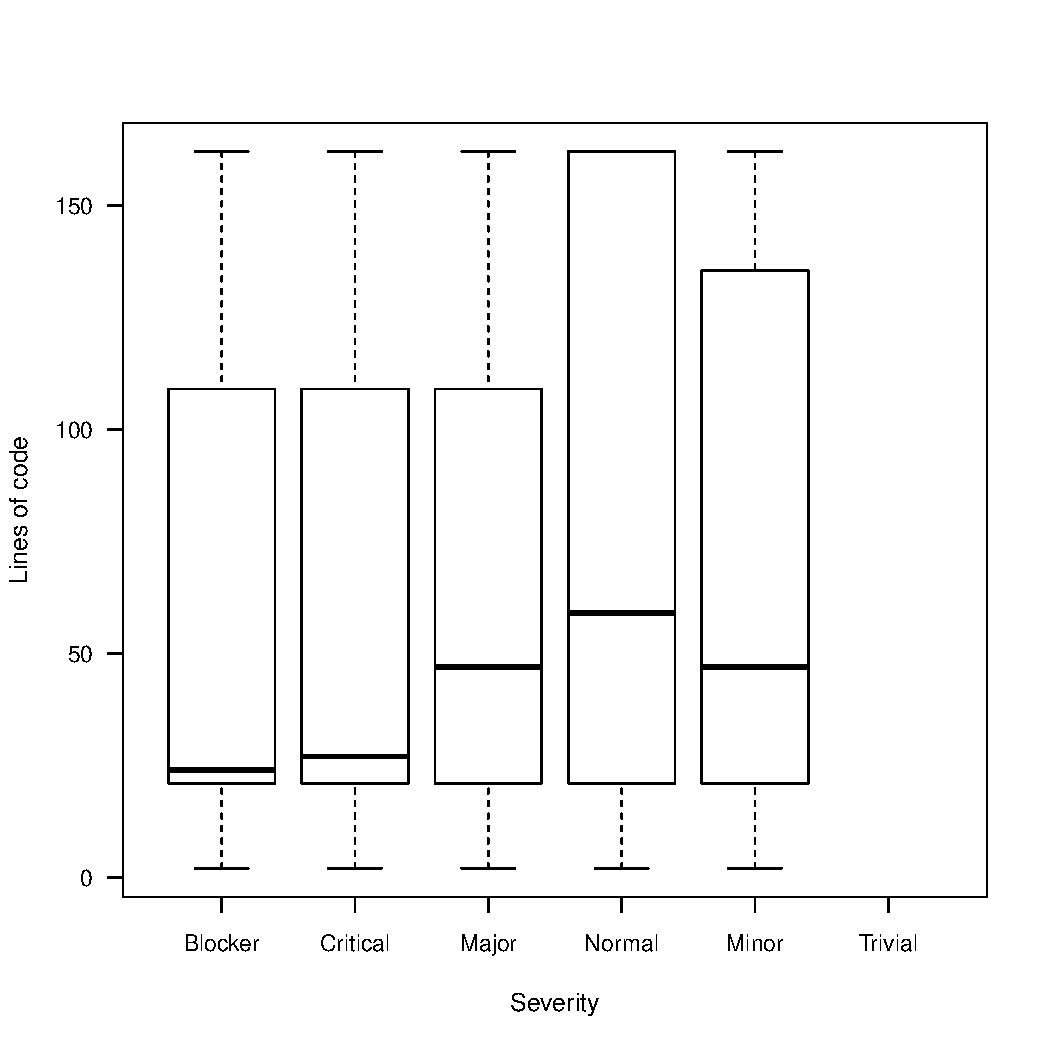
\includegraphics[width=\textwidth]{img/core-classcount-sev-boxplot.pdf}
                \caption{NOC}
                \label{fig:box-sevcore-noc}
        \end{subfigure}%
        ~ %add desired spacing between images, e. g. ~, \quad, \qquad etc. 
          %(or a blank line to force the subfigure onto a new line)
        \begin{subfigure}[b]{0.5\textwidth}
                \centering
                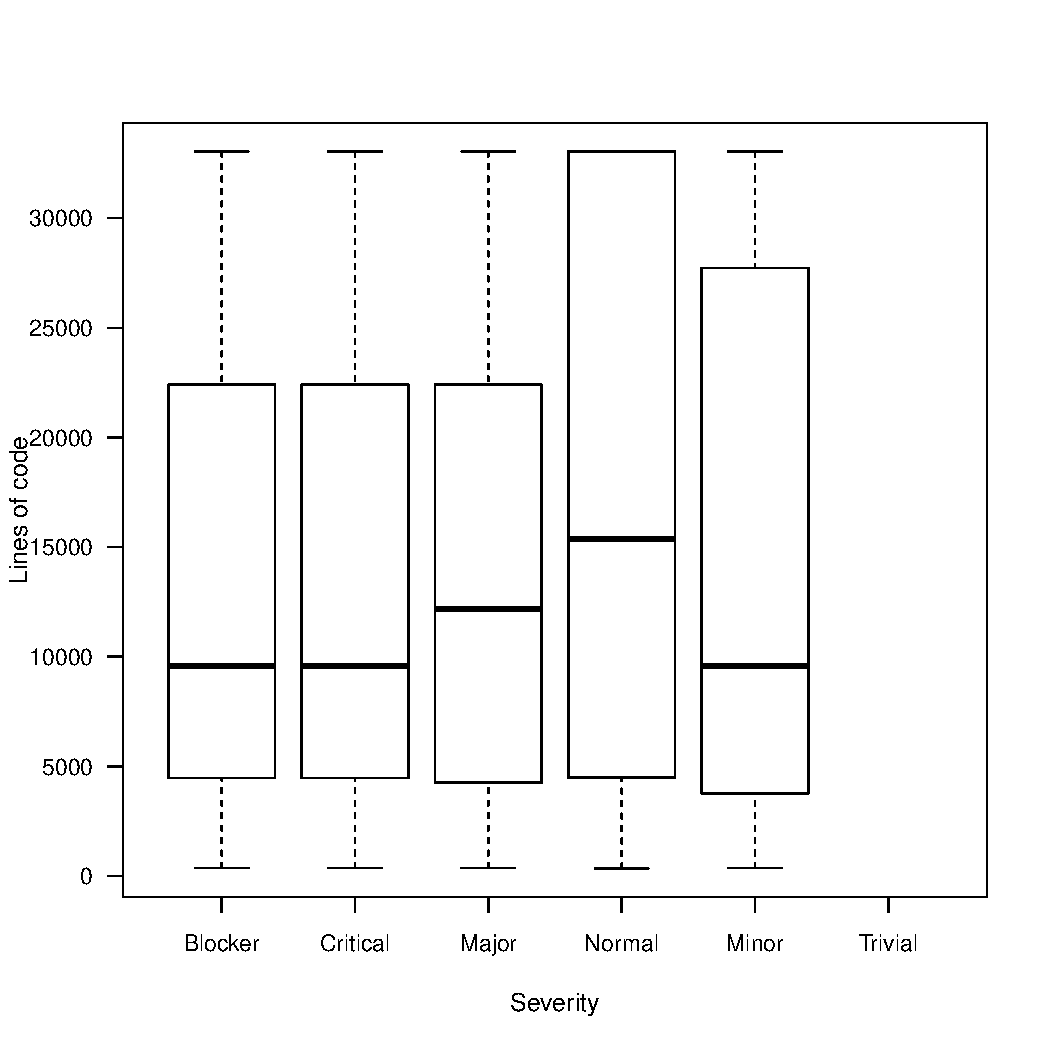
\includegraphics[width=\textwidth]{img/core-loc-sev-boxplot.pdf}
                \caption{SUMLOC}
                \label{fig:box-sevcore-sumloc}
        \end{subfigure}

        \begin{subfigure}[b]{0.5\textwidth}
                \centering
                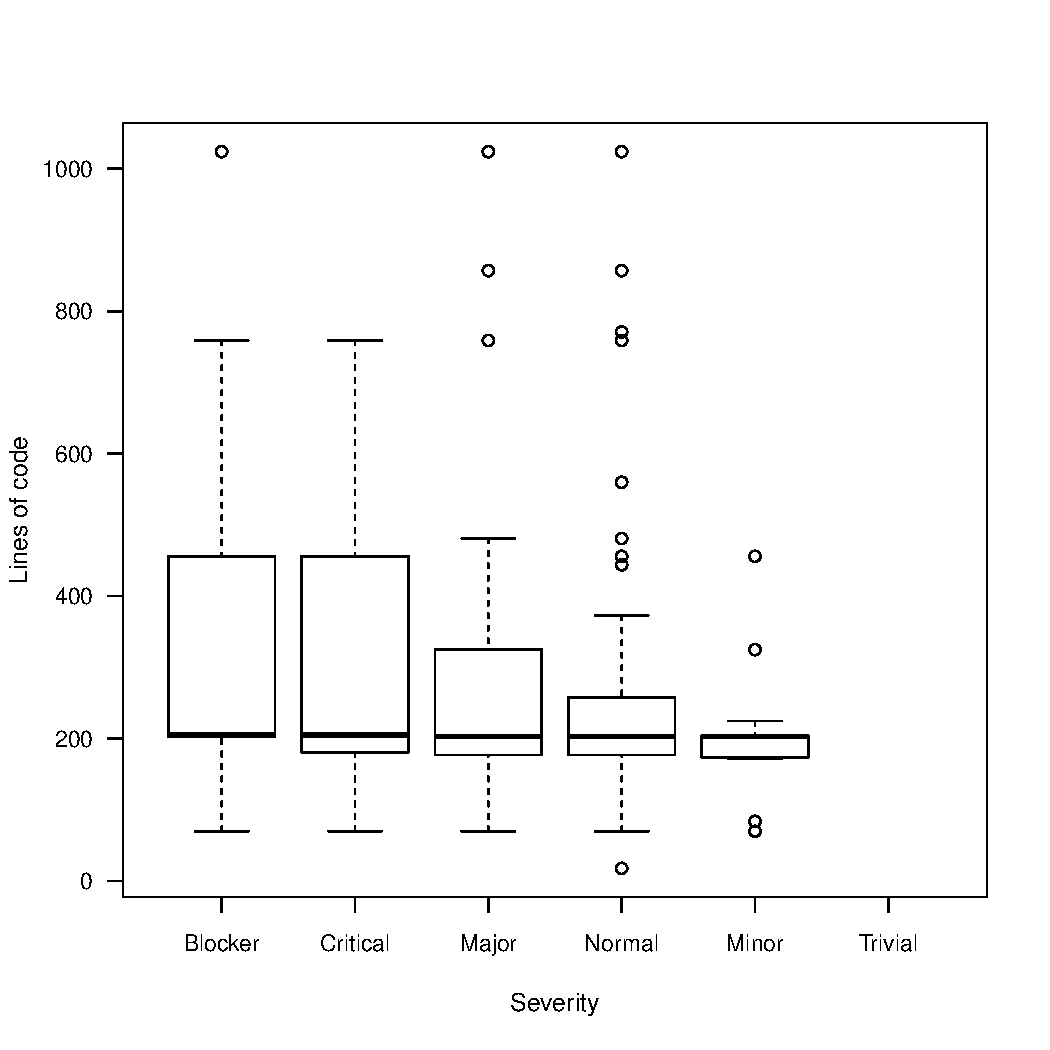
\includegraphics[width=\textwidth]{img/core-avgloc-sev-boxplot.pdf}
                \caption{AVGLOC}
                \label{fig:box-sevcore-avgloc}
        \end{subfigure}
        \caption{Distribution of package size for unique packages that are mentioned in associated bug reports for jdt.core (whiskers at 1.5 times the IQR).}
        \label{fig:packages-box-sevcore}
\end{figure}

\begin{table}[!ht]\footnotesize
	\centering
	\begin{tabular}{lrrrrrr}
		\toprule
		severity & N & min & max & mean & median & std \\
		\midrule
		NOC \\
		\midrule 
		Blocker & 57 & 2 & 162 & 55 & 24 & 52\\
		Critical & 56 & 2 & 162 & 63 & 27 & 54\\
		Major & 180 & 2 & 162 & 69 & 47 & 58\\
		Normal & 859 & 2 & 162 & 77 & 59 & 61\\\\
		\midrule
		SUMLOC \\
		\midrule
		Blocker & 57 & 369 & 33,032 & 13,201 & 9,584 & 10,049\\
		Critical & 56 & 369 & 33,032 & 14,428 & 9,584 & 10,546\\
		Major & 180 & 369 & 33,032 & 15,413 & 12,168 & 11,332\\
		Normal & 859 & 351 & 33,032 & 16,763 & 15,366 & 12,030\\\\
		\midrule
		AVGLOC \\
		\midrule
		Blocker & 57 & 70 & 1,024 & 308 & 205 & 174\\
		Critical & 56 & 70 & 759 & 283 & 205 & 172\\
		Major & 180 & 70 & 1,024 & 275 & 203 & 192\\
		Normal & 859 & 18 & 1,024 & 266 & 203 & 195\\
		\bottomrule
	\end{tabular} 
	\caption{Package size statistics for unique packages that are mentioned in associated bug reports (jdt.core). N is the number of unique packages.}
	\label{tab:package-sev-stats}
\end{table}

Since the data sets are not normal distributed and the distributions of the data sets are similar shaped (see Appendix~\ref{sub:norm:package_size}), a Wilcoxon Rank Sum test (see Section~\ref{sub:wilcoxon_rank_sum_test}) is used to compare the medians of the data sets. The null hypothesis for the Wilcoxon test states that the median values of two data sets does not differ. The alternative hypothesis for the one-sided test states $M_1 > M_2$, where $M_i$ is the median of group $i$. The results of the one-sided Wilcoxon Rank Sum test between the data sets are given in Table~\ref{tab:wilcoxon-package-sevcore}. As can be seen, only for NOC, a significant value is found (major versus normal severity). $p$-values for NOC and SUMLOC tend to be lower than for AVGLOC, with is consistent with the decrease in median and mean values that is shown when the severity becomes higher.

\begin{table}[!ht]\footnotesize
	\centering
	\begin{tabular}{llrl}
		\toprule
		data set 1 & data set 2 & $p$-value & \\
		\midrule
		NOC \\  
		\midrule
		blocker & critical & $0.1717$ & \\
		critical & major & $0.3388$ & \\
		major & normal & $0.0357$ & * \\\\
		\midrule
		SUMLOC \\  
		\midrule
		blocker & critical & $0.3335$ & \\
		critical & major & $0.3262$ & \\
		major & normal & $0.1183$ & \\\\
		\midrule
		AVGLOC \\  
		\midrule
		blocker & critical & $0.8375$ & \\
		critical & major & $0.7658$ & \\
		major & normal & $0.8766$ & \\
		\bottomrule
	\end{tabular} 
	\caption{One-sided Wilcoxon test results.}
	\label{tab:wilcoxon-package-sevcore}
\end{table}
% subsection analysis (end)

\subsection{Conclusions} % (fold)
In this section, a possible relationship between priority (or severity) and package size is investigated. Package size is defined in three ways, as described in the introduction of this section. The hypothesis for this section state that bug reports with a higher priority (or severity) are associated with packages that have a higher median value of the size metric.

Regarding the data sets for priority, the hypothesis can not be investigated due to a lack of data. Therefore,we can not conclude anything about hypothesis H1.3:

\vspace{\baselineskip}
\hypac{}
\vspace{\baselineskip}

\noindent
Also, for severity in the case of \texttt{jdt.debug}, the data is not suitable to investigate the hypothesis. In the case of \texttt{jdt.core}, sufficient data is available for categories `blocker', `critical', `major' and `normal'. The medians of the before mentioned groups are compared pairwise using a Wilcoxon Rank Sum test. The results for this test are shown in Table~\ref{tab:wilcoxon-package-sevcore}. 

Is is shown that for each test performed, the $p$-value is larger than 0.05, except for the `major' versus `normal' comparison for NOC. With these $p$-values, we accept the null hypothesis of the Wilcoxon Rank Sum test for all tests. Therefore, there is some evidence that the medians of the data sets do not differ. This leads to sufficient evidence to reject Hypothesis H1.4:

\vspace{\baselineskip}
\hypad{}
\vspace{\baselineskip}
% subsection conclusions (end)

% section analysis_of_priority_and_severity_related_to_package_size (end)

\section{Analysis of priority and severity related to class size} % (fold)
\label{sec:analysis_of_priority_and_severity_related_to_lines_of_code}
Lines of code of a class is often used as one of the most important metrics for class size. Other metrics, such as number of methods, fan-in, fan-out and depth-in-tree are sometimes also considered.

In this section, we investigate if there is a relation between the priority of a bug report and the lines of code of the corresponding classes referenced in the stack traces in that bug report. Likewise, the investigation will be done for the severity of a bug report. 

In short, the following two hypotheses of research question R1 will be discussed: 

\vspace{\baselineskip}
\hypae{}

\vspace{\baselineskip}
\hypaf{}

\vspace{\baselineskip}

\subsection{Results} % (fold)
For each bug report with a stack trace, all associated classes are determined, which all have a lines of code metric (when the source code can be found in the source code repository). A bug report can have multiple stack traces, and a stack trace can have multiple associated classes. This results in a list of pairs \emph{(report, class)}. It is possible that the same stack trace is mentioned multiple times in a bug report (for example in a quoted message). Also, a class can be mentioned multiple times in a stack trace. 

In order to make sure these duplicates do not affect the statistics, only \emph{unique} pairs \emph{(report, class)} are considered. Table~\ref{tab:loc-stats} shows some descriptive statistics for the lines of code metric of all unique pairs \emph{(report, class)} mentioned in the bug reports. These statistics are also visualised as box plots in Figure~\ref{fig:loc-boxplot}. As can be seen, \texttt{jdt.debug} and \texttt{jdt.core} both have a specific signature when it comes to lines-of-code.

\begin{table}[!ht]\footnotesize
	\centering
	\begin{tabular}{lrrrrrr}
		\toprule
		data set & N & min & max & mean & median & std \\
		\midrule
		\texttt{jdt.debug} & 74 & 13 & 2,623 & 323 & 192 & 419 \\
		\texttt{jdt.core} & 264 & 20 & 10,833 & 688 & 322 & 1,231 \\
		\bottomrule
	\end{tabular} 
	\caption{Lines of code statistics for unique classes that are mentioned in associated bug reports. N is the number of unique classes.}
	\label{tab:loc-stats}
\end{table}

\begin{figure}[!ht]
	\centering
		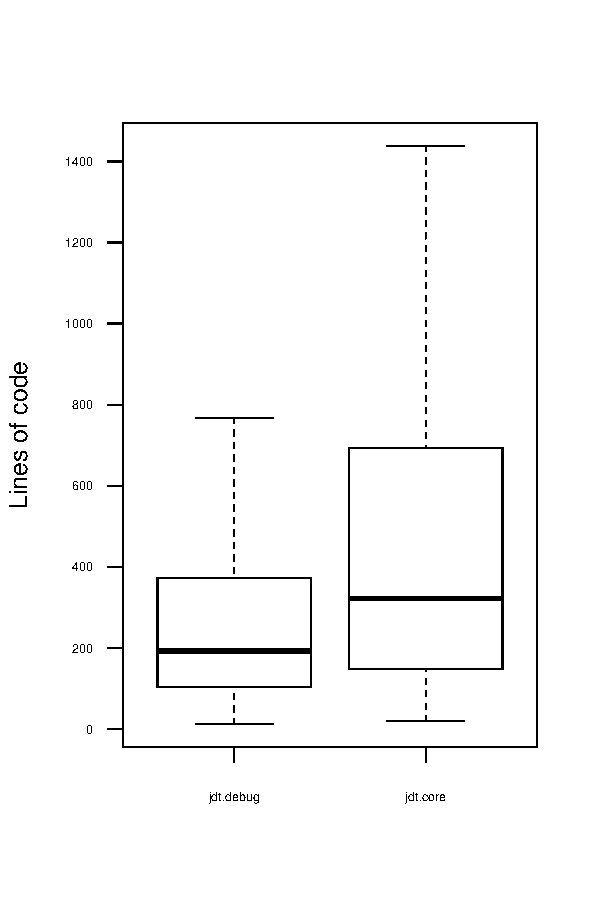
\includegraphics[width=0.7\textwidth]{img/debug-core-loc-mentioned-boxplot.pdf}
	\caption{Lines of code for unique classes that are mentioned in associated bug reports (whiskers at 1.5 times the IQR, outliers not shown).}
	\label{fig:loc-boxplot}
\end{figure}

Regarding the unique pairs \emph{(report, class)}, the tuple counts can be seen in Table~\ref{tab:prio-loc-counts}. Please note the total number of observations is higher than the number of observations in Table~\ref{tab:loc-stats}. This is of course due to the fact that the data is now also grouped on bug report. The corresponding box plots can be seen in Figure~\ref{fig:box-prio-sev}. Both for priority and severity, visually, no distinct pattern can be discovered, although median values do not seem to change much.

\begin{table}[!ht]\footnotesize
	\centering
	\begin{tabular}{lrrrrrr}
		\toprule
		 & \texttt{jdt.debug} &  & \texttt{jdt.core} &  & overall & \\
		 & all & unique & all & unique & all & unique\\
		\midrule
		P1 & 7 & 4 & 31 & 14 & 38 & 18\\
		P2 & 76 & 31 & 56 & 23 & 132 & 54\\
		P3 & 1,639 & 511 & 6,171 & 2,633 & 7,810 & 3,144\\
		P4 & 21 & 8 & 0 & 0 & 21 & 8\\
		P5 & 0 & 0 & 97 & 35 & 97 & 35\\
		\midrule
		Total & 1,743 & 554 & 6,355 & 2,705 & 8,098 & 3,259\\
		\midrule
		\\
		Blocker & 0 & 0 & 281 & 134 & 281 & 134\\
		Critical & 23 & 11 & 274 & 121 & 297 & 132\\
		Major & 348 & 79 & 1,124 & 439 & 1,472 & 518\\
		Normal & 1,329 & 454 & 4,565 & 1,966 & 5,894 & 2,420\\
		Minor & 1 & 1 & 100 & 40 & 101 & 41\\
		Trivial & 7 & 3 & 0 & 0 & 7 & 3\\
		\midrule
		Total & 1,708 & 548 & 6,344 & 2,700 & 8,052 & 3,248\\
		\bottomrule
	\end{tabular} 
	\caption{Unique \emph{(report, class)} pair-counts.}
	\label{tab:prio-loc-counts}
\end{table}

\begin{figure}
        \begin{subfigure}[b]{0.5\textwidth}
                \centering
                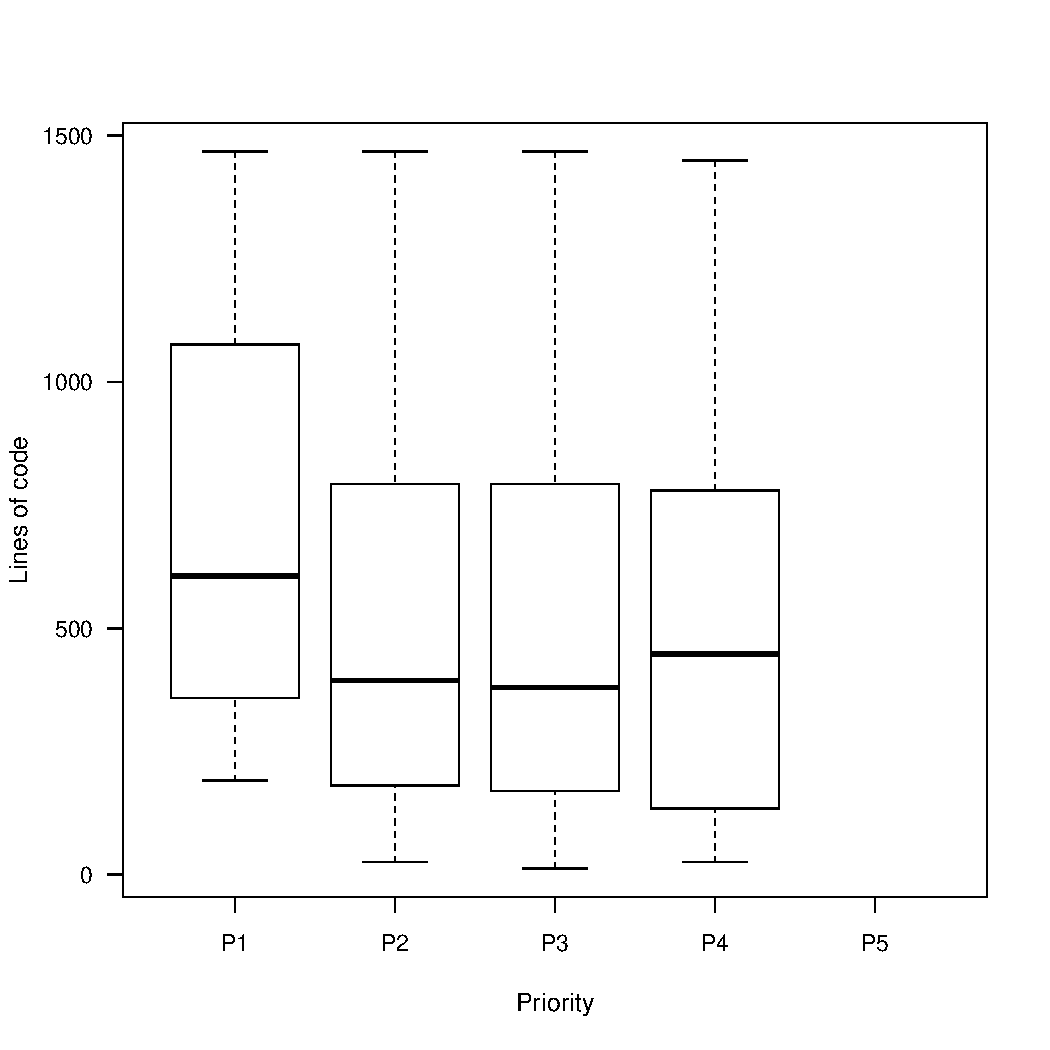
\includegraphics[width=\textwidth]{img/debug-unique-prio-boxplot.pdf}
                \caption{Priority --- jdt.debug}
                \label{fig:box-prio-debug}
        \end{subfigure}%
        ~ %add desired spacing between images, e. g. ~, \quad, \qquad etc. 
          %(or a blank line to force the subfigure onto a new line)
        \begin{subfigure}[b]{0.5\textwidth}
                \centering
                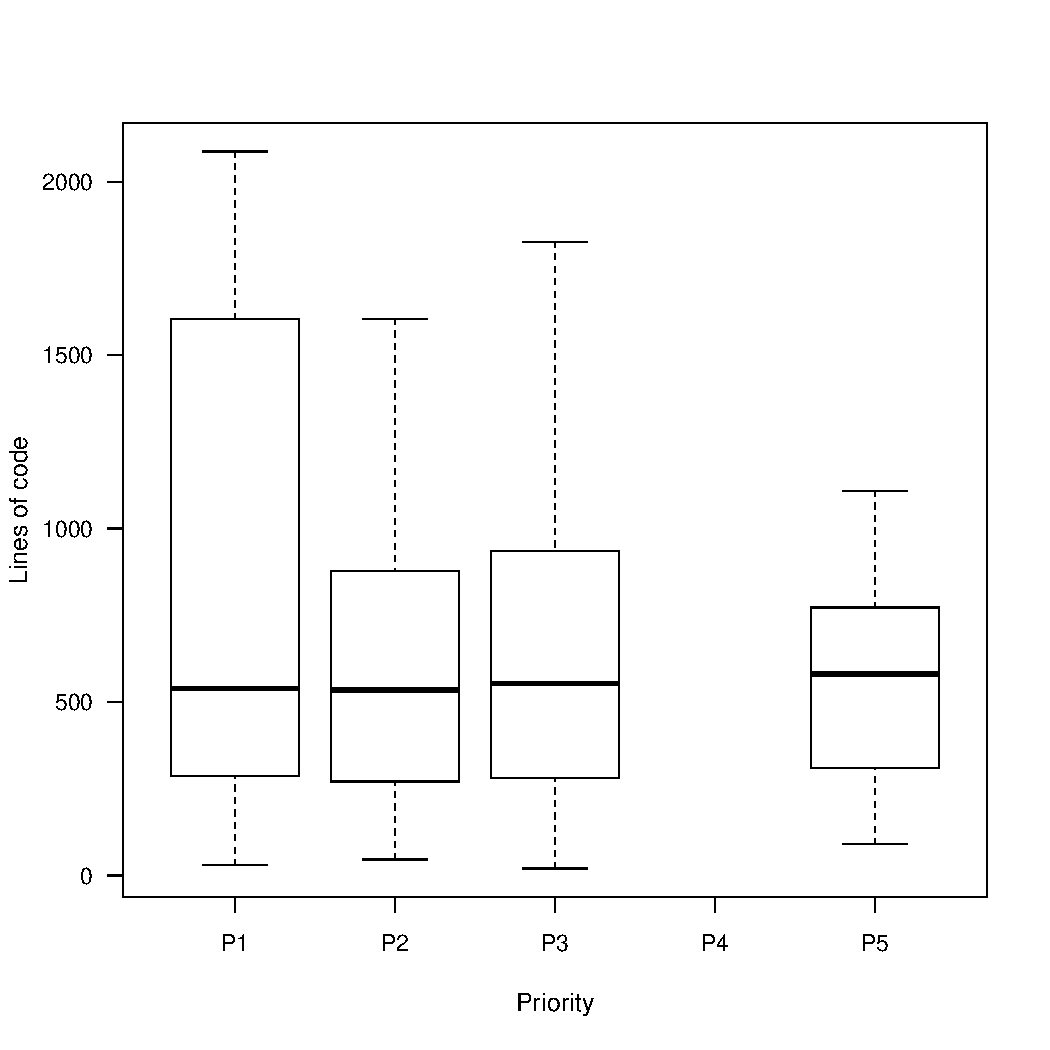
\includegraphics[width=\textwidth]{img/core-unique-prio-boxplot.pdf}
                \caption{Priority --- jdt.core}
                \label{fig:box-prio-core}
        \end{subfigure}

        \begin{subfigure}[b]{0.5\textwidth}
                \centering
                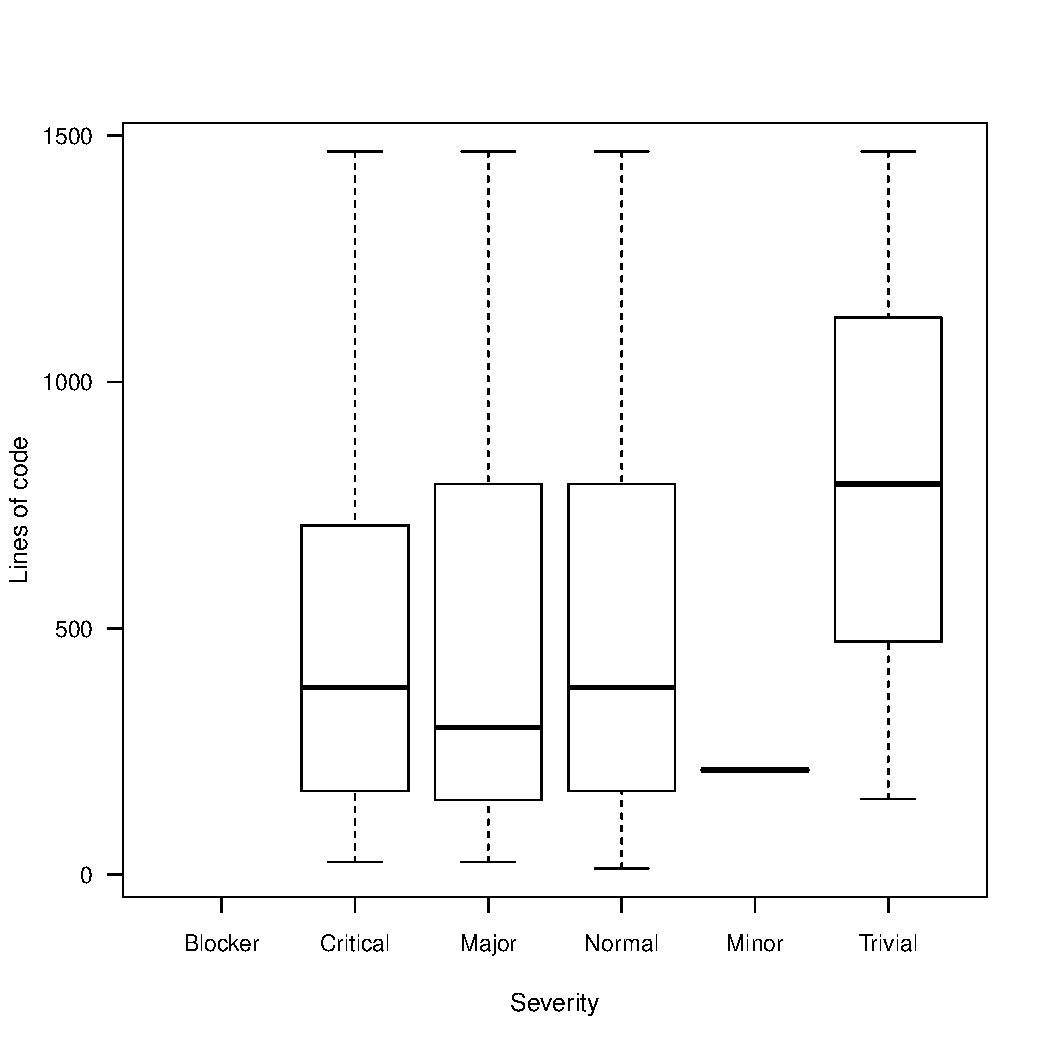
\includegraphics[width=\textwidth]{img/debug-unique-sev-boxplot.pdf}
                \caption{Severity --- jdt.debug}
                \label{fig:box-sev-debug}
        \end{subfigure}
        ~ %add desired spacing between images, e. g. ~, \quad, \qquad etc. 
          %(or a blank line to force the subfigure onto a new line)
        \begin{subfigure}[b]{0.5\textwidth}
                \centering
                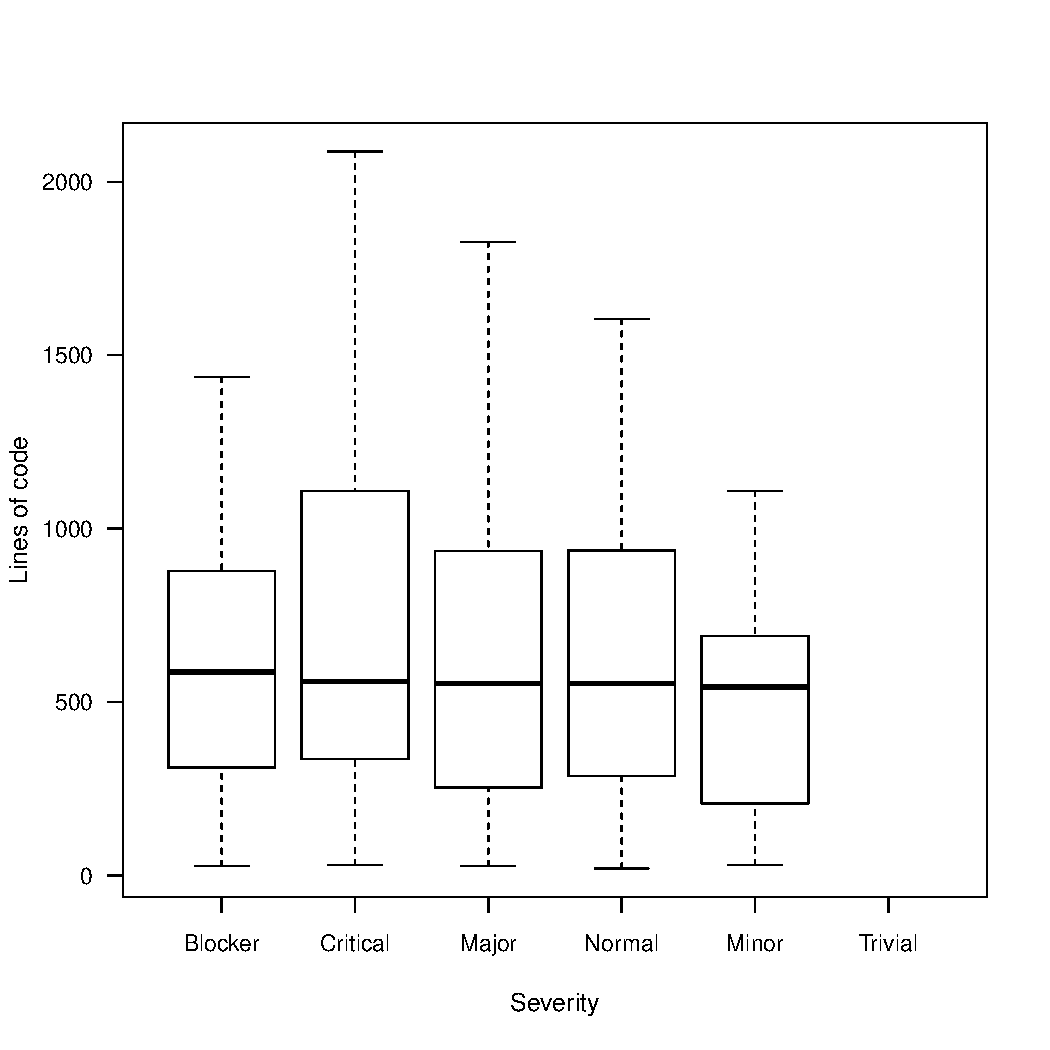
\includegraphics[width=\textwidth]{img/core-unique-sev-boxplot.pdf}
                \caption{Severity --- jdt.core}
                \label{fig:box-sev-core}
        \end{subfigure}
        \caption{Distribution of class size for unique classes that are mentioned in associated bug reports (whiskers at 1.5 times the IQR, outliers not shown).}
        \label{fig:box-prio-sev}
\end{figure}
% subsection results (end)

\subsection{Analysis} % (fold)
In order to investigate whether there is a relation between priority (or severity) and class size, a pairwise comparison of the median values of each data set needs to be made. For priority, P1 and P2 are compared, P2 and P3, et cetera. For severity, `blocker' and `critical' are compared, `critical' and `major', et cetera.

Table~\ref{tab:prio-loc-counts} shows that for \texttt{jdt.debug}, no bug reports with priority P5 are present. The same applies to \texttt{jdt.core} and priority P4. For \texttt{jdt.debug}, the number of data points is also low (4) for priority P1. Regarding the severity, a similar pattern is present. For \texttt{jdt.debug}, a low amount of data points is seen for severities `blocker' (0), `minor' (1) and `trivial' (3), and for \texttt{jdt.core} this applies to `trivial' (0). This is consistent with the research performed in \cite{Lamkanfi2010}, who found that most bug reports get assigned the default value for priority and severity. It is tempting to combine both \texttt{jdt.debug} and \texttt{jdt.core} into one data set to overcome the sample size issues. However, Figure~\ref{fig:loc-boxplot} and Table~\ref{tab:loc-stats} show the distribution of both data sets is quite different. 

This means not all possible pairwise comparisons can be performed. When a minimum sample size of 20 is taken into account, the only logical investigation is the relation between severity and lines of code for the \texttt{jdt.core} project. With this data set, four comparisons can be made (`blocker' vs `critical', `critical' vs `major', `major' vs `normal', `normal' vs `minor'). Using these four comparisons, a possible relationship between the two dimensions (severity and lines of code) can be shown.

The median line of code values of the five datasets for \texttt{jdt.core} are shown in Table~\ref{tab:statistics-invg}. Figure~\ref{fig:box-prio-sev} shows the box plots for the data sets.

\begin{table}[!ht]\footnotesize
	\centering
	\begin{tabular}{lrrrrrr}
		\toprule
		severity & N & min & max & mean & median & std \\
		\midrule
		Blocker & 134 & 27 & 8,218 & 857 & 586 & 1,052\\
		Critical & 121 & 29 & 8,218 & 1,046 & 559 & 1,507\\
		Major & 439 & 27 & 10,833 & 887 & 553 & 1,228\\
		Normal & 1,966 & 20 & 10,833 & 974 & 553 & 1,494\\
		Minor & 40 & 30 & 3,297 & 605 & 544 & 640\\
		\bottomrule
	\end{tabular} 
	\caption{Lines of code statistics for data under investigation (jdt.core). N is the number of measurements.}
	\label{tab:statistics-invg}
\end{table}

Since the data sets are not normally distributed and the distributions of the data sets are similar shaped (see Appendix~\ref{sub:norm:package_size}), a Wilcoxon Rank Sum test (see Section~\ref{sub:wilcoxon_rank_sum_test}) is used to compare the medians of the data sets. The null hypothesis for the Wilcoxon test states that the median values of two data sets does not differ. The alternative hypothesis for the one-sided test states $M_1 > M_2$, where $M_i$ is the median of group $i$. The results of the one-sided Wilcoxon Rank Sum test between the data sets are given in Table~\ref{tab:wilcoxon-sev-core}. The $p$-values do not show any significant results that might lead to suspecting a shift in median time-to-fix, which corresponds with the data shown in Figure~\ref{fig:box-prio-sev}(d).

\begin{table}[!ht]\footnotesize
	\centering
	\begin{tabular}{llrl}
		\toprule
		data set 1 & data set 2 & $p$-value & \\
		\midrule
		blocker & critical & $0.5575$ & \\
		critical & major & $0.8679$ & \\
		major & normal & $0.3497$ & \\
		normal & minor & $0.9094$ & \\
		\bottomrule
	\end{tabular} 
	\caption{One-sided Wilcoxon test results for jdt.core.}
	\label{tab:wilcoxon-sev-core}
\end{table}

% subsection analysis (end)
\subsection{Conclusions} % (fold)
In this section, a possible relationship between priority (or severity) and class size is investigated. As a hypothesis it is stated that bug reports with a higher priority (or severity) are associated with classes mentioned in bug report stack traces that have a higher median value of the lines of code metric.

Regarding the data sets for priority, the hypothesis can not be investigated due to a lack of data. Therefore, we cannot conclude anything about hypothesis H1.5:

\vspace{\baselineskip}
\hypae{}
\vspace{\baselineskip}

\noindent
Also, for severity in the case of \texttt{jdt.debug}, the data is also not suitable to investigate the hypothesis. For severity in the case of \texttt{jdt.core}, sufficient data is available for categories `blocker', `critical', `major', `normal' and `minor'. The medians of the before mentioned groups are compared pairwise using a Wilcoxon Rank Sum test. The results for this test are shown in Table~\ref{tab:wilcoxon-sev-core}. Is is shown that for each test performed, the $p$-value is larger than 0.05. With these $p$-values, we accept the null hypothesis of the Wilcoxon Rank Sum test for all tests. Therefore, there is no evidence that the medians of the data sets differ. We therefore reject hypothesis H1.6:

\vspace{\baselineskip}
\hypaf{}
\vspace{\baselineskip}
 
% subsection conclusions (end)

% section analysis_of_priority_and_severity_related_to_lines_of_code (end)

\section{Summary of results} % (fold)
\label{sec:priosev-summary_of_results}
This chapter showed the results and analysis for research question R1, as described in Chapter~\ref{sec:analysis:priority_and_severity}:

\vspace{\baselineskip}
\questiona{}
\vspace{\baselineskip}

\noindent
First, it was investigated whether the presence of one or more stack traces in a bug report corresponds with a higher priority (or severity) of the bug report. For priority, some evidence is found for \texttt{jdt.debug}, with strong evidence for \texttt{jdt.core}. This gives enough evidence to partially accept hypothesis H1.1. For severity, the number of bug reports with a higher than normal severity increases when a stack trace is present. Also, the number of bug reports with a lower than normal severity decreases when a stack trace is present. Therefore hypothesis H1.2 is accepted.

The second investigation is about a possible relation between priority (and severity) and package size. Three definitions of package size are investigated. For priority, not enough data is present, so it is not possible to state anything regarding hypothesis H1.3. For severity, sufficient data is only available for \texttt{jdt.core}. For this case, there is no evidence of a relation between severity and package size. Concluding, there is some evidence to reject hypothesis H1.4.

Finally, the second investigation is repeated for a finer granularity: class size. For priority, there is no sufficient data available. Therefore it is not possible to state anything regarding hypothesis H1.5. For severity, sufficient data is available for \texttt{jdt.core}, but there is no evidence that the medians of the data sets differ. Concluding, there is some evidence to reject hypothesis H1.6.

The next chapter investigates whether there is a relation between bug reports and the time-to-fix of a bug.
% section summary_of_results (end)
% chapter results_priority_and_severity (end)
%!TEX root = thesis.tex

\chapter{Results: Time-to-fix} % (fold)
\label{cha:results_time_to_fix}

In this chapter, the second research question and the accompanying hypotheses are investigated, as defined in Section~\ref{sec:research_questions}:

\vspace{\baselineskip}
\questionb{}

In order to answer this question, the following hypothesis are stated:

\vspace{\baselineskip}
\hypba{}

\vspace{\baselineskip}
\hypbb{}

\vspace{\baselineskip}
\hypbc{}

\section{Overview} % (fold)
All investigations are split into three parts: 
\begin{inparaenum}[(1)]
\item \textbf{results}, describing the direct results of the study and showing some descriptive statistics,
\item \textbf{analysis}, analysing the results of the study, and
\item \textbf{conclusions}, which evaluates the hypothesis.
\end{inparaenum}

In Section \ref{sec:analysis_of_ttf_vs_presence_of_stack_trace_in_bug_report}, it is investigated whether the time-to-fix of a bug decreases when a stack trace is present. Section \ref{sec:analysis_of_ttf_version_stack_trace_position_in_comments} investigates if the position of a stack trace in the bug report has influence on the time-to-fix. Section \ref{sec:correlation_analysis_between_loc_and_ttf} investigates the correlation between class size and the time-to-fix of the corresponding bug reports.

Finally, all results found in the previous mentioned sections are summarised in Section \ref{sec:ttf_summary_of_results}.

% section overview (end)

\section{Analysis of time-to-fix versus presence of stack traces in bug report} % (fold)
\label{sec:analysis_of_ttf_vs_presence_of_stack_trace_in_bug_report}
We expect that the time-to-fix of a bug decreases when a stack trace is present in the bug report. With this stack trace, it might be easier to reproduce the bug and to know where to look in the source code. This is also shown by Schr\"{o}ter \emph{et al.} in \cite{Schroter2010}. Therefore, the first hypothesis of research question R1 is investigated in this section:

\vspace{\baselineskip}
\hypba{}

\subsection{Results} % (fold)
All bug reports from \texttt{jdt.debug} marked with status \textsc{verified} and resolution \textsc{fixed} are split into two groups: 

\begin{enumerate*}
	\item bug reports that include a stack trace in one or more of the comments, and
	\item bug reports that do not include a stack trace.
\end{enumerate*}

All bugs from \texttt{jdt.core} are discarded, since only a specific subset of bugs is imported (the bugs that probably mention one or more exceptions). This means this specific data set is expected to have a certain bias. Although not all imported bugs do contain an actual exception, which might make the data set usable after all, we decided to not use this data set in our investigations.

For each bug report, the time-to-fix is calculated. All reports with a time-to-fix of $0$ days are removed from the data sets, since these reports probably are only created for administrative reasons.

In Table~\ref{tab:ttf_stats}, some descriptive statistics of the resulting data sets are shown, such as mean, standard deviation, minimum value, maximum value and median. The data sets are also plotted as box plots in Figure~\ref{fig:ttf_with_without_stacktrace}.

\begin{table}[!ht]\footnotesize
	\centering
	\begin{tabular}{lrrrrrr}
		\toprule
		data set & N & min & max & mean & median & std \\
		\midrule
		\texttt{jdt.debug} with stack trace & 180 & 1 & 644 & 62 & 14 & 108 \\
		\texttt{jdt.debug} without stack trace & 2,108 & 1 & 3,137 & 98 & 18 & 232 \\
		\bottomrule
	\end{tabular} 
	\caption{Time-to-fix (in days) statistics of the jdt.debug. N is the number of measurements.}
	\label{tab:ttf_stats}
\end{table}
 
\begin{figure}[!ht]
	\centering
		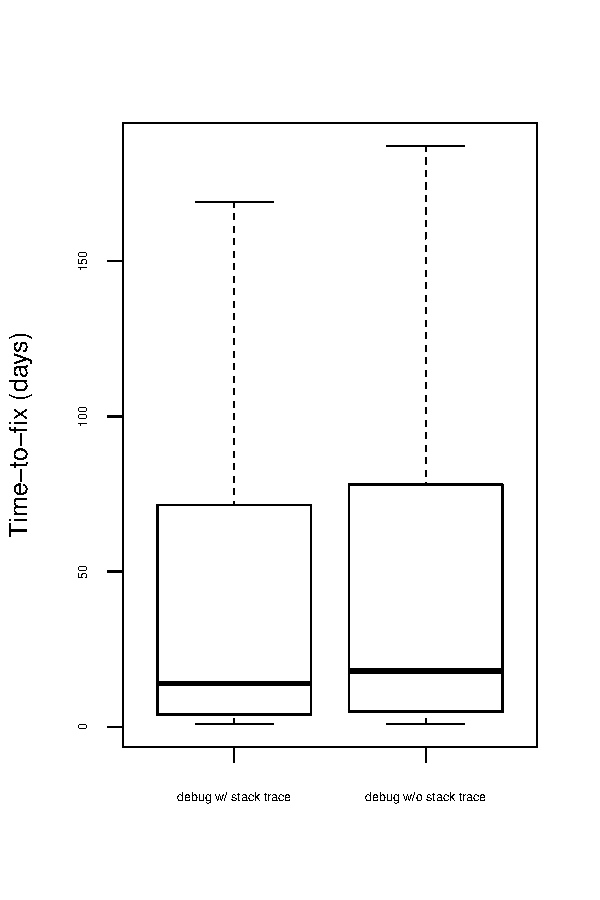
\includegraphics[width=0.7\textwidth]{img/ttf_with_without_stacktrace.pdf}
	\caption{Comparison between bug reports with and without a stack trace (whiskers at 1.5 times the IQR).}
	\label{fig:ttf_with_without_stacktrace}
\end{figure}

% subsection results (end)

\subsection{Analysis} % (fold)
We are investigating if the time-to-fix of a bug decreases when a stack trace is present in the bug report. In order to do this, the median time-to-fix for data sets with and without stack traces are compared. This is done pairwise for the \texttt{jdt.debug} project.

Table~\ref{tab:ttf_stats} shows that for \texttt{jdt.debug}, the median time-to-fix decreases when a stack trace is present. The mean time-to-fix decreases by five weeks when a stack trace is present.

Since the data sets are not normal distributed and the distributions of the data sets are similar shaped (see Appendix~\ref{sub:norm:presence_of_stack_trace}), the Wilcoxon Rank Sum test (see Section~\ref{sub:wilcoxon_rank_sum_test}) is used to compare the medians of the data sets.
The null hypothesis for the Wilcoxon test states that the median values of two data sets does not differ. The alternative hypothesis for the one-sided test states $M_1 < M_2$, where $M_i$ is the median of group $i$. 

The $p$-value for this one-sided Wilcoxon Rank Sum test for \texttt{jdt.debug} is:

\[
	p = 0.1277
\]

% subsection analysis (end)

\subsection{Conclusions} % (fold)
When looking at the time-to-fix statistics in Table~\ref{tab:ttf_stats}, it can be noted the median time-to-fix decreases when a stack trace is mentioned in a bug report. Also, the mean time-to-fix decreases by five weeks when a stack trace is present. 

With respect to the mean time-to-fix, a higher standard deviation can be noticed in the data sets without stack traces. This, combining with a relative higher number of measurements (and thus probably a higher number of outliers, since the distributions are similar), causes the increase in time-to-fix.

Based on the results of the one-sided Wilcoxon test, the $p$-value for \texttt{jdt.debug} does not satisfy $p < \alpha$, where $\alpha = 0.05$. Therefore we conclude that there is no evidence that the median time-to-fixes in bug reports with a stack trace differs from bug reports without a stack trace. However, the descriptive statistics are promising, showing that both mean (over a month) and median (4 days) time-to-fix values decrease significantly when a stack trace is present. We therefore partially accept hypothesis H2.1:

\vspace{\baselineskip}
\hypba{}

% subsection conclusions (end)
% section analysis_of_ttf_vs_presence_of_stack_trace_in_bug_report (end)

\section{Analysis of time-to-fix versus stack trace position in comments} % (fold)
\label{sec:analysis_of_ttf_version_stack_trace_position_in_comments}
The previous section showed there is no evidence for a decrease in time-to-fix when a stack trace is present. However, could the time-to-fix be positively affected (i.e., decrease) when the stack trace is present in the \emph{first} comment of a bug report? This way, the stack trace is immediately available to the bug traiger, and can therefore be used in the assessment of the bug report. In this section, the second hypothesis of research question R2 is investigated:

\vspace{\baselineskip}
\hypbb{}

\subsection{Results} % (fold)
All bug reports with a stack trace from \texttt{jdt.core} and \texttt{jdt.debug} marked with status \textsc{verified} and resolution \textsc{fixed} are split into two groups: 

\begin{enumerate*}
	\item bug reports with one or more stack traces in the first comment, and
	\item bug reports with one or more stack traces in non-first comment(s).
\end{enumerate*}

For each bug report, the time-to-fix is calculated. All reports with a time-to-fix of $0$ days are removed from the data sets, since these reports probably are only created for administrative reasons.

In Table~\ref{tab:ttf_pos_stats}, some descriptive statistics of the resulting data sets are shown, such as mean, standard deviation, minimum value, maximum value and median. The data sets are also plotted as box plots in Figure~\ref{fig:ttf_pos_stats}.

\begin{table}[!ht]\footnotesize
	\centering
	\begin{tabular}{lrrrrrr}
		\toprule
		data set & N & min & max & mean & median & std \\
		\midrule
		\texttt{jdt.debug} with stack traces in first comment & 116 & 1 & 1,744 & 60 & 9 & 178 \\
		\texttt{jdt.debug} with stack traces in non-first comment(s) & 23 & 1 & 1,130 & 137 & 40 & 209 \\
		\texttt{jdt.core} with stack traces in first comment & 186 & 1 & 644 & 66 & 12 & 119 \\
		\texttt{jdt.core} with stack traces in non-first comment(s) & 52 & 1 & 285 & 57 & 29 & 87 \\
		overall with stack traces in first comment & 302 & 1 & 1,744 & 62 & 12 & 157 \\
		overall with stack traces in non-first comment(s) & 75 & 1 & 1,130 & 112 & 32 & 184 \\
		\bottomrule
	\end{tabular} 
	\caption{Time-to-fix (in days) statistics of the data. N is the number of measurements.}
	\label{tab:ttf_pos_stats}
\end{table}
 
\begin{figure}[!ht]
	\centering
		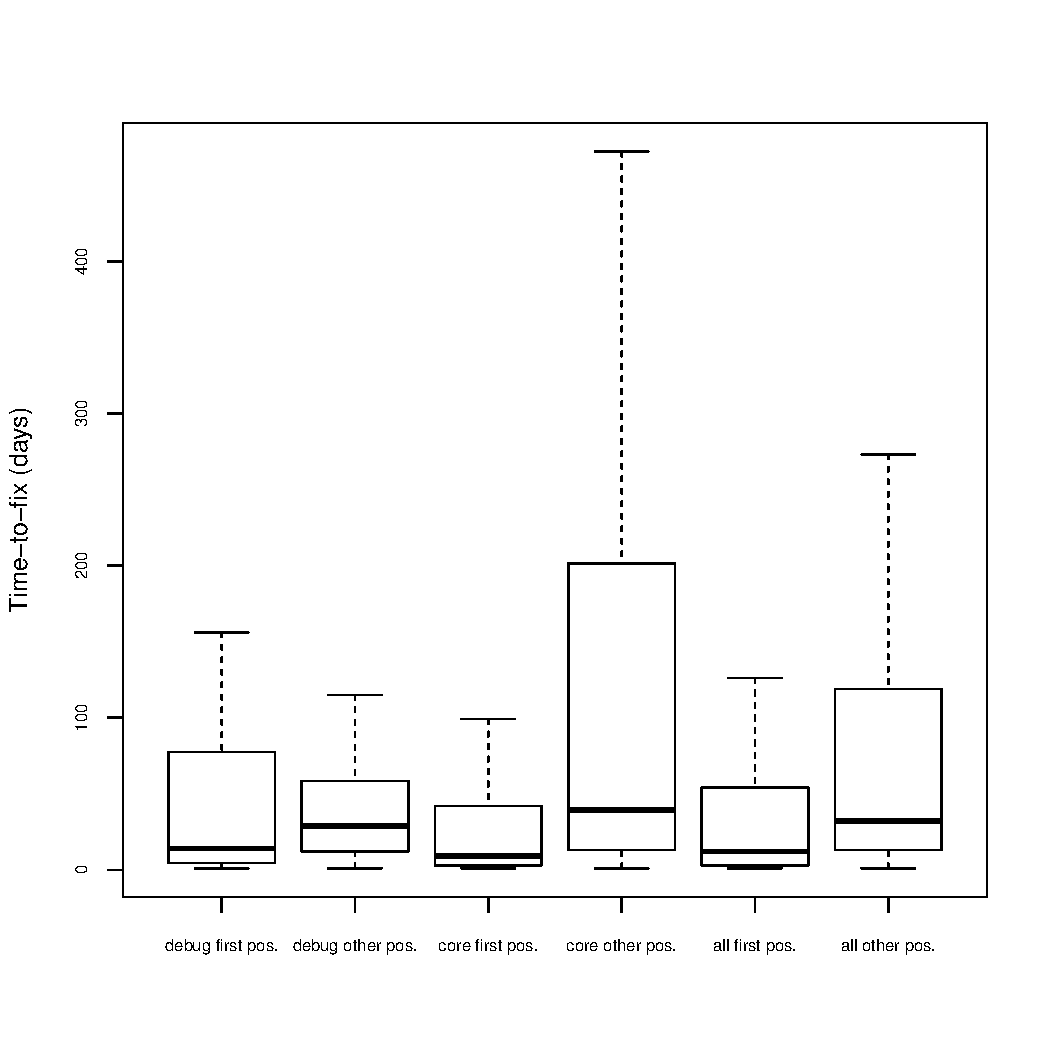
\includegraphics[width=1\textwidth]{img/ttf_stacktrace_pos.pdf}
	\caption{Comparison between bug reports with and without a stack trace (whiskers at 1.5 times the IQR).}
	\label{fig:ttf_pos_stats}
\end{figure}

% subsection results (end)

\subsection{Analysis} % (fold)
We are investigating if the time-to-fix of a bug report that includes one or more stack traces \emph{decreases} when a stack trace is present in the first comment of the bug report. In order to do this, the median time-to-fix for these data sets are compared:

\begin{itemize*}
	\item \texttt{jdt.debug} reports with stack traces in the first comment versus \texttt{jdt.debug} reports with stack traces in non-first comments
	\item \texttt{jdt.core} reports with stack traces in the first comment versus \texttt{jdt.core} reports with stack traces in non-first comments
	\item combined bug reports from \texttt{jdt.debug} and \texttt{jdt.core} with stack traces in the first comment versus combined bug reports from \texttt{jdt.debug} and \texttt{jdt.core} with stack traces in non-first comments
\end{itemize*}

Table~\ref{tab:ttf_pos_stats} shows that for all data sets, the median time-to-fix decreases when a stack trace is present in the first comment. In all three measures, the mean time-to-fix decreases by two to four weeks. 

Since the data sets are not normal distributed and the distributions of the data sets are similar shaped (see Appendix~\ref{sub:norm:presence_of_stack_trace}), the Wilcoxon Rank Sum test (see Section~\ref{sub:wilcoxon_rank_sum_test}) is used to compare the medians of the data sets.
The null hypothesis for the Wilcoxon test states that the median values of two data sets does not differ. The alternative hypothesis for the one-sided test states $M_1 < M_2$, where $M_i$ is the median of group $i$. The results of the one-sided Wilcoxon Rank Sum test between the data sets are given in Table~\ref{tab:wilcoxon_pos}.

\begin{table}[!ht]\footnotesize
	\centering
	\begin{tabular}{llrl}
		\toprule
		data set 1 & data set 2 & $p$-value & \\
		\midrule
		\texttt{jdt.debug} w/ st. in first comment & \texttt{jdt.debug} w/ st. in other comment & $0.1271$ & \\
		\texttt{jdt.core} w/ st. in first comment & \texttt{jdt.core} w/ st. in other comment & $< 0.001$ & *** \\
		overall  w/ st. in first comment & overall w/ st. in other comment & $< 0.001$ & *** \\
		\bottomrule
	\end{tabular} 
	\caption{One-sided Wilcoxon test results.}
	\label{tab:wilcoxon_pos}
\end{table}

% subsection analysis (end)

\subsection{Conclusions} % (fold)
When looking at the time-to-fix statistics in Table~\ref{tab:ttf_pos_stats}, it can be noted the median time-to-fix decreases decreases when a stack trace is present in the first comment. Based on the results of the one-sided Wilcoxon test in Table~\ref{tab:wilcoxon_pos}, the $p$-values for \texttt{jdt.core} and the overall data set satisfy $p < \alpha$, where $\alpha = 0.001$, resulting in a highly significant result. However, for \texttt{jdt.debug}, no statistically significant $p$-value is found, which is probably due to the fact that the number of data points is limited.

In conclusion, the null hypothesis stating the difference in medians of the two data sets is a coincidence is rejected for \texttt{jdt.core} and the overall data set. Therefore, there is evidence that the time-to-fix for bugs decreases when a stack trace is present in the first comment, compared to bug reports with a stack trace in the non-first comment. We therefore accept hypothesis H2.2:

\vspace{\baselineskip}
\hypbb{}

\noindent
This is consistent with the results of Schr\"{o}ter \emph{et al.} \cite{Schroter2010}. They found strong evidence that bug reports that include one or more stack traces do indeed have a shorter lifetime. Regarding stack trace position in the bug report, they found that 70\% of the bugs were fixed in a stack frame from the \emph{first} stack trace in the bug report.

% subsection conclusions (end)

% section analysis_of_ttf_version_stack_trace_position_in_comments (end)

\section{Correlation analysis between class size and time-to-fix} % (fold)
\label{sec:correlation_analysis_between_loc_and_ttf}
When one or more stack traces are present in comments of a bug report, it is possible to relate each bug report to one or more source classes. A larger class size might point to less understandable code, hence to a higher time-to-fix for a bug. In this section, it will be investigated if there is a relation between class size and time-to-fix of a bug report. The following hypothesis of research question R2 will be discussed:

\vspace{\baselineskip}
\hypbc{}

\subsection{Results} % (fold)
Table~\ref{tab:ttf_loc_stats} contains all 29 classes in both the \texttt{jdt.debug} and \texttt{jdt.core} projects that are matched to at least ten bug reports with status \textsc{verified} and resolution \textsc{fixed}. We match to at least ten bug reports, so we are sure the descriptive statistics are based on sufficient data. All bug reports with a fix time of 0 days are again removed from the results. For each class, the number of matching bug reports, the median time-to-fix of these bug reports, and the lines of code of the class are shown.

The total number of distinct classes in all stack traces is 2,533, but only 339 (13\%) from these classes are available as actual source code for \texttt{jdt.debug} or \texttt{jdt.core}. All other classes refer to classes from external libraries or the Java core. From these 339 classes, only the 29 (8\%, 1\% overall) classes shown in Table~\ref{tab:ttf_loc_stats} are mentioned in ten or more bug reports.

\begin{table}[!ht]\footnotesize
	\centering
	\begin{tabular}{lr|rrrrrr}
		\toprule
		class & LOC & N & min & max & mean & med. & std \\
		\midrule
		\verb|core.dom.ASTParser| & 593 & 12 & 3 & 366 & 53 & 14 & 106 \\
		\verb|core.JavaCore| & 1,309 & 14 & 2 & 366 & 105 & 57 & 116 \\
		\verb|core.search.SearchEngine| & 286 & 20 & 1 & 1,161 & 160 & 34 & 288 \\
		\verb|internal.codeassist.CompletionEngine| & 10,833 & 11 & 1 & 449 & 54 & 7 & 132 \\
		\verb|i.comp.ast.AbstractMethodDeclaration| & 364 & 14 & 1 & 149 & 18 & 8 & 38 \\
		\verb|i.comp.ast.CompilationUnitDeclaration| & 559 & 19 & 1 & 149 & 18 & 7 & 35 \\
		\verb|i.comp.ast.MethodDeclaration| & 217 & 14 & 1 & 244 & 29 & 7 & 64 \\
		\verb|i.comp.ast.TypeDeclaration| & 1,108 & 25 & 1 & 244 & 26 & 8 & 55 \\
		\verb|i.comp.Compiler| & 580 & 36 & 1 & 150 & 26 & 9 & 43 \\
		\verb|i.comp.lookup.ClassScope| & 998 & 11 & 1 & 150 & 33 & 11 & 51 \\
		\verb|i.comp.lookup.CompilationUnitScope| & 654 & 16 & 1 & 150 & 25 & 9 & 43 \\
		\verb|i.comp.lookup.LookupEnvironment| & 1,015 & 16 & 1 & 150 & 26 & 10 & 43 \\
		\verb|i.comp.lookup.Scope| & 3,297 & 12 & 1 & 150 & 31 & 8 & 49 \\
		\verb|i.core.BinaryType| & 740 & 11 & 1 & 1,744 & 201 & 40 & 514 \\
		\verb|i.core.builder.AbstractImageBuilder| & 641 & 14 & 1 & 147 & 26 & 12 & 39 \\
		\verb|i.core.builder.JavaBuilder| & 639 & 16 & 1 & 147 & 24 & 10 & 37 \\
		\verb|i.core.CompilationUnit| & 877 & 35 & 1 & 449 & 60 & 9 & 105 \\
		\verb|i.core.CompilationUnitProblemFinder| & 162 & 19 & 1 & 253 & 41 & 9 & 71 \\
		\verb|i.core.JavaElement| & 534 & 29 & 1 & 1,744 & 125 & 36 & 324 \\
		\verb|i.core.JavaModelManager| & 3,749 & 13 & 5 & 243 & 59 & 30 & 78 \\
		\verb|i.core.JavaModelOperation| & 553 & 34 & 1 & 266 & 56 & 13 & 84 \\
		\verb|i.core.JavaProject| & 2,087 & 19 & 1 & 253 & 65 & 30 & 84 \\
		\verb|i.core.Openable| & 311 & 24 & 1 & 449 & 71 & 11 & 117 \\
		\verb|i.core.ReconcileWorkingCopyOperation| & 173 & 22 & 1 & 253 & 47 & 8 & 80 \\
		\verb|i.core.search.BasicSearchEngine| & 1,285 & 15 & 1 & 1,161 & 192 & 51 & 324 \\
		\verb|i.core.search.JavaSearchParticipant| & 46 & 13 & 1 & 1,161 & 166 & 13 & 341 \\
		\verb|i.core.search.matching.MatchLocator| & 2,273 & 17 & 1 & 1,161 & 134 & 17 & 292 \\
		\verb|i.core.search.processing.JobManager| & 357 & 11 & 1 & 576 & 120 & 15 & 204 \\
		\verb|internal.debug.core.model.JDIThread| & 1,467 & 19 & 1 & 349 & 72 & 19 & 106 \\
		\bottomrule
	\end{tabular} 
	\caption{Line of code and time-to-fix (in days) statistics for classes. (All classes are in org.eclipse.jdt, i.comp = internal.compiler, i.core = internal.core). N is the number of measurements.}
	\label{tab:ttf_loc_stats}
\end{table}

To visualise a possible correlation between time-to-fix and class size, Figure~\ref{fig:ttf_loc_scatter} depicts a scatter plot of these two variables. On the x-axis, the median time-to-fix of all corresponding issues for a class is shown, where on the y-axis, the lines of code for this class is shown. The green solid line depicts a linear regression line, where the red solid line is a non-parametric Loess \cite{Cleveland1979,Cleveland1988} regression line. The Loess regression line is non-parametric, which means it does not make an assumption about the form of the relationship between time-to-fix and class size. Also, on both axis, a box plot is drawn to show the distribution of the data points.

\begin{figure}[!ht]
	\centering
		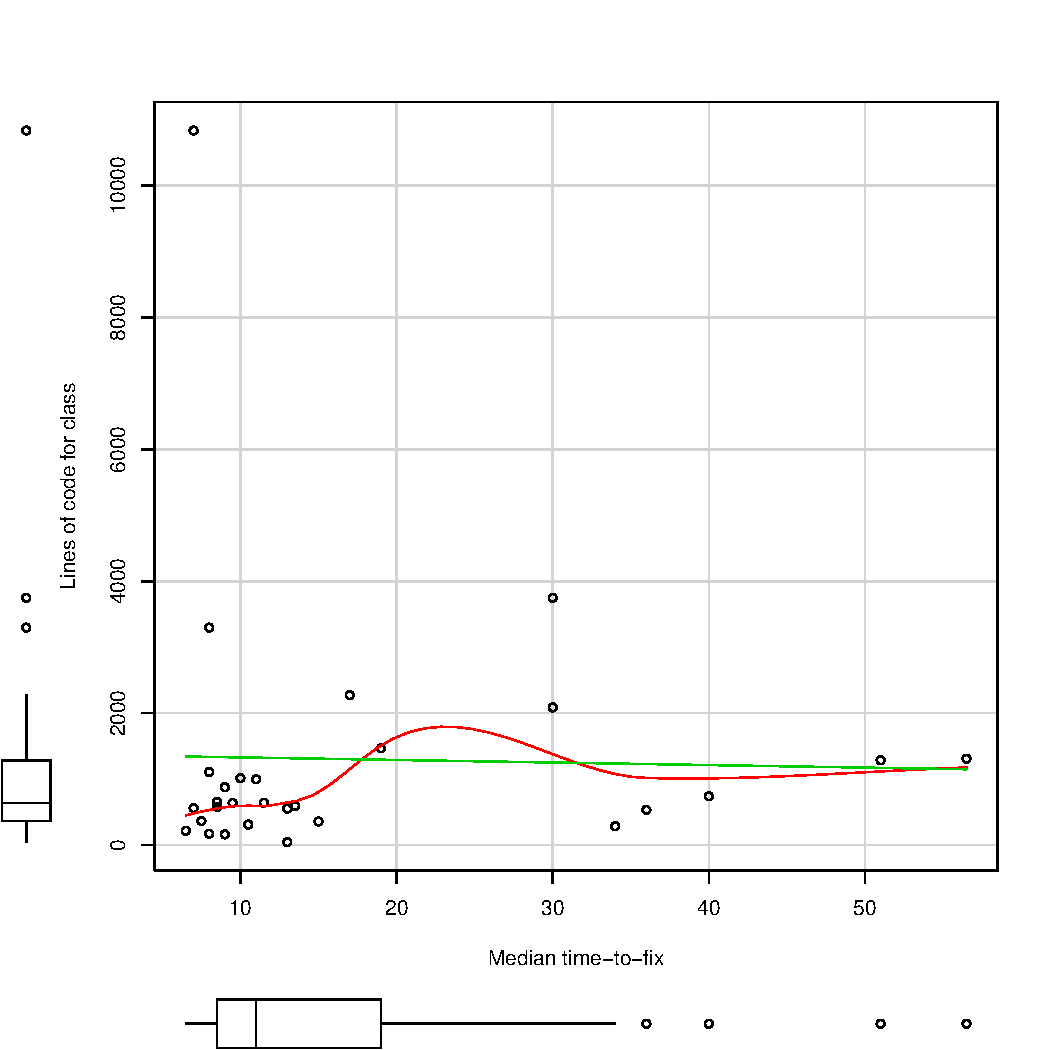
\includegraphics[width=1\textwidth]{img/ttf-classes-loc.pdf}
	\caption{Scatter plot of time-to-fix vs lines of code. On the x-axis, the median time-to-fix of all corresponding issues for a class is shown, where on the y-axis, the lines of code of the class are shown. The green solid line depicts a linear regression line, where the red solid line is a non-parametric Loess regression line ($f = 0.7$).}
	\label{fig:ttf_loc_scatter}
\end{figure}

% subsection results (end)

\subsection{Analysis} % (fold)
As can be seen in Figure~\ref{fig:ttf_loc_scatter}, no evident visual signs of correlation can be noticed between median time-to-fix and the corresponding class size. In order to statistically verify if a correlation is present, the Kendall tau-b rank correlation coefficient ($\tau_B$) is calculated. When the Kendall tau-b test (see Section~\ref{sub:kendall_tau_b_rank_correlation_coefficient}) is applied to the data set, the following $\tau_B$ value is found:

\begin{equation}
	\tau_B = 0.129
\end{equation}

The null hypothesis for the Kendall tau-b test states `there is no relationship between the two variables'. Since $\tau_B = 0.129$, a weak correlation can be expected to exists between the two variables. However, for this $\tau_B$, a $p$-value of 0.338 is found, meaning the null hypothesis that that the variables are statistically independent cannot be rejected. This large $p$-value is probably caused by the low number of data points and several outliers in the dataset.

% subsection analysis (end)

\subsection{Conclusions} % (fold)
The data set only has 29 data points due to the fact that not much bug reports have 10 or more matching classes. This is a limitation for the correlation analysis. As can be seen in the scatter plot in Figure~\ref{fig:ttf_loc_scatter}, no apparent correlation is shown. The Kendall tau-b test does not give a statistical significant result, meaning the null hypothesis that that the variables are statistically independent cannot be rejected. In conclusion, it is not possible to accept or reject hypothesis H2.3: 

\vspace{\baselineskip}
\hypbc{}

% subsection conclusions (end)

% section correlation_analysis_between_loc_and_ttf (end)

\section{Summary of results} % (fold)
\label{sec:ttf_summary_of_results}
This chapter showed the results and analysis for research question R2, as described in Chapter~\ref{sec:analysis:time_to_fix}:

\vspace{\baselineskip}
\questionb{}
\vspace{\baselineskip}

\noindent
First, it was investigated whether the time-to-fix of a bug decreases if a stack trace is present. A comparison between bug reports with and without a stack trace shows no difference between the median time-to-fix values. However, the descriptive statistics are promising, showing that both mean and median time-to-fix values decrease significantly when a stack trace is present. We therefore partially accept hypothesis H2.1.

Next, it was investigated if the time-to-fix decreases when a stack trace is present in the first comment of a bug report (compared to a trace in other comments). When comparing the median time-to-fix values again, a significant result is found. Hypothesis H2.2 therefore is accepted.

Finally, a possible relationship between class size and time-to-fix is investigated. Due to the limited amount of data available, it is not possible to state anything regarding hypothesis H2.3.
% section summary_of_results (end)

% chapter results_time_to_fix (end)

% part results (end)

\part{Conclusions} % (fold)
\label{prt:conclusions}
%!TEX root = thesis.tex

\chapter{Discussion and Implication of the Results} % (fold)
\label{cha:discussion_implication_of_the_results}
This chapter discusses the implications of the results found in the previous chapters in more detail. Also, potential threats to the validity of the results found during the experiments are discussed.

\section{Implication of the results} % (fold)
\label{sec:implication_of_the_results}
A total of two research questions are investigated in the previous chapters. In this section, the outcome of their hypotheses are discussed, including their implications for developers, reporters and bug triagers.

\subsection{Priority and severity} % (fold)
In Chapter~\ref{cha:results_priority_and_severity}, the hypotheses associated with research question R1 are evaluated:

\vspace{\baselineskip}
\questiona{}
\vspace{\baselineskip}

The first two hypotheses assess whether the presence of a stack traces results in a higher priority and severity. For \texttt{jdt.debug}, the statistical test does not show an association between priority and the presence of a stack traces. However, the relative number of high and low priority issues does change. For \texttt{jdt.core}, both the statistical test as well as the descriptive statistics show an association. For severity, for both datasets the statistical tests and descriptive statistics show an association with the presence of a stack trace. These results look promising. When a stack trace is present, both priority and severity show a particular shift, where the number of high priority and severity bugs increase, and the number of low priority and severity bugs decrease.

In \cite{Bettenburg2007} and \cite{Zimmermann2010}, it is shown that the presence of a stack trace is a sign of quality of a bug report. High quality bug reports are likely to get more attention from developers and triagers, which might also be why they get assigned a more representative priority and severity, instead of the default value.

Severity should be an absolute classification of a bug, i.e., in an ideal situation, the triager, developer, and reporter should all agree on this. However, in practice, reporters probably have less knowledge of the software than triagers and developers. In the end, the triager is the designated person to determine the severity of the bug. Schr\"{o}ter \emph{et al.} \cite{Schroter2010} showed that in up to 60\% of fixed bug reports, the bug is actually fixed in one of the methods mentioned in a stack trace. Stack traces therefore are valuable pointers to points of interest in the source code. This means that when a stack trace is present in the bug report, a triager might be able to perform a better assessment of the severity of a bug by inspecting the source code. This way, it might also be possible to assess a better priority for the bug report, since the possible costs for a fix might be easier to determine (by inspecting source code and related bugs).

When priority and severity are related to package size (higher package size results in a higher priority or severity), very little data is available. This is due to the fact that both the number of priorities and severities, as well as the number of packages is low. Combined with a high percentage of bug reports being assigned default priority and severity, the number of data points available for analysis is very low. This is consistent with the research performed in \cite{Lamkanfi2010}. Only in the case of \texttt{jdt.core} and severity, some investigations could be performed. However, these did not show any significant result that points to a possible relation of severity and package size. It should be considered to perform this investigation with data that is more suitable (i.e., has more non-default severity and non-default priority bug reports).

The final two hypotheses investigate a possible relation between priority and severity, and class size. For this, when class size increases, the priority and severity are expected to increase as well. Although the number of classes is much higher than the number of packages, again, there is a lack of data. This is once again due to the fact that a high number of bug reports is being assigned the default priority and severity. For the test with severity and class size for \texttt{jdt.debug}, no possible relation is found. When \texttt{jdt.core} and severity are investigated, no evidence of a shift in severity was found. Again, it should be considered to perform this investigation with data that is more suitable.

For now, using the data for this specific research, no evidence was found for a relation between priority and severity, and package and class size.

Overall, the main problem for these investigations is lack of data. The Eclipse projects under investigation seem to pay little attention to assigning a representative priority and severity, since for virtually all bug reports, the priority and severity are assigned the default values. This is not considered as a threat to validity, but most certain is disappointing for this research, since a careful investigation of some of the hypotheses is made impossible. However, this could be tackled by importing data of more projects or using different open source projects that do use priority and severity in a consistent way.

Concluding, evidence is found that both priority and severity tend to show a particular shift when a stack trace is present. It is shown that, in presence of a stack trace, more high priority and high severity reports are present, and less low priority and severity bugs. Severity seems a good candidate for a prediction model, since it is an absolute classification of a bug report. Input for such a model can, for example, be bug reports that are related to the report under investigation by stack trace frames. Priority on the other hand might be harder to predict, since assigning a priority to a bug report is mainly considered a cost-benefit decision. But again, related bugs might be a suitable source for a prediction model. 

For developers, no immediate use is found for the results, except for using stack traces in finding relevant pointers to the source code and to related bugs. For bug reports, adding a stack trace could be a good incentive to increase the priority and severity of a bug. Bugs reports that are considered high quality reports will get more attention from triagers, which might result in a more representative priority and severity. 

\subsection{Time-to-fix} % (fold)
The hypotheses associated with research question R2 are evaluated in Chapter~\ref{cha:results_time_to_fix}:

\vspace{\baselineskip}
\questionb{}
\vspace{\baselineskip}

First, it is investigated whether the time-to-fix of an issue decreases when a stack trace is present. Since only the complete bug repository for \texttt{jdt.debug} is imported, only this data set is taken in consideration. Although for \texttt{jdt.core}, still only a limited amount of imported bug reports contains an actual stack trace, we believe there might still be a bias. 

The descriptive statistics for \texttt{jdt.debug} are promising, but the statistical test and further investigation of the data show no evidence for a decrease in time-to-fix. Our statistical results are not consistent with the work of Schr\"{o}ter \emph{et al.} \cite{Schroter2010}, who found strong evidence that bug reports that include one or more stack traces do indeed have a shorter lifetime. They also found that the lifetime of a bug decreases even further when the bug is fixed in a method mentioned in one of the stack frames. This corresponds with our descriptive statistics, which show that both the mean and median time-to-fix decreases significantly when a stack trace is present. In order to reach a conclusive result on this, more data should be investigated. Concluding, we partially accept the hypothesis that the time-to-fix of an issue decreases when a stack trace is present.

Next, an investigation is performed to see if the time-to-fix decreases when the stack traces are in the \emph{first} comment of the bug report, compared to a bug report with stack traces in non-first comments. For \texttt{jdt.debug}, no statistical significant result is found. However, both the mean and median time-to-fix values increase quite a lot when a stack traces are present in the non-first comments. For \texttt{jdt.core} and the overall data set, a highly significant change is found. Due to the small sample size for \texttt{jdt.debug}, outliers probably have quite some influence on the statistics. This leads to the conclusion that the time-to-fix of a bug decreases significantly when the stack trace is present in the first comment of the bug report. This is consistent with the results of Schr\"{o}ter \emph{et al.} \cite{Schroter2010}. As mentioned before, they found strong evidence that bug reports that include one or more stack traces do indeed have a shorter lifetime. They also found that the lifetime of a bug decreases even further when the bug is fixed in a method mentioned in one of the stack frames. Regarding stack trace position in the bug report, they found that 70\% of the bugs were fixed in a stack frame from the \emph{first} stack trace in the bug report.

Finally, a correlation analysis between class size and time-to-fix is performed. Again, the size of the data set is very small. Both visually and statistically, no correlation could be found. No previous work for this investigation was found. This investigation should again be performed with more data to get conclusive results.

Again, the lack of data is an issue in the investigations. On the total number of issues imported, only a small percentage contains a stack trace. Overall this percentage is only 6.5\%, which is even lower than the 11\% found by Anvik \cite{Anvik2006}. An even smaller part can be matched to the source code and source code version history models. This funnel effect makes that in practice the number of data points in the actual data sets eligible for investigation, is very limited, especially when a minimum of matching classes is required for an investigation. This was not something that was expected on beforehand, but makes the third investigation impossible to be taken into consideration when answering research question R2.

Concluding, presence of a stack trace and the position of this stack trace in the bug report both seem interesting features to use in a prediction model for fix time. Also, other properties can be taken into consideration, as described in \cite{Kim2006,Weiss2007,Panjer2007,Giger2010}, such as number of comments in related bug reports or the severity of related bug reports \cite{Weiss2007}. For reporters, it might be a great incentive to add stack traces to their bug reports, if they are aware that this might speed up fixing their bug. Triagers can use stack traces to, preferably automatically, find previous related bugs in order to assess the projected time-to-fix more accurately. Also, prediction algorithms can automate this task even further. For developers, stack traces are again considered as a helpful instrument in fixing a bug. They provide valuable pointers to related source code, that might speed up fixing a bug. Also, related bugs might give great insights in related fixes that are already applied to the software. For example, this can help in identifying regression bugs.

% section implication_of_the_results (end)

\section{Threats to validity} % (fold)
\label{sec:threats_to_validity}
The results of the research performed in this thesis are subject to several threats to validity. The following threats to validity will be discussed:

\begin{itemize}
	\item Construct validity: Are the experiments measuring what they claim to measure?
	\item Internal validity: Are conclusions about possible causal relationships valid?
	\item External validity: Can the findings of the study be generalised?
	\item Statistical validity: Are the statistical tests accurate and correctly interpreted?
\end{itemize}

\subsection{Construct validity} % (fold)
\label{sub:construct_validity}
In this research, several possible relations are investigated:

\begin{itemize*}
	\item Priority versus presence of a stack trace;
	\item Priority versus package size;
	\item Priority versus class size;
	\item Severity versus presence of a stack trace;
	\item Severity versus package size;
	\item Severity versus class size;
	\item Time-to-fix versus presence of a stack trace;
	\item Time-to-fix versus position of the stack trace in comments;
	\item Time-to-fix versus class size.
\end{itemize*}

The definitions for priority, severity, time-to-fix, presence of a stack trace, position of a stack trace, package size and class size are clearly stated.

The actual research framework used should match the conceptual model. For this, suitable meta-models should be selected, after which data sets can be imported and extracted. 

\subsubsection{Model selection} % (fold)
The Evolizer tool \cite{Gall2009,Ghezzi2008,Ghezzi2010}, that has been used in many existing studies \cite{Fischer,Fischer2003,D'Ambros2006,D'Ambros2007,Fischer2004,Pinzger2005}\footnote{also including work of the authors where the RHDB is used, which in turn is included in Evolizer}, includes a model for source code, source code history and bug reports. A potential risk concerns the quality of these models. Thorough investigations are performed to make sure all these models represent the real-world scenarios in a correct way. 

A model for stack traces was not included in the Evolizer tool. Support for stack traces is added. With this model and the changes applied, the actual research framework is able to represent the conceptual model.

\subsubsection{Importing data} % (fold)
In order to provide the model with actual data, all data from the source code and issue repositories is imported. A possible risk concerns the integrity of the data. Several manual checks are performed to make sure the imported data equals the actual data in the repositories.

During these checks, several bugs in the importer have been found. They have all been mitigated in order to ensure a correct import. 

\subsubsection{Availability} % (fold)
After importing data, the model should be a complete representation of the actual source repositories. Due to the amount of time importing a full version history repository takes, for \texttt{jdt.core} not all issues have been imported. This is a threat to the time-to-fix versus presence of a stack trace investigation. 

To mitigate this risk, \texttt{jdt.core} data is excluded from this particular investigation.

\subsubsection{Model extraction} % (fold)
Based on the data imported, several models are extracted. The readily available extractions in Evolizer have been used in several publications \cite{Gall2009,Ghezzi2008,Ghezzi2010}. Therefore, there is no particular reason to doubt the correct functioning of the extraction. To be sure, a manual quality check has been performed.

The current issue model is extended to have support for stack traces. Again, this is thoroughly tested to ensure correct behavior. This also applies to the matching algorithm for stack traces to the FAMIX and source code model.

For this research, all issues are matched to only one FAMIX model. It would have been better to use several FAMIX models, representing the changes in source code over time. For example, one FAMIX model per tagged release could be used. However, since this research only uses package and class level granularities, this functionality was not implemented into Evolizer. Preliminary investigation of the used data sources showed that package and class names are relatively stable.

\subsubsection{Metric calculation} % (fold)
All metrics used should represent the actual real-world values and should be calculated correctly. In order to match the conceptual model, Evolizer is extended with two more metrics of package size. The time-to-fix metric has been altered to a more strict definition.

In order to avoid any thread to validity, all metrics are strictly defined. Also, the actual calculations are tested and also checked manually.

One threat to validity is the source code used to calculate time-to-fix for a class. Only the latest checked in revision is used for this, since it is quite hard to reliable relate a specific bug report to a specific revision of the source code file.
% subsection construct_validity (end)

\subsection{Internal validity} % (fold)
Internal validity is about cause and effect. It tells something about the degree to which conclusions about cause and effect can be made, based on the research design. 

In this research, only relations between relatively simple metrics are considered. It is of the utmost importance that these metrics do not change over time, for example by change of behavior in the usage of the source repositories. Several descriptive statistics about the data sets show no evidence for this.

No further threats to internal validity are found. All investigations performed have a solid hypothesis. Also, no external threats are found during the research that could have had influence on the measurements.

Finally, all data used is documented and imported to a fixed data set. This means the actual research performed can be reproduced.
% subsection internal_validity (end)

\subsection{External validity} % (fold)
The research framework and methodology used can be easily used for other software projects and their associated repositories. However, this particular research has only been applied to two specific projects from the Eclipse open source project. Both the fact that only open source projects are considered, as well as the limited amount of projects under tests, are a threat to validity. 

The goal of this research was to investigate the potential of stack traces in the assessment of bug report properties, and to develop a useful research framework for this. For future work, it is recommended to repeat this research on a wider range of projects, both open source and commercial.
% subsection external_validity (end)

\subsection{Statistical validity} % (fold)
\label{sub:statistical_validity}
To make sure the statistical tests used in this thesis are applied correctly, much effort is put into research of available statistical methods. For each situation, the assumptions a specific test makes are taken into consideration, such a normality of data and size of the data sets. Also, considerable effort is put into correct interpretation of the outcome of the tests.

To achieve a valid result, the number of data points in each data set should be considerable. This is not the case for all data sets. This was not something that was expected on beforehand.
% subsection statistical_validity (end)

% section threats_to_validity (end)
% chapter discussion_implication_of_the_results (end)
%!TEX root = thesis.tex

\chapter{Conclusions and Future Work} % (fold)
\label{cha:conclusions_and_future_work}
In this chapter, the conclusions for this thesis will be summarised. Also, some pointers for future work are given.

\section{Conclusions} % (fold)
In software engineering, resources such as time, money and developers, are limited. Often when bugs are found in the software developed, bug triaging is used to prioritise bug reports and allocate resources to it. In large (open source) software projects, the number of bug reports can be considerable. When each of these bugs should be analysed by a bug triager, this will require a vast amount of time and effort. In order to assist the bug triager in the assessment of a bug, a large amount of data is already available. The goal of this research is to investigate the usefulness of stack traces in bug reports for the assessment of bug report properties, such as severity, priority and time-to-fix.

In order to investigate the research questions and hypotheses, a research framework is developed. This framework consists of four major parts: source code extraction, issue report extraction and stack trace matching are used to create a consistent data set. After this, data analysis is applied to the data set to investigate our hypotheses. During this analysis, appropriate data sets are constructed for each hypothesis, which are in turn investigated using visualisations and descriptive statistics, as well as statistical research.

Overall, we can conclude that stack traces can be used to link software artifacts. Also, stack traces can be a valuable input for prediction models, for example using metrics of related bugs and source files. Finally, lack of data makes that not all hypotheses in this thesis are conclusive. 

The results of all hypotheses are summarised below.

\subsection{Research question 1} % (fold)

\questiona{}

\vspace{\baselineskip}
\hypaa{}
\vspace{\baselineskip}

\noindent
The statistical analysis is not fully conclusive, but the particular shift in priority when a stack trace is present gives enough evidence to at least partially accept this hypothesis.

\vspace{\baselineskip}
\hypab{}
\vspace{\baselineskip}

\noindent
Both the statistical analysis as well as the particular shift in severity when a stack trace is present gives enough evidence to accept this hypothesis.

\vspace{\baselineskip}
\hypac{}
\vspace{\baselineskip}

\noindent
Due to a lack of data, we cannot conclude anything on this hypothesis.

\vspace{\baselineskip}
\hypad{}
\vspace{\baselineskip}

\noindent
Some investigations are performed, but no evidence is found for an association between package size and severity. This hypotheses is rejected.

\vspace{\baselineskip}
\hypae{}
\vspace{\baselineskip}

\noindent
Due to a lack of data, we cannot conclude anything on this hypothesis.

\vspace{\baselineskip}
\hypaf{}
\vspace{\baselineskip}

\noindent
Some investigations are performed, but no evidence is found for an association between class size and severity. This hypotheses is  rejected.

Evidence is found that both priority and severity tend to show a particular shift when a stack trace is present. It is shown that, in presence of a stack trace, more high priority and severity reports are present, and less low priority and severity bugs. Regarding package and class size, insufficient data is available to conclude anything on this. However, some evidence is found for the lack of an association between package or class size, and priority and severity. 

Overall, the main problem for these investigations is lack of data. The Eclipse projects under investigation seem to pay little attention to assigning a representative priority and severity, since for virtually all bug reports, the priority and severity get assigned the default values. However, this could be tackled by importing data of more projects or using different open source projects that do use priority and severity in a consistent way.

Concluding, the presence of a stack trace tends to result in more high priority and severity bugs, and less low priority and severity bugs. Severity seems a good candidate for a prediction model, since it is an absolute classification of a bug report. Priority on the other hand might be harder to predict, since assigning a priority to a bug report is mainly considered a cost-benefit decision. Still, related bugs might be a suitable source for a prediction model. Beyond that, in this thesis, no other metrics are found to be useful to predict the priority and severity of a bug report.

\subsection{Research question 2} % (fold)

\questionb{}

\vspace{\baselineskip}
\hypba{}
\vspace{\baselineskip}

\noindent
Although the descriptive statistics looked promising, no statistical evidence is found for a decrease in time-to-fix when a stack trace is present. However, the work of Schr\"{o}ter \emph{et al.} \cite{Schroter2010} supports our descriptive statistics, which show that both the mean and median time-to-fix decreases significantly when a stack trace is present. In order to reach a conclusive result on this, more data should be investigated. This hypothesis is partially accepted.

\vspace{\baselineskip}
\hypbb{}
\vspace{\baselineskip}

\noindent
Strong evidence is found for a decrease in time-to-fix when one or more stack traces are present in the first comment of a bug report, compared to the presence one or more stack traces in the remaining comments. This is consistent with the work of Schr\"{o}ter \emph{et al.} \cite{Schroter2010}. This hypothesis is accepted.

\vspace{\baselineskip}
\hypbc{}
\vspace{\baselineskip}

\noindent
Little data is available, and this data does not show a correlation between class size and median time-to-fix. Due the limited amount of data, is is not possible to accept or reject this hypothesis.

Concluding, presence of a stack trace and the position of this stack trace in the bug report both seem interesting features to use in a prediction model for fix time. Time-to-fix of a bug is positively affected by the presence of a stack trace, especially when this stack trace is in the first comment of the bug report. Based on the research performed in this thesis, we found evidence that stack traces might be useful in predicting the the time-to-fix.

% section conclusions (end)

\section{Future work} % (fold)
\label{sec:future_work}
This work is an exploratory search for interesting relations between software repository metrics and bug report properties. Despite initial optimism of the usage of stack traces, a thorough analysis of the data shows less promising results. Also, both the positive outcomes as well as the negative outcomes are subject to several threats to validity. 

One improvement to this research is to apply it to more software projects, instead of just two projects from Eclipse. Both open source and closed source projects should be considered. With the selection of these projects, one should take into account the usage of priority and severity (are they used properly?). Also, sufficient data should be available. The funnel effect makes this research is almost only applicable to large data sets, i.e., projects with a long history.

Next to this, the history of the source code should be taken into account. Not one FAMIX model and one source code model should be used, but several, for example one for each tagged release of the software. This way, older bugs have a more appropriate source code model to apply measurements to.

For time-to-fix, we can make a distinction between stack traces that are added to the bug report before triaging (i.e., changing status to `confirmed') and stack traces that are added later on. Also, the number of comments before triaging might be interesting.

When investigating a possible relation between class size and time-to-fix, one might also take into account the position of the stack frame in the stack trace. This position should be calculated by discarding all external classes (that are used in libraries for example), so we can focus on classes that have an actual size in the source repository.

Next to priority, severity and time-to-fix, other bug report properties could be researched. For example, the most suiting developer to fix a specific bug could be detected using previous commits made to specific source files that are mentioned in the stack traces in a bug report. This study was not performed in this thesis, due to the fact that the number of core developers was very limited. Therefore, they were accountable for most commits. This could also be explained by the method of work of the Eclipse developer, where a small number of developers is responsible for committing actual changes by other developers.

It might be also interesting to apply triaging tools to online software-as-a-service solutions, such as Github\footnote{\url{https://github.com/}}, Google Code\footnote{\url{http://code.google.com/}} or Codeplex\footnote{\url{http://www.codeplex.com/}}. These online repositories host a vast amount of both closed and open source projects. Also, tools such as wikis and issue trackers, are often already integrated. But far and foremost, most of these repositories contain a lot of `social coding' projects, where a lot of developers assist in the development of software.

Finally, the FAMIX source code model can be used to determine a specific subsystem of the software where a bug occurred. Based on the issue history, a suitable developer might be found with adequate knowledge of this subsystem. By choosing the correct developer, `bug ping pong' can be prevented.

% section future_work (end)

% chapter conclusions_and_future_work (end) 
% part conclusions (end)

\bibliographystyle{plain}
\bibliography{thesis}

\appendix
\def\chaptername{Appendix}
%!TEX root = thesis.tex

\chapter{Bugzilla importer XML parser issues} % (fold)
\label{cha:bugzilla_importer_xml_parser_issues}
When parsing Bugzilla data using the XML parser, several issues were found. A SAX parser has an event-based API, meaning the parser calls certain user specified callback methods when an event occurs. These events include the start and end of an XML element, and reading character in between these elements. The SAX parser in Evolizer was fundamentally broken. According to the specification\footnote{\url{http://www.saxproject.org/apidoc/org/xml/sax/ContentHandler.html}}, the SAX2 parser has several callback methods, of which three were implemented in Evolizer: \texttt{startElement}, \texttt{endElement} and \texttt{characters}. Let's say the following XML fragment is read by the parser:

\begin{quote}
\texttt{<commentid>64872</commentid>}
\end{quote}

\noindent
When the start element is read, the \texttt{startElement} callback method is called. Similar, at the end of this line, the \texttt{endElement} callback method is called. When reading the data in between the XML tags, the \texttt{characters} method is called. A state machine is used to keep track of the elements that are read and makes that the data is converted into model classes. In this case, the ID of a \texttt{Comment} object would be set after the XML fragment was read. 

Typically, state changes occur in the \texttt{startElement} and \texttt{endElement} methods. However, in Evolizer, the \texttt{characters} method was used for changing state. When reading characters in between a start and end element in XML, the \texttt{characters} callback method can be invoked \emph{multiple times} in order to read all data. In Evolizer, it was assumed the \texttt{characters} callback would only be called once (or twice, according to source code comments). This design choice resulted in unpredictable state changes and reading incomplete data\footnote{It probably would have been a better design choice to use a XML parser that is able to \emph{unmarshall} XML directly to the POJOs representing the meta-model. Although this approach has an impact on speed, this will not be noticed, since a pause of around a second is already present between consecutive bug imports.}.

The issues mentioned above were mitigated by correctly implementing the state machine. This resulted in correct state change behavior and reading of all data in between XML tags.
% chapter bugzilla_importer_xml_parser_issues (end)
%!TEX root = thesis.tex

\chapter{Normality test results} % (fold)
\label{cha:normality_tests}
The D'Agostino test is a suitable test for normality. This test calculates the skewness and kurtosis of the data and compares this data with the expected values from a Gaussian distribution. With this test, the null hypothesis states the data is sampled from a Gaussian distribution. This appendix contains all normality tests performed in this thesis.

\section{Priority and severity} % (fold)
\label{sec:priority_and_severity}

\subsection{Package size} % (fold)
\label{sub:norm:package_size}
The distributions of the data sets is depicted in Figure~\ref{fig:packages-density-sevcore}. Nothing can be said about the distribution of the data, except that is roughly similar shaped.  The results for the D'Agostino tests of all twelve data sets are shown in Table~\ref{tab:package-sev-core-agostino}. As can be seen, none of the $p$-values is higher than a significance level of $\alpha = 0.001$, meaning we reject the null hypothesis that the data sets follows a Gaussian distribution. For severity `normal' for the metrics NOC and SUMLOC, the D'Agostino test does not give a result. However, based on the density graph, it can be assumed the data is also not normal distributed.

\begin{figure}
        \begin{subfigure}[b]{0.5\textwidth}
                \centering
                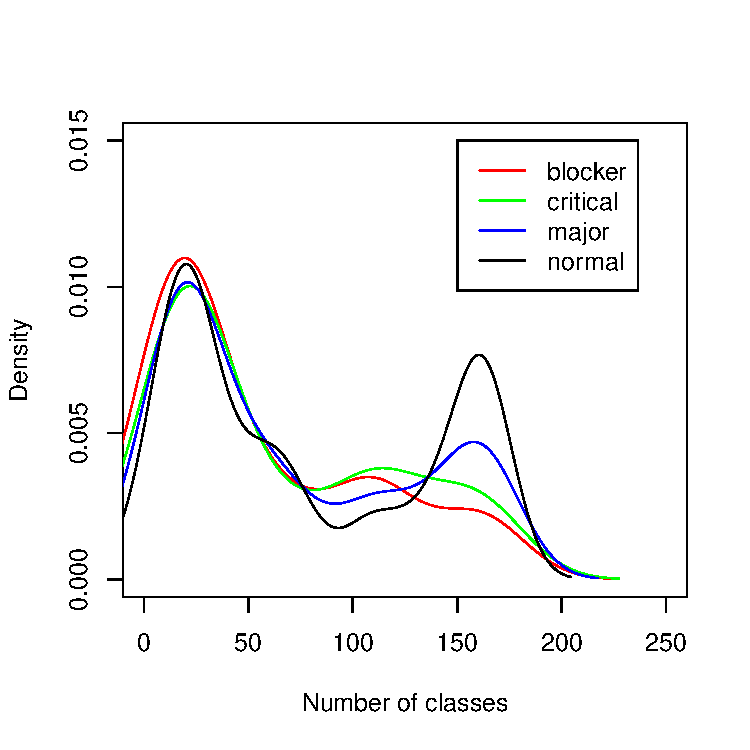
\includegraphics[width=\textwidth]{img/sev-core-noc-density.pdf}
                \caption{NOC}
                \label{fig:density-sevcore-noc}
        \end{subfigure}%
        ~ %add desired spacing between images, e. g. ~, \quad, \qquad etc. 
          %(or a blank line to force the subfigure onto a new line)
        \begin{subfigure}[b]{0.5\textwidth}
                \centering
                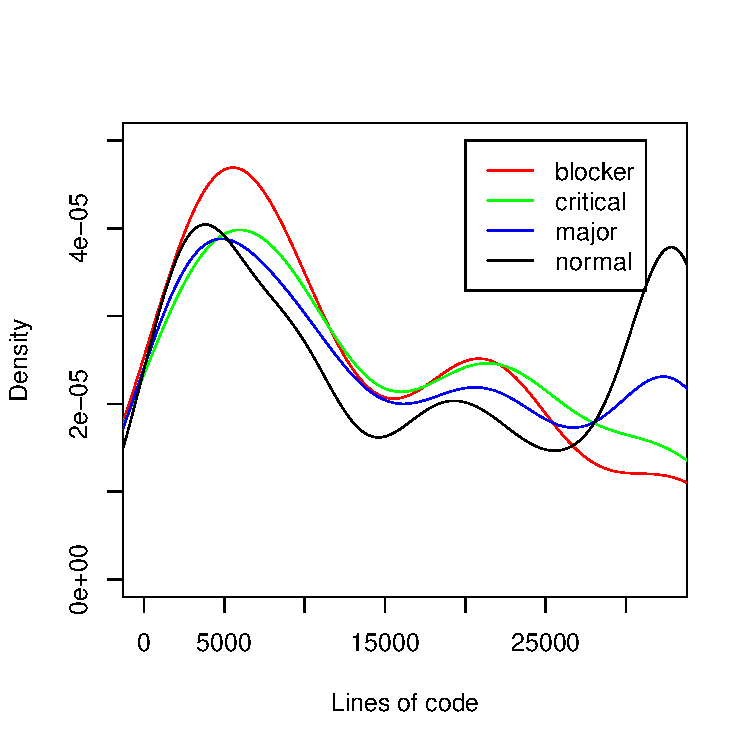
\includegraphics[width=\textwidth]{img/sev-core-sumloc-density.pdf}
                \caption{SUMLOC}
                \label{fig:density-sevcore-sumloc}
        \end{subfigure}

        \begin{subfigure}[b]{0.5\textwidth}
                \centering
                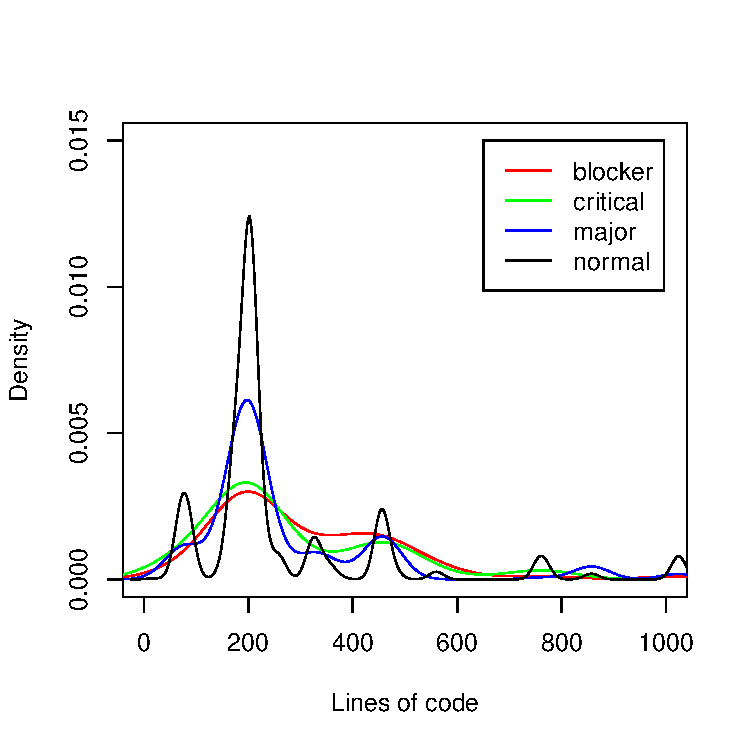
\includegraphics[width=\textwidth]{img/sev-core-avgloc-density.pdf}
                \caption{AVGLOC}
                \label{fig:density-sevcore-avgloc}
        \end{subfigure}
        \caption{Density graph for the distribution of data under investigation (jdt.core).}
        \label{fig:packages-density-sevcore}
\end{figure}

\begin{table}[!ht]\footnotesize
	\centering
	\begin{tabular}{lrl}
		\toprule
		Data set & p-value & \\
		\midrule
		NOC \\ 
		\midrule
		Blocker & $0.013$ & * \\
		Critical & $0.002$ & ** \\
		Major & $< 0.001$ & *** \\
		Normal & --\\\\
		\midrule
		SUMLOC \\
		\midrule
		Blocker & $0.026$ & * \\
		Critical & $0.002$ & ** \\
		Major & $< 0.001$ & *** \\
		Normal & -- \\\\
		\midrule
		AVGLOC \\
		\midrule
		Blocker & $< 0.001$ & *** \\
		Critical & $< 0.001$ & *** \\
		Major & $< 0.001$ & *** \\
		Normal & $< 0.001$ & *** \\
		\bottomrule
	\end{tabular} 
	\caption{D'Agostino normality test results for data under investigation. $p$-values could not be calculated for severity `normal' for metrics NOC and SUMLOC.}
	\label{tab:package-sev-core-agostino}
\end{table}

% subsection package_size (end)

\subsection{Class size} % (fold)
\label{sub:norm:class_size}
The distributions of the data sets is depicted in Figure~\ref{fig:class-sev-core-density}. Although it might look a bit like a normal distribution, the graph is zoomed in heavily. Nothing can be said about the distribution of the data, except that is roughly similar shaped. The results for all six data sets are shown in Table~\ref{tab:class-sev-core-agostino}. As can be seen, none of the p-values is higher than a significance level of $\alpha = 0.001$, meaning we reject the null hypothesis that the data sets follows a Gaussian distribution.

\begin{table}[!ht]\footnotesize
	\centering
	\begin{tabular}{lrl}
		\toprule
		Data set & p-value & \\
		\midrule
		Blocker & $< 0.001$ & *** \\
		Critical & $< 0.001$ & *** \\
		Major & $< 0.001$ & *** \\
		Normal & $< 0.001$ & *** \\
		Minor & $< 0.001$ & *** \\
		\bottomrule
	\end{tabular} 
	\caption{D'Agostino normality test results for data under investigation.}
	\label{tab:class-sev-core-agostino}
\end{table}

\begin{figure}[!ht]
	\centering
		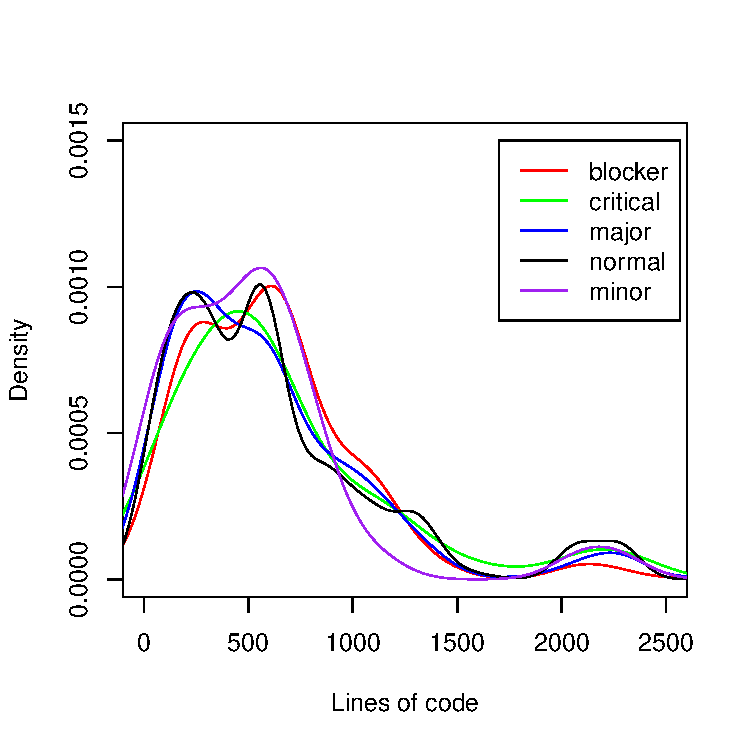
\includegraphics[width=0.7\textwidth]{img/sev-core-density.pdf}
	\caption{Density graph for the distribution of data under investigation (jdt.core).}
	\label{fig:class-sev-core-density}
\end{figure}

% subsection class_size (end)
% section priority_and_severity (end)

\section{Time-to-fix} % (fold)

\subsection{Presence of stack trace} % (fold)
\label{sub:norm:presence_of_stack_trace}
\begin{figure}[!ht]
	\centering
		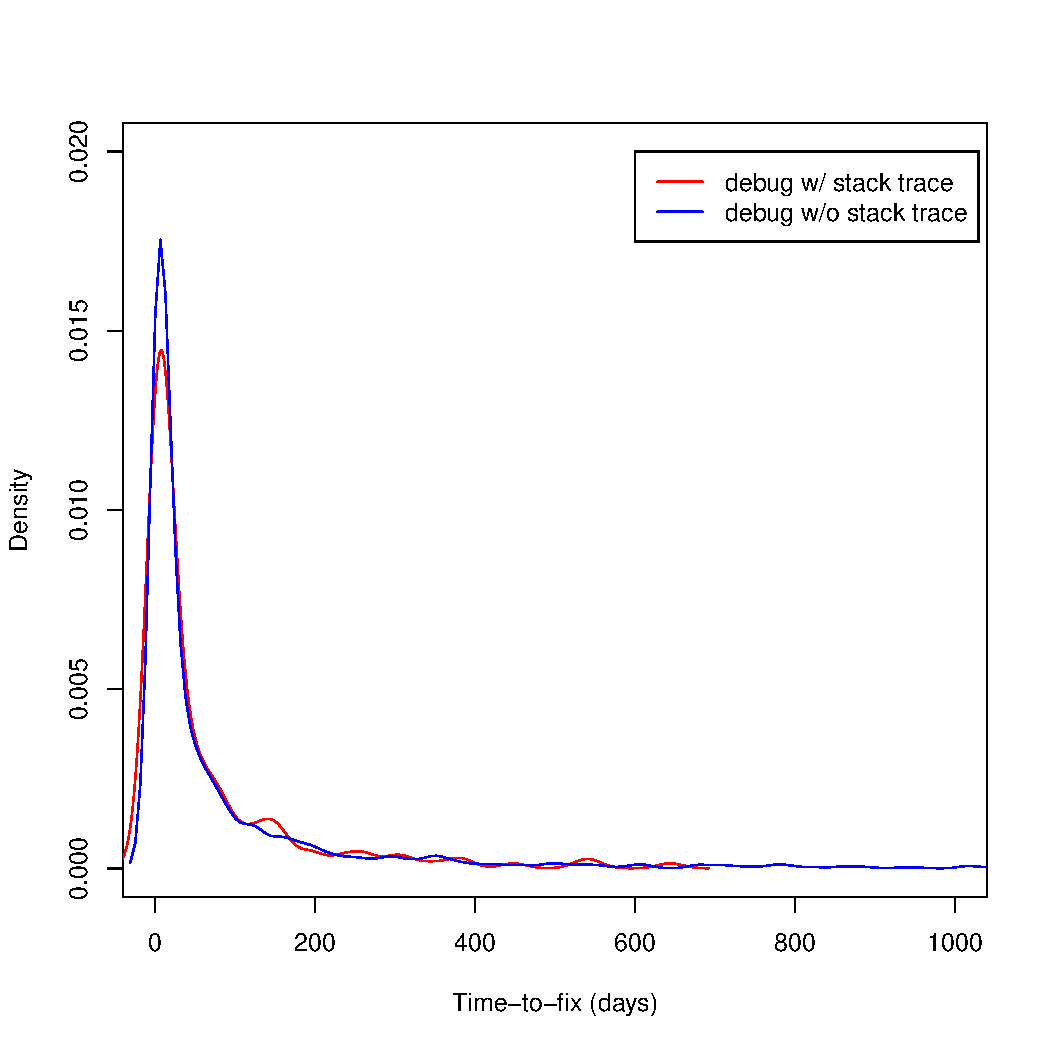
\includegraphics[width=1\textwidth]{img/ttf_with_without_stacktrace_density.pdf}
	\caption{Density plot of the data sets}
	\label{fig:ttf_density_plot}
\end{figure}

In Table~\ref{tab:ttf_stats}, the mean values are much larger than the median values. This is a characteristic of a \emph{skewed} distribution, where the skew measures the symmetry of a distribution. The skewness of the data can also be seen in Figure~\ref{fig:ttf_density_plot}, which shows the density plots of the data sets. The graph shows a Gaussian shape bell, but also shows a large tail which contains the outliers in the data. Figure~\ref{fig:ttf_density_plot} also shows the data sets have a similar shaped distribution.

These observations are a sign the data is not normally distributed. The results for all six data sets are shown in Table~\ref{tab:dagistino}. As can be seen, none of the p-values is higher than a significance level of $\alpha = 0.001$, meaning we reject the null hypothesis that the data sets follows a Gaussian distribution. 

\begin{table}[!ht]\footnotesize
	\centering
	\begin{tabular}{lrl}
		\toprule
		data set & p-value & \\
		\midrule
		jdt.debug with stack trace & $< 0.001$ & *** \\
		jdt.debug without stack trace & $< 0.001$ & *** \\
		\bottomrule
	\end{tabular} 
	\caption{D'Agostino normality test results.}
	\label{tab:dagistino}
\end{table}
% subsection presence_of_stack_trace (end)

\subsection{Stack trace position} % (fold)
\label{sub:norm:stack_trace_position}
In Table~\ref{tab:ttf_pos_stats}, the mean values are much larger than the median values. This is, again, a characteristic of a \emph{skewed} distribution. The skewness of the data can also be seen in Figure~\ref{fig:ttf_pos_stats_density}, which shows the density plots of the data sets. The graph shows a Gaussian shape bell, but also shows a large tail which contains the outliers in the data. The density plot also shows the data for jdt.core with stack traces in non-first comments has less outliers, which is of course also reflected in the overall density plot. Overall, all density plots are highly skewed and have a long tail.

These observations are a sign the data is not normally distributed. The results for all six data sets are shown in Table~\ref{tab:pos_dagistino}. As can be seen, none of the p-values is higher than a significance level of $\alpha = 0.01$, meaning we reject the null hypothesis that the data sets follows a Gaussian distribution. 

\begin{figure}[!ht]
	\centering
		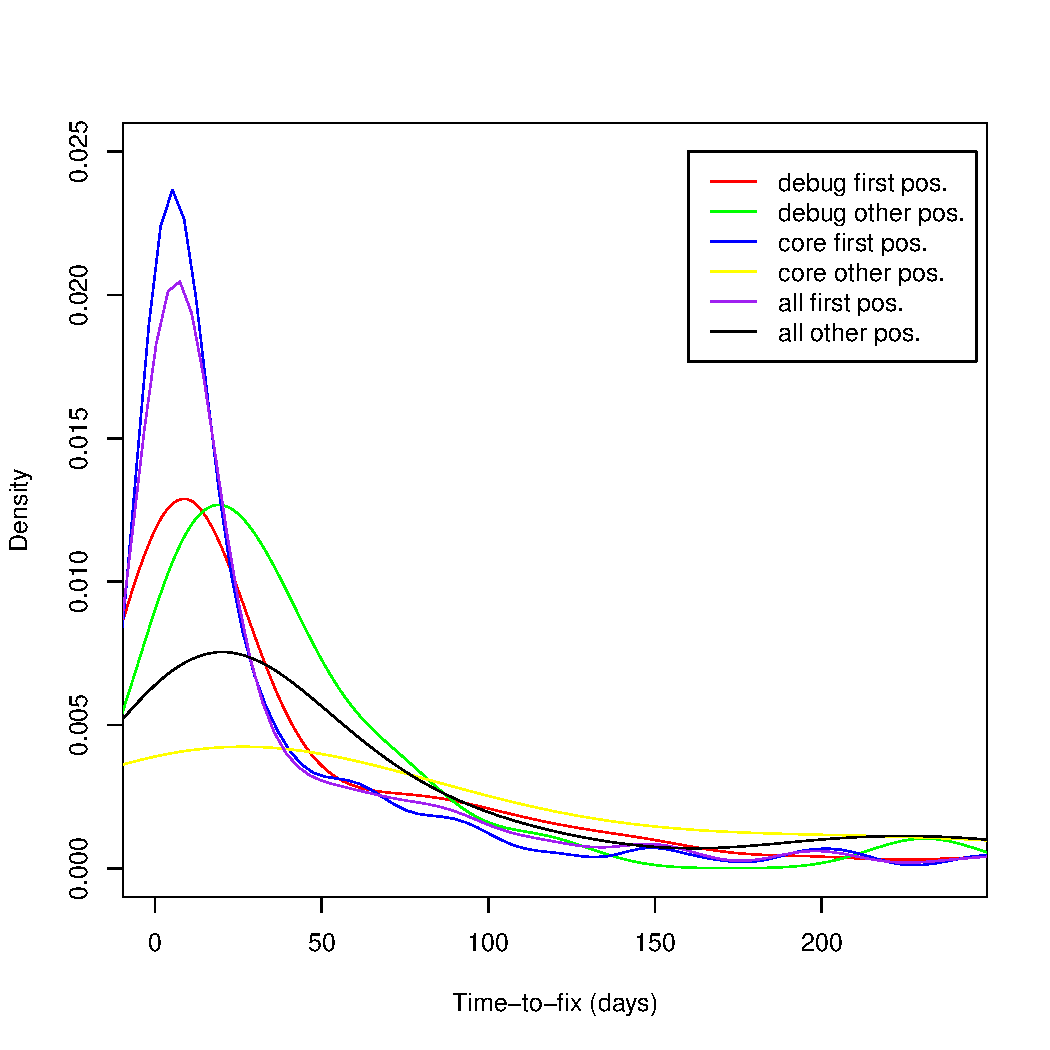
\includegraphics[width=1\textwidth]{img/ttf_stacktrace_pos_density.pdf}
	\caption{Density plot of the data sets (zoomed)}
	\label{fig:ttf_pos_stats_density}
\end{figure}

\begin{table}[!ht]\footnotesize
	\centering
	\begin{tabular}{lrl}
		\toprule
		data set & p-value & \\
		\midrule
		jdt.debug with stack traces in first comment & $< 0.001$ & *** \\
		jdt.debug with stack traces in non-first comments & $< 0.001$ & *** \\
		jdt.core with stack traces in first comment & $< 0.001$ & *** \\
		jdt.core with stack traces in non-first comments & $< 0.001$ & *** \\
		overall with stack traces in first comment & $< 0.001$ & *** \\
		overall with stack traces in non-first comments & $< 0.001$ & *** \\
		\bottomrule
	\end{tabular} 
	\caption{D'Agostino normality test results.}
	\label{tab:pos_dagistino}
\end{table}
% subsection stack_trace_position (end)

% section time_to_fix (end)

% chapter normality_tests (end)


\end{document}